%&preformat-disser
\RequirePackage[l2tabu,orthodox]{nag} % Раскомментировав, можно в логе получать рекомендации относительно правильного использования пакетов и предупреждения об устаревших и нерекомендуемых пакетах
% Формат А4, 14pt (ГОСТ Р 7.0.11-2011, 5.3.6)
\documentclass[a4paper,14pt,oneside,openany]{memoir}

%%%%%%%%%%%%%%%%%%%%%%%%%%%%%%%%%%%%%%%%%%%%%%%%%%%%%%%%%%%%%%%%%%%%%%%%%%%%%%%%
%%%% Файл упрощённых настроек шаблона, общих для диссертации и автореферата %%%%
%%%%%%%%%%%%%%%%%%%%%%%%%%%%%%%%%%%%%%%%%%%%%%%%%%%%%%%%%%%%%%%%%%%%%%%%%%%%%%%%

%%% Режим черновика %%%
\makeatletter
\@ifundefined{c@draft}{
  \newcounter{draft}
  \setcounter{draft}{0}  % 0 --- чистовик (максимальное соблюдение ГОСТ)
                         % 1 --- черновик (отклонения от ГОСТ, но быстрая
                         %       сборка итоговых PDF)
}{}
\makeatother

%%% Использование в pdflatex шрифтов не по-умолчанию %%%
\makeatletter
\@ifundefined{c@usealtfont}{
  \newcounter{usealtfont}
  \setcounter{usealtfont}{1}    % 0 --- шрифты на базе Computer Modern
                                % 1 --- использовать пакет pscyr, при его
                                %       наличии
                                % 2 --- использовать пакет XCharter, при наличии
                                %       подходящей версии
}{}
\makeatother

%%% Использование в xelatex и lualatex семейств шрифтов %%%
\makeatletter
\@ifundefined{c@fontfamily}{
  \newcounter{fontfamily}
  \setcounter{fontfamily}{1}  % 0 --- CMU семейство. Используется как fallback;
                              % 1 --- Шрифты от MS (Times New Roman и компания)
                              % 2 --- Семейство Liberation
}{}
\makeatother

%%% Библиография %%%
\makeatletter
\@ifundefined{c@bibliosel}{
  \newcounter{bibliosel}
  \setcounter{bibliosel}{1}   % 0 --- встроенная реализация с загрузкой файла
                              %       через движок bibtex8;
                              % 1 --- реализация пакетом biblatex через движок
                              %       biber
}{}
\makeatother

%%% Вывод типов ссылок в библиографии %%%
\makeatletter
\@ifundefined{c@mediadisplay}{
  \newcounter{mediadisplay}
  \setcounter{mediadisplay}{2}   % 0 --- не делать ничего; надписи [Текст] и
                                 %       [Эл. ресурс] будут выводиться только в ссылках с
                                 %       заполненным полем `media`;
                                 % 1 --- автоматически добавлять надпись [Текст] к ссылкам с
                                 %       незаполненным полем `media`; таким образом, у всех
                                 %       источников будет указан тип, что соответствует
                                 %       требованиям ГОСТ
                                 % 2 --- автоматически удалять надписи [Текст], [Эл. Ресурс] и др.;
                                 %       не соответствует ГОСТ
                                 % 3 --- автоматически удалять надпись [Текст];
                                 %       не соответствует ГОСТ
                                 % 4 --- автоматически удалять надпись [Эл. Ресурс];
                                 %       не соответствует ГОСТ
}{}
\makeatother

%%% Предкомпиляция tikz рисунков для ускорения работы %%%
\makeatletter
\@ifundefined{c@imgprecompile}{
  \newcounter{imgprecompile}
  \setcounter{imgprecompile}{0}   % 0 --- без предкомпиляции;
                                  % 1 --- пользоваться предварительно
                                  %       скомпилированными pdf вместо генерации
                                  %       заново из tikz
}{}
\makeatother
            % общие настройки шаблона
%%% Проверка используемого TeX-движка %%%
\RequirePackage{ifxetex, ifluatex}
\newif\ifxetexorluatex   % определяем новый условный оператор (http://tex.stackexchange.com/a/47579)
\ifxetex
    \xetexorluatextrue
\else
    \ifluatex
        \xetexorluatextrue
    \else
        \xetexorluatexfalse
    \fi
\fi

\newif\ifsynopsis           % Условие, проверяющее, что документ --- автореферат

\RequirePackage{etoolbox}[2015/08/02]               % Для продвинутой проверки разных условий
\providebool{presentation}




%%% Поля и разметка страницы %%%
\usepackage{pdflscape}                              % Для включения альбомных страниц
\usepackage{geometry}                               % Для последующего задания полей

%%% Математические пакеты %%%
\usepackage{amsthm,amsmath,amscd}   % Математические дополнения от AMS
\usepackage{amsfonts,amssymb}       % Математические дополнения от AMS
\usepackage{mathtools}              % Добавляет окружение multlined
\usepackage{xfrac}                  % Красивые дроби
\usepackage[
    locale = DE,
    list-separator       = {;\,},
    list-final-separator = {;\,},
    list-pair-separator  = {;\,},
    range-phrase={\text{\ensuremath{-}}},
    % quotient-mode        = fraction, % красивые дроби могут не соответствовать ГОСТ
    fraction-function    = \sfrac,
    separate-uncertainty,
    ]{siunitx}                      % Размерности SI
\sisetup{inter-unit-product = \ensuremath{{}\cdot{}}}

% Кириллица в нумерации subequations
% Для правильной работы требуется выполнение сразу после загрузки пакетов
\patchcmd{\subequations}{\def\theequation{\theparentequation\alph{equation}}}
{\def\theequation{\theparentequation\asbuk{equation}}}
{\typeout{subequations patched}}{\typeout{subequations not patched}}

%%%% Установки для размера шрифта 14 pt %%%%
%% Формирование переменных и констант для сравнения (один раз для всех подключаемых файлов)%%
%% должно располагаться до вызова пакета fontspec или polyglossia, потому что они сбивают его работу
\newlength{\curtextsize}
\newlength{\bigtextsize}
\setlength{\bigtextsize}{13.9pt}

\makeatletter
%\show\f@size                                       % неплохо для отслеживания, но вызывает стопорение процесса, если документ компилируется без команды  -interaction=nonstopmode
\setlength{\curtextsize}{\f@size pt}
\makeatother

%%% Кодировки и шрифты %%%
\ifxetexorluatex
    \usepackage{polyglossia}[2014/05/21]            % Поддержка многоязычности (fontspec подгружается автоматически)
\else
   %%% Решение проблемы копирования текста в буфер кракозябрами
    \ifnumequal{\value{usealtfont}}{0}{}{
        \input glyphtounicode.tex
        \input glyphtounicode-cmr.tex %from pdfx package
        \pdfgentounicode=1
    }
    \usepackage{cmap}                               % Улучшенный поиск русских слов в полученном pdf-файле
    \ifnumequal{\value{usealtfont}}{2}{}{
        \defaulthyphenchar=127                      % Если стоит до fontenc, то переносы не впишутся в выделяемый текст при копировании его в буфер обмена
    }
    \usepackage{textcomp}
    \usepackage[T1,T2A]{fontenc}                    % Поддержка русских букв
    \ifnumequal{\value{usealtfont}}{1}{% Используется pscyr, при наличии
        \IfFileExists{pscyr.sty}{\usepackage{pscyr}}{}  % Подключение pscyr
    }{}
    \usepackage[utf8]{inputenc}[2014/04/30]         % Кодировка utf8
    \usepackage[english, russian]{babel}[2014/03/24]% Языки: русский, английский
    \ifnumequal{\value{usealtfont}}{2}{
        % http://dxdy.ru/post1238763.html#p1238763
        \usepackage[scaled=0.960]{XCharter}[2017/12/19] % Подключение русифицированных шрифтов XCharter
        \usepackage[charter, vvarbb, scaled=1.048]{newtxmath}[2017/12/14]
        \ifpresentation
        \else
            \setDisplayskipStretch{-0.078}
        \fi
    }{}
\fi

%%% Оформление абзацев %%%
\usepackage{indentfirst}                            % Красная строка

%%% Цвета %%%
\ifpresentation
\else
    \usepackage[dvipsnames, table, hyperref]{xcolor} % Совместимо с tikz
\fi

%%% Таблицы %%%
\usepackage{longtable,ltcaption}                    % Длинные таблицы
\usepackage{multirow,makecell}                      % Улучшенное форматирование таблиц

%%% Общее форматирование
\usepackage{soulutf8}                               % Поддержка переносоустойчивых подчёркиваний и зачёркиваний
\usepackage{icomma}                                 % Запятая в десятичных дробях

%%% Оптимизация расстановки переносов и длины последней строки абзаца
\IfFileExists{impnattypo.sty}{% проверка установленности пакета impnattypo
    \ifluatex
        \ifnumequal{\value{draft}}{1}{% Черновик
            \usepackage[hyphenation, lastparline, nosingleletter, homeoarchy,
            rivers, draft]{impnattypo}
        }{% Чистовик
            \usepackage[hyphenation, lastparline, nosingleletter]{impnattypo}
        }
    \else
        \usepackage[hyphenation, lastparline]{impnattypo}
    \fi
}{}

%%% Гиперссылки %%%
\usepackage{hyperref}[2012/11/06]

%%% Изображения %%%
\usepackage{graphicx}[2014/04/25]                   % Подключаем пакет работы с графикой

%%% Счётчики %%%
\usepackage[figure,table]{totalcount}               % Счётчик рисунков и таблиц
\usepackage{totcount}                               % Пакет создания счётчиков на основе последнего номера подсчитываемого элемента (может требовать дважды компилировать документ)
\usepackage{totpages}                               % Счётчик страниц, совместимый с hyperref (ссылается на номер последней страницы). Желательно ставить последним пакетом в преамбуле

%%% Продвинутое управление групповыми ссылками (пока только формулами) %%%
\ifpresentation
\else
    \usepackage[russian]{cleveref} % cleveref имеет сложности со считыванием
    % языка из babel. Такое решение русификации вывода выбрано вместо
    % определения в documentclass из опасности что-то лишнее передать во все
    % остальные пакеты, включая библиографию.
    \creflabelformat{equation}{#2#1#3} % Формат по умолчанию ставил круглые
    % скобки вокруг каждого номера ссылки, теперь просто номера ссылок без
    % какого-либо дополнительного оформления
    \crefrangelabelformat{equation}{#3#1#4\cyrdash#5#2#6} % Интервалы в русском
    % языке принято делать через тире, если иное не оговорено

    % решение проблемы с "и" в \labelcref
    % https://tex.stackexchange.com/a/455124/104425
    \ifxetexorluatex
        \DeclareTextSymbol{\cyri}\UnicodeEncodingName{"0438} % и
    \fi

    % Добавление возможности использования пробелов в \labelcref
    % https://tex.stackexchange.com/a/340502/104425
    \usepackage{kvsetkeys}
    \makeatletter
    \let\org@@cref\@cref
    \renewcommand*{\@cref}[2]{%
        \edef\process@me{%
            \noexpand\org@@cref{#1}{\zap@space#2 \@empty}%
        }\process@me
    }
    \makeatother
\fi

\ifnumequal{\value{draft}}{1}{% Черновик
    \usepackage[firstpage]{draftwatermark}
    \SetWatermarkText{DRAFT}
    \SetWatermarkFontSize{14pt}
    \SetWatermarkScale{15}
    \SetWatermarkAngle{45}
}{}

%%% Исправление положения якорей подписей (под)рисунков %%%
% Без hypcap и патча, при клике по ссылке на подрисунок, просмотрщик pdf прыгает "к подписи" а не "к рисунку".
% Подробнее: https://github.com/AndreyAkinshin/Russian-Phd-LaTeX-Dissertation-Template/issues/238
% (!) Даже с патчем, если мешать в одной фиге разные типы подфиг (subbottom и subcaption) - ссылки всё равно будут работать неправильно  (см. https://www.overleaf.com/read/czmbmmtnqrrg ).
\ifpresentation
\else
    \usepackage[all]{hypcap}

    \makeatletter
    \ltx@ifclasslater{memoir}{2018/12/13}{
        % Предполагается, что в следующей версии класс будет исправлен
        \typeout{Assuming this version of memoir is free from the jumping-to-caption bug.}
    }{
        \RequirePackage{xpatch}

        \newcommand\mem@step@subcounter{\refstepcounter{sub\@captype}\@contkeep}

        \xpatchcmd{\@memsubbody}%
        {\refstepcounter{sub\@captype}\@contkeep}% search pattern
        {}% replacement
        {\typeout{@memsubbody is patched}}%
        {\typeout{@memsubbody is NOT patched}}%

        \xpatchcmd{\@memcontsubbody}%
        {\refstepcounter{sub\@captype}\@contkeep}% pattern
        {}% replacement
        {\typeout{@memcontsubbody is patched}}%
        {\typeout{@memcontsubbody is NOT patched}}%

        \xpatchcmd{\@memsubfloat}%
        {\vbox\bgroup}% search pattern
        {\vbox\bgroup\mem@step@subcounter}% replacement
        {\typeout{@memsubfloat patch is ok}}%
        {\typeout{@memsubfloat patch is NOT ok}}%

        \xpatchcmd{\subcaption}%
        {\refstepcounter{sub\@captype}}% search pattern
        {\H@refstepcounter{sub\@captype}}% replacement
        {\typeout{subcaption second patch is ok}}%
        {\typeout{subcaption second patch is NOT ok}}%
    }
    \makeatother
\fi

%%% Цитата, не приводимая в автореферате:
% возможно, актуальна только для biblatex
%\newcommand{\citeinsynopsis}[1]{\ifsynopsis\else ~\cite{#1} \fi}

%% Векторная графика
\usepackage{pgfplots}

\usepackage{tikz}                   % Продвинутый пакет векторной графики
\usetikzlibrary{chains}             % Для примера tikz рисунка
\usetikzlibrary{shapes.geometric}   % Для примера tikz рисунка
\usetikzlibrary{shapes.symbols}     % Для примера tikz рисунка
\usetikzlibrary{arrows}             % Для примера tikz рисунка

% если текущий процесс запущен библиотекой tikz-external, то прекомпиляция должна быть включена
\ifdefined\tikzexternalrealjob
    \setcounter{imgprecompile}{1}
\fi

\ifnumequal{\value{imgprecompile}}{1}{% Только если у нас включена предкомпиляция
    \usetikzlibrary{external}   % подключение возможности предкомпиляции
    \tikzexternalize[prefix=images/cache/] % activate! % здесь можно указать отдельную папку для скомпилированных файлов
    \ifxetex
        \tikzset{external/up to date check={diff}}
    \fi
}{}
         % Пакеты общие для диссертации и автореферата
\synopsisfalse                      % Этот документ --- не автореферат
%%% Прикладные пакеты %%%
%\usepackage{calc}               % Пакет для расчётов параметров, например длины

%%% Для добавления Стр. над номерами страниц в оглавлении
%%% http://tex.stackexchange.com/a/306950
\usepackage{afterpage}

%%% Списки %%%
\usepackage{enumitem}
    % Пакеты для диссертации
\usepackage{tabu, tabulary}  %таблицы с автоматически подбирающейся шириной столбцов
\usepackage{fr-longtable}    %ради \endlasthead

% Листинги с исходным кодом программ
\usepackage{fancyvrb}
\usepackage{listings}
\lccode`\~=0\relax %Без этого хака из-за особенностей пакета listings перестают работать конструкции с \MakeLowercase и т. п. в (xe|lua)latex

% Русская традиция начертания греческих букв
\usepackage{upgreek} % прямые греческие ради русской традиции

%%% Микротипографика
%\ifnumequal{\value{draft}}{0}{% Только если у нас режим чистовика
%    \usepackage[final, babel, shrink=45]{microtype}[2016/05/14] % улучшает представление букв и слов в строках, может помочь при наличии отдельно висящих слов
%}{}

% Отметка о версии черновика на каждой странице
% Чтобы работало надо в своей локальной копии по инструкции
% https://www.ctan.org/pkg/gitinfo2 создать небходимые файлы в папке
% ./git/hooks
% If you’re familiar with tweaking git, you can probably work it out for
% yourself. If not, I suggest you follow these steps:
% 1. First, you need a git repository and working tree. For this example,
% let’s suppose that the root of the working tree is in ~/compsci
% 2. Copy the file post-xxx-sample.txt (which is in the same folder of
% your TEX distribution as this pdf) into the git hooks directory in your
% working copy. In our example case, you should end up with a file called
% ~/compsci/.git/hooks/post-checkout
% 3. If you’re using a unix-like system, don’t forget to make the file executable.
% Just how you do this is outside the scope of this manual, but one
% possible way is with commands such as this:
% chmod g+x post-checkout.
% 4. Test your setup with “git checkout master” (or another suitable branch
% name). This should generate copies of gitHeadInfo.gin in the directories
% you intended.
% 5. Now make two more copies of this file in the same directory (hooks),
% calling them post-commit and post-merge, and you’re done. As before,
% users of unix-like systems should ensure these files are marked as
% executable.
\ifnumequal{\value{draft}}{1}{% Черновик
   \IfFileExists{.git/gitHeadInfo.gin}{
      \usepackage[mark,pcount]{gitinfo2}
      \renewcommand{\gitMark}{rev.\gitAbbrevHash\quad\gitCommitterEmail\quad\gitAuthorIsoDate}
      \renewcommand{\gitMarkFormat}{\rmfamily\color{Gray}\small\bfseries}
   }{}
}{}   % Пакеты для специфических пользовательских задач

%%%%%%%%%%%%%%%%%%%%%%%%%%%%%%%%%%%%%%%%%%%%%%%%%%%%%%
%%%% Файл упрощённых настроек шаблона диссертации %%%%
%%%%%%%%%%%%%%%%%%%%%%%%%%%%%%%%%%%%%%%%%%%%%%%%%%%%%%

%%% Инициализирование переменных, не трогать!  %%%
\newcounter{intvl}
\newcounter{otstup}
\newcounter{contnumeq}
\newcounter{contnumfig}
\newcounter{contnumtab}
\newcounter{pgnum}
\newcounter{chapstyle}
\newcounter{headingdelim}
\newcounter{headingalign}
\newcounter{headingsize}
\newcounter{tabcap}
\newcounter{tablaba}
\newcounter{tabtita}
%%%%%%%%%%%%%%%%%%%%%%%%%%%%%%%%%%%%%%%%%%%%%%%%%%%%%%

%%% Область упрощённого управления оформлением %%%

%% Интервал между заголовками и между заголовком и текстом %%
% Заголовки отделяют от текста сверху и снизу
% тремя интервалами (ГОСТ Р 7.0.11-2011, 5.3.5)
\setcounter{intvl}{3}               % Коэффициент кратности к размеру шрифта

%% Отступы у заголовков в тексте %%
\setcounter{otstup}{0}              % 0 --- без отступа; 1 --- абзацный отступ

%% Нумерация формул, таблиц и рисунков %%
% Нумерация формул
\setcounter{contnumeq}{0}   % 0 --- пораздельно (во введении подряд,
                            %       без номера раздела);
                            % 1 --- сквозная нумерация по всей диссертации
% Нумерация рисунков
\setcounter{contnumfig}{0}  % 0 --- пораздельно (во введении подряд,
                            %       без номера раздела);
                            % 1 --- сквозная нумерация по всей диссертации
% Нумерация таблиц
\setcounter{contnumtab}{1}  % 0 --- пораздельно (во введении подряд,
                            %       без номера раздела);
                            % 1 --- сквозная нумерация по всей диссертации

%% Оглавление %%
\setcounter{pgnum}{1}       % 0 --- номера страниц никак не обозначены;
                            % 1 --- Стр. над номерами страниц (дважды
                            %       компилировать после изменения настройки)
\settocdepth{subsection}    % до какого уровня подразделов выносить в оглавление
\setsecnumdepth{subsection} % до какого уровня нумеровать подразделы


%% Текст и форматирование заголовков %%
\setcounter{chapstyle}{1}     % 0 --- разделы только под номером;
                              % 1 --- разделы с названием "Глава" перед номером
\setcounter{headingdelim}{1}  % 0 --- номер отделен пропуском в 1em или \quad;
                              % 1 --- номера разделов и приложений отделены
                              %       точкой с пробелом, подразделы пропуском
                              %       без точки;
                              % 2 --- номера разделов, подразделов и приложений
                              %       отделены точкой с пробелом.

%% Выравнивание заголовков в тексте %%
\setcounter{headingalign}{0}  % 0 --- по центру;
                              % 1 --- по левому краю

%% Размеры заголовков в тексте %%
\setcounter{headingsize}{0}   % 0 --- по ГОСТ, все всегда 14 пт;
                              % 1 --- пропорционально изменяющийся размер
                              %       в зависимости от базового шрифта

%% Подпись таблиц %%
\setcounter{tabcap}{0}  % 0 --- по ГОСТ, номер таблицы и название разделены
                        %       тире, выровнены по левому краю, при
                        %       необходимостина нескольких строках;
                        % 1 --- подпись таблицы не по ГОСТ, на двух и более
                        %       строках, дальнейшие настройки:
%Выравнивание первой строки, с подписью и номером
\setcounter{tablaba}{2} % 0 --- по левому краю;
                        % 1 --- по центру;
                        % 2 --- по правому краю
%Выравнивание строк с самим названием таблицы
\setcounter{tabtita}{1} % 0 --- по левому краю;
                        % 1 --- по центру;
                        % 2 --- по правому краю
%Разделитель записи «Таблица #» и названия таблицы
\newcommand{\tablabelsep}{ }

%% Подпись рисунков %%
%Разделитель записи «Рисунок #» и названия рисунка
\newcommand{\figlabelsep}{~\cyrdash\ }  % (ГОСТ 2.105, 4.3.1)
                                        % "--- здесь не работает

%%% Цвета гиперссылок %%%
% Latex color definitions: http://latexcolor.com/
\definecolor{linkcolor}{rgb}{0.9,0,0}
\definecolor{citecolor}{rgb}{0,0.6,0}
\definecolor{urlcolor}{rgb}{0,0,1}
%\definecolor{linkcolor}{rgb}{0,0,0} %black
%\definecolor{citecolor}{rgb}{0,0,0} %black
%\definecolor{urlcolor}{rgb}{0,0,0} %black
      % Упрощённые настройки шаблона

% Новые переменные, которые могут использоваться во всём проекте
% ГОСТ 7.0.11-2011
% 9.2 Оформление текста автореферата диссертации
% 9.2.1 Общая характеристика работы включает в себя следующие основные структурные
% элементы:
% актуальность темы исследования;
\newcommand{\actualityTXT}{Актуальность темы.}
% \newcommand{\actualityTXTAutoref}{Актуальность.}

% степень ее разработанности;
\newcommand{\progressTXT}{Степень разработанности темы.}
% цели и задачи;
\newcommand{\aimTXT}{Целью}
\newcommand{\tasksTXT}{задачи}
% научную новизну;
\newcommand{\noveltyTXT}{Научная новизна:}
% теоретическую и практическую значимость работы;
%\newcommand{\influenceTXT}{Теоретическая и практическая значимость}
% или чаще используют просто
\newcommand{\influenceTXT}{Практическая значимость}
% методологию и методы исследования;
\newcommand{\methodsTXT}{Методология и методы исследования.}
% положения, выносимые на защиту;
\newcommand{\defpositionsTXT}{Основные положения, выносимые на~защиту:}
% степень достоверности и апробацию результатов.
\newcommand{\reliabilityTXT}{Достоверность}
\newcommand{\probationTXT}{Апробация работы.}

\newcommand{\contributionTXT}{Личный вклад.}
\newcommand{\publicationsTXT}{Публикации.}


%%% Заголовки библиографии:

% для автореферата:
\newcommand{\bibtitleauthor}{Публикации автора по теме диссертации}

% для стиля библиографии `\insertbiblioauthorgrouped`
\newcommand{\bibtitleauthorvak}{В изданиях из списка ВАК РФ}
\newcommand{\bibtitleauthorscopus}{В изданиях, входящих в международную базу цитирования Scopus}
\newcommand{\bibtitleauthorwos}{В изданиях, входящих в международную базу цитирования Web of Science}
\newcommand{\bibtitleauthorother}{В прочих изданиях}
\newcommand{\bibtitleauthorconf}{В сборниках трудов конференций}

% для стиля библиографии `\insertbiblioauthorimportant`:
\newcommand{\bibtitleauthorimportant}{Наиболее значимые \protect\MakeLowercase\bibtitleauthor}

% для списка литературы в диссертации и списка чужих работ в автореферате:
\newcommand{\bibtitlefull}{Список литературы} % (ГОСТ Р 7.0.11-2011, 4)
         % Новые переменные, для всего проекта

%%% Основные сведения %%%
\newcommand{\thesisAuthorLastName}{Гусев}
\newcommand{\thesisAuthorOtherNames}{Владислав Евгеньевич}
\newcommand{\thesisAuthorInitials}{В.\,Е.}
\newcommand{\thesisAuthor}             % Диссертация, ФИО автора
{%
    \texorpdfstring{% \texorpdfstring takes two arguments and uses the first for (La)TeX and the second for pdf
        \thesisAuthorLastName~\thesisAuthorOtherNames% так будет отображаться на титульном листе или в тексте, где будет использоваться переменная
    }{%
        \thesisAuthorLastName, \thesisAuthorOtherNames% эта запись для свойств pdf-файла. В таком виде, если pdf будет обработан программами для сбора библиографических сведений, будет правильно представлена фамилия.
    }
}
\newcommand{\thesisAuthorShort}        % Диссертация, ФИО автора инициалами
{\thesisAuthorInitials~\thesisAuthorLastName}
\newcommand{\thesisUdk}                % Диссертация, УДК
{\todo{000.000}}
\newcommand{\thesisTitle}              % Диссертация, название
{Каскадные схемы для обогащения регенерированного урана при его многократном рецикле в топливных циклах перспективных энергетических реакторов}
\newcommand{\thesisSpecialtyNumber}    % Диссертация, специальность, номер
{1.3.14}
\newcommand{\thesisSpecialtyTitle}     % Диссертация, специальность, название (название взято с сайта ВАК для примера)
{Теплофизика и теоретическая теплотехника}
%% \newcommand{\thesisSpecialtyTwoNumber} % Диссертация, вторая специальность, номер
%% {\todo{XX.XX.XX}}
%% \newcommand{\thesisSpecialtyTwoTitle}  % Диссертация, вторая специальность, название
%% {\todo{Теория и~методика физического воспитания, спортивной тренировки,
%% оздоровительной и~адаптивной физической культуры}}
\newcommand{\thesisDegree}             % Диссертация, ученая степень
{кандидата технических наук}
\newcommand{\thesisDegreeShort}        % Диссертация, ученая степень, краткая запись
{канд. техн. наук}
\newcommand{\thesisCity}               % Диссертация, город написания диссертации
{Москва}
\newcommand{\thesisYear}               % Диссертация, год написания диссертации
{2024}
\newcommand{\thesisOrganization}       % Диссертация, организация
{МИНИСТЕРСТВО НАУКИ И ВЫСШЕГО ОБРАЗОВАНИЯ РОССИЙСКОЙ ФЕДЕРАЦИИ\\
Федеральное государственное автономное образовательное учреждение высшего
образования\\
\textbf {<<Национальный исследовательский ядерный университет <<МИФИ>>\\(НИЯУ МИФИ)}}
\newcommand{\thesisOrganizationShort}  % Диссертация, краткое название организации для доклада
{\todo{НазУчДисРаб}}

\newcommand{\thesisInOrganization}     % Диссертация, организация в предложном падеже: Работа выполнена в ...
{Национальном исследовательском ядерном университете «МИФИ» (НИЯУ МИФИ)}

%% \newcommand{\supervisorDead}{}           % Рисовать рамку вокруг фамилии
\newcommand{\supervisorFio}              % Научный руководитель, ФИО
{Сулаберидзе Георгий Анатольевич}
\newcommand{\supervisorRegalia}          % Научный руководитель, регалии
{кандидат физико-математических наук, доцент}
\newcommand{\supervisorFioShort}         % Научный руководитель, ФИО
{Г.\,А.~Сулаберидзе}
\newcommand{\supervisorRegaliaShort}     % Научный руководитель, регалии
{к.ф.-м.н, доцент}


\newcommand{\consultOneFio}           % Второй научный руководитель, ФИО
{Смирнов Андрей Юрьевич}
\newcommand{\consultOneRegalia}       % Второй научный руководитель, регалии
{кандидат физико-математических наук}
\newcommand{\consultOneFioShort}      % Второй научный руководитель, ФИО
{А.\,Ю.~Смирнов}
\newcommand{\consultOneRegaliaShort}  % Второй научный руководитель, регалии
{к.ф.-м.н}

\newcommand{\consultTwoFio}           % Второй научный руководитель, ФИО
{Невиница Владимир Анатольевич}
\newcommand{\consultTwoRegalia}       % Второй научный руководитель, регалии
{кандидат технических наук}
\newcommand{\consultTwoFioShort}      % Второй научный руководитель, ФИО
{В.\,А.~Невиница}
\newcommand{\consultTwoRegaliaShort}  % Второй научный руководитель, регалии
{к.т.н}

\newcommand{\opponentOneFio}           % Оппонент 1, ФИО
{Палкин Валерий Анатольевич}
\newcommand{\opponentOneRegalia}       % Оппонент 1, регалии
{доктор технических наук}
\newcommand{\opponentOneJobPlace}      % Оппонент 1, место работы
{УРФУ}
\newcommand{\opponentOneJobPost}       % Оппонент 1, должность
{профессор}

\newcommand{\opponentTwoFio}           % Оппонент 2, ФИО
{Алексей Алексеевич Орлов}
\newcommand{\opponentTwoRegalia}       % Оппонент 2, регалии
{доктор технических наук}
\newcommand{\opponentTwoJobPlace}      % Оппонент 2, место работы
{Отделение ядерно-топливного цикла ТПУ}
\newcommand{\opponentTwoJobPost}       % Оппонент 2, должность
{профессор}

\newcommand{\opponentThreeFio}         % Оппонент 3, ФИО
{\todo{Фамилия Имя Отчество}}
\newcommand{\opponentThreeRegalia}     % Оппонент 3, регалии
{\todo{кандидат физико-математических наук}}
\newcommand{\opponentThreeJobPlace}    % Оппонент 3, место работы
{\todo{Основное место работы}}
\newcommand{\opponentThreeJobPost}     % Оппонент 3, должность
{\todo{старший научный сотрудник}}

\newcommand{\leadingOrganizationTitle} % Ведущая организация, дополнительные строки. Удалить, чтобы не отображать в автореферате
{\todo{Федеральное государственное бюджетное образовательное учреждение высшего
 образования -.-.-.-.-.-.-.-.-.-.-.--.-.-.-.-.-.-.-.-.-.-.-.--..--..-}}

\newcommand{\defenseDate}              % Защита, дата
{\todo{--- --- 2024~г.~в~--- часов}}
\newcommand{\defenseCouncilNumber}     % Защита, номер диссертационного совета
{{МИФИ.2.02}}
\newcommand{\defenseCouncilTitle}      % Защита, учреждение диссертационного совета
{{НИЯУ МИФИ}}
\newcommand{\defenseCouncilAddress}    % Защита, адрес учреждение диссертационного совета
{{Москва, Каширское шоссе, 31}}
\newcommand{\defenseCouncilPhone}      % Телефон для справок
{\todo{+7~(000)~00-00-00}}

\newcommand{\defenseSecretaryFio}      % Секретарь диссертационного совета, ФИО
{{Куликов Е.Г.}}
\newcommand{\defenseSecretaryRegalia}  % Секретарь диссертационного совета, регалии
{{к.т.н.}}            % Для сокращений есть ГОСТы, например: ГОСТ Р 7.0.12-2011 + http://base.garant.ru/179724/#block_30000

\newcommand{\synopsisLibrary}          % Автореферат, название библиотеки
{\todo{Название библиотеки}}
\newcommand{\synopsisDate}             % Автореферат, дата рассылки
{\todo{DD mmmmmmmm 2024 года}}

% To avoid conflict with beamer class use \providecommand
\providecommand{\keywords}%            % Ключевые слова для метаданных PDF диссертации и автореферата
{}
             % Основные сведения
\input{common/fonts}            % Определение шрифтов (частичное)
\input{common/styles}           % Стили общие для диссертации и автореферата
%%% Переопределение именований, если иначе не сработает %%%
%\gappto\captionsrussian{
%    \renewcommand{\chaptername}{Глава}
%    \renewcommand{\appendixname}{Приложение} % (ГОСТ Р 7.0.11-2011, 5.7)
%}

%%% Изображения %%%
\graphicspath{{images/}{Dissertation/images/}}         % Пути к изображениям

%%% Интервалы %%%
%% По ГОСТ Р 7.0.11-2011, пункту 5.3.6 требуется полуторный интервал
%% Реализация средствами класса (на основе setspace) ближе к типографской классике.
%% И правит сразу и в таблицах (если со звёздочкой)
%\DoubleSpacing*     % Двойной интервал
\OnehalfSpacing*    % Полуторный интервал
%\setSpacing{1.42}   % Полуторный интервал, подобный Ворду (возможно, стоит включать вместе с предыдущей строкой)

%%% Макет страницы %%%
% Выставляем значения полей (ГОСТ 7.0.11-2011, 5.3.7)
\geometry{a4paper, top=2cm, bottom=2cm, left=2.5cm, right=1cm, nofoot, nomarginpar} %, heightrounded, showframe
\setlength{\topskip}{0pt}   %размер дополнительного верхнего поля
\setlength{\footskip}{12.3pt} % снимет warning, согласно https://tex.stackexchange.com/a/334346

%%% Выравнивание и переносы %%%
%% http://tex.stackexchange.com/questions/241343/what-is-the-meaning-of-fussy-sloppy-emergencystretch-tolerance-hbadness
%% http://www.latex-community.org/forum/viewtopic.php?p=70342#p70342
\tolerance 1414
\hbadness 1414
\emergencystretch 1.5em % В случае проблем регулировать в первую очередь
\hfuzz 0.3pt
\vfuzz \hfuzz
%\raggedbottom
%\sloppy                 % Избавляемся от переполнений
\clubpenalty=10000      % Запрещаем разрыв страницы после первой строки абзаца
\widowpenalty=10000     % Запрещаем разрыв страницы после последней строки абзаца
\brokenpenalty=4991     % Ограничение на разрыв страницы, если строка заканчивается переносом

%%% Блок управления параметрами для выравнивания заголовков в тексте %%%
\newlength{\otstuplen}
\setlength{\otstuplen}{\theotstup\parindent}
\ifnumequal{\value{headingalign}}{0}{% выравнивание заголовков в тексте
    \newcommand{\hdngalign}{\centering}                % по центру
    \newcommand{\hdngaligni}{}% по центру
    \setlength{\otstuplen}{0pt}
}{%
    \newcommand{\hdngalign}{}                 % по левому краю
    \newcommand{\hdngaligni}{\hspace{\otstuplen}}      % по левому краю
} % В обоих случаях вроде бы без переноса, как и надо (ГОСТ Р 7.0.11-2011, 5.3.5)

%%% Оглавление %%%
\renewcommand{\cftchapterdotsep}{\cftdotsep}                % отбивка точками до номера страницы начала главы/раздела

%% Переносить слова в заголовке не допускается (ГОСТ Р 7.0.11-2011, 5.3.5). Заголовки в оглавлении должны точно повторять заголовки в тексте (ГОСТ Р 7.0.11-2011, 5.2.3). Прямого указания на запрет переносов в оглавлении нет, но по той же логике невнесения искажений в смысл, лучше в оглавлении не переносить:
\setrmarg{2.55em plus1fil}                             %To have the (sectional) titles in the ToC, etc., typeset ragged right with no hyphenation
\renewcommand{\cftchapterpagefont}{\normalfont}        % нежирные номера страниц у глав в оглавлении
\renewcommand{\cftchapterleader}{\cftdotfill{\cftchapterdotsep}}% нежирные точки до номеров страниц у глав в оглавлении
%\renewcommand{\cftchapterfont}{}                       % нежирные названия глав в оглавлении

\ifnumgreater{\value{headingdelim}}{0}{%
    \renewcommand\cftchapteraftersnum{.\space}       % добавляет точку с пробелом после номера раздела в оглавлении
}{}
\ifnumgreater{\value{headingdelim}}{1}{%
    \renewcommand\cftsectionaftersnum{.\space}       % добавляет точку с пробелом после номера подраздела в оглавлении
    \renewcommand\cftsubsectionaftersnum{.\space}    % добавляет точку с пробелом после номера подподраздела в оглавлении
    \renewcommand\cftsubsubsectionaftersnum{.\space} % добавляет точку с пробелом после номера подподподраздела в оглавлении
    \AtBeginDocument{% без этого polyglossia сама всё переопределяет
        \setsecnumformat{\csname the#1\endcsname.\space}
    }
}{%
    \AtBeginDocument{% без этого polyglossia сама всё переопределяет
        \setsecnumformat{\csname the#1\endcsname\quad}
    }
}

\renewcommand*{\cftappendixname}{\appendixname\space} % Слово Приложение в оглавлении

%%% Колонтитулы %%%
% Порядковый номер страницы печатают на середине верхнего поля страницы (ГОСТ Р 7.0.11-2011, 5.3.8)
\makeevenhead{plain}{}{\thepage}{}
\makeoddhead{plain}{}{\thepage}{}
\makeevenfoot{plain}{}{}{}
\makeoddfoot{plain}{}{}{}
\pagestyle{plain}

%%% добавить Стр. над номерами страниц в оглавлении
%%% http://tex.stackexchange.com/a/306950
\newif\ifendTOC

\newcommand*{\tocheader}{
\ifnumequal{\value{pgnum}}{1}{%
    \ifendTOC\else\hbox to \linewidth%
      {\noindent{}~\hfill{Стр.}}\par%
      \ifnumless{\value{page}}{3}{}{%
        \vspace{0.5\onelineskip}
      }
      \afterpage{\tocheader}
    \fi%
}{}%
}%

%%% Оформление заголовков глав, разделов, подразделов %%%
%% Работа должна быть выполнена ... размером шрифта 12-14 пунктов (ГОСТ Р 7.0.11-2011, 5.3.8). То есть не должно быть надписей шрифтом более 14. Так и поставим.
%% Эти установки будут давать одинаковый результат независимо от выбора базовым шрифтом 12 пт или 14 пт
\newcommand{\basegostsectionfont}{\fontsize{14pt}{16pt}\selectfont\bfseries}

\makechapterstyle{thesisgost}{%
    \chapterstyle{default}
    \setlength{\beforechapskip}{0pt}
    \setlength{\midchapskip}{0pt}
    \setlength{\afterchapskip}{\theintvl\curtextsize}
    \renewcommand*{\chapnamefont}{\basegostsectionfont}
    \renewcommand*{\chapnumfont}{\basegostsectionfont}
    \renewcommand*{\chaptitlefont}{\basegostsectionfont}
    \renewcommand*{\chapterheadstart}{}
    \ifnumgreater{\value{headingdelim}}{0}{%
        \renewcommand*{\afterchapternum}{.\space}   % добавляет точку с пробелом после номера раздела
    }{%
        \renewcommand*{\afterchapternum}{\quad}     % добавляет \quad после номера раздела
    }
    \renewcommand*{\printchapternum}{\hdngaligni\hdngalign\chapnumfont \thechapter}
    \renewcommand*{\printchaptername}{}
    \renewcommand*{\printchapternonum}{\hdngaligni\hdngalign}
}

\makeatletter
\makechapterstyle{thesisgostchapname}{%
    \chapterstyle{thesisgost}
    \renewcommand*{\printchapternum}{\chapnumfont \thechapter}
    \renewcommand*{\printchaptername}{\hdngaligni\hdngalign\chapnamefont \@chapapp} %
}
\makeatother

\chapterstyle{thesisgost}

\setsecheadstyle{\basegostsectionfont\hdngalign}
\setsecindent{\otstuplen}

\setsubsecheadstyle{\basegostsectionfont\hdngalign}
\setsubsecindent{\otstuplen}

\setsubsubsecheadstyle{\basegostsectionfont\hdngalign}
\setsubsubsecindent{\otstuplen}

\sethangfrom{\noindent #1} %все заголовки подразделов центрируются с учетом номера, как block

\ifnumequal{\value{chapstyle}}{1}{%
    \chapterstyle{thesisgostchapname}
    \renewcommand*{\cftchaptername}{\chaptername\space} % будет вписано слово Глава перед каждым номером раздела в оглавлении
}{}%

%%% Интервалы между заголовками
\setbeforesecskip{\theintvl\curtextsize}% Заголовки отделяют от текста сверху и снизу тремя интервалами (ГОСТ Р 7.0.11-2011, 5.3.5).
\setaftersecskip{\theintvl\curtextsize}
\setbeforesubsecskip{\theintvl\curtextsize}
\setaftersubsecskip{\theintvl\curtextsize}
\setbeforesubsubsecskip{\theintvl\curtextsize}
\setaftersubsubsecskip{\theintvl\curtextsize}

%%% Вертикальные интервалы глав (\chapter) в оглавлении как и у заголовков
% раскомментировать следующие 2
% \setlength{\cftbeforechapterskip}{0pt plus 0pt}   % ИЛИ эти 2 строки из учебника
% \renewcommand*{\insertchapterspace}{}
% или эту  
% \renewcommand*{\cftbeforechapterskip}{0em}       


%%% Блок дополнительного управления размерами заголовков
\ifnumequal{\value{headingsize}}{1}{% Пропорциональные заголовки и базовый шрифт 14 пт
    \renewcommand{\basegostsectionfont}{\large\bfseries}
    \renewcommand*{\chapnamefont}{\Large\bfseries}
    \renewcommand*{\chapnumfont}{\Large\bfseries}
    \renewcommand*{\chaptitlefont}{\Large\bfseries}
}{}

%%% Счётчики %%%

%% Упрощённые настройки шаблона диссертации: нумерация формул, таблиц, рисунков
\ifnumequal{\value{contnumeq}}{1}{%
    \counterwithout{equation}{chapter} % Убираем связанность номера формулы с номером главы/раздела
}{}
\ifnumequal{\value{contnumfig}}{1}{%
    \counterwithout{figure}{chapter}   % Убираем связанность номера рисунка с номером главы/раздела
}{}
\ifnumequal{\value{contnumtab}}{1}{%
    \counterwithout{table}{chapter}    % Убираем связанность номера таблицы с номером главы/раздела
}{}


%%http://www.linux.org.ru/forum/general/6993203#comment-6994589 (используется totcount)
\makeatletter
\def\formbytotal#1#2#3#4#5{%
    \newcount\@c
    \@c\totvalue{#1}\relax
    \newcount\@last
    \newcount\@pnul
    \@last\@c\relax
    \divide\@last 10
    \@pnul\@last\relax
    \divide\@pnul 10
    \multiply\@pnul-10
    \advance\@pnul\@last
    \multiply\@last-10
    \advance\@last\@c
    \total{#1}~#2%
    \ifnum\@pnul=1#5\else%
    \ifcase\@last#5\or#3\or#4\or#4\or#4\else#5\fi
    \fi
}
\makeatother

\AtBeginDocument{
%% регистрируем счётчики в системе totcounter
    \regtotcounter{totalcount@figure}
    \regtotcounter{totalcount@table}       % Если иным способом поставить в преамбуле то ошибка в числе таблиц
    \regtotcounter{TotPages}               % Если иным способом поставить в преамбуле то ошибка в числе страниц
}
  % Стили для диссертации
% для вертикального центрирования ячеек в tabulary
\def\zz{\ifx\[$\else\aftergroup\zzz\fi}
%$ \] % <-- чиним подсветку синтаксиса в некоторых редакторах
\def\zzz{\setbox0\lastbox
\dimen0\dimexpr\extrarowheight + \ht0-\dp0\relax
\setbox0\hbox{\raise-.5\dimen0\box0}%
\ht0=\dimexpr\ht0+\extrarowheight\relax
\dp0=\dimexpr\dp0+\extrarowheight\relax
\box0
}

\lstdefinelanguage{Renhanced}%
{keywords={abbreviate,abline,abs,acos,acosh,action,add1,add,%
        aggregate,alias,Alias,alist,all,anova,any,aov,aperm,append,apply,%
        approx,approxfun,apropos,Arg,args,array,arrows,as,asin,asinh,%
        atan,atan2,atanh,attach,attr,attributes,autoload,autoloader,ave,%
        axis,backsolve,barplot,basename,besselI,besselJ,besselK,besselY,%
        beta,binomial,body,box,boxplot,break,browser,bug,builtins,bxp,by,%
        c,C,call,Call,case,cat,category,cbind,ceiling,character,char,%
        charmatch,check,chol,chol2inv,choose,chull,class,close,cm,codes,%
        coef,coefficients,co,col,colnames,colors,colours,commandArgs,%
        comment,complete,complex,conflicts,Conj,contents,contour,%
        contrasts,contr,control,helmert,contrib,convolve,cooks,coords,%
        distance,coplot,cor,cos,cosh,count,fields,cov,covratio,wt,CRAN,%
        create,crossprod,cummax,cummin,cumprod,cumsum,curve,cut,cycle,D,%
        data,dataentry,date,dbeta,dbinom,dcauchy,dchisq,de,debug,%
        debugger,Defunct,default,delay,delete,deltat,demo,de,density,%
        deparse,dependencies,Deprecated,deriv,description,detach,%
        dev2bitmap,dev,cur,deviance,off,prev,,dexp,df,dfbetas,dffits,%
        dgamma,dgeom,dget,dhyper,diag,diff,digamma,dim,dimnames,dir,%
        dirname,dlnorm,dlogis,dnbinom,dnchisq,dnorm,do,dotplot,double,%
        download,dpois,dput,drop,drop1,dsignrank,dt,dummy,dump,dunif,%
        duplicated,dweibull,dwilcox,dyn,edit,eff,effects,eigen,else,%
        emacs,end,environment,env,erase,eval,equal,evalq,example,exists,%
        exit,exp,expand,expression,External,extract,extractAIC,factor,%
        fail,family,fft,file,filled,find,fitted,fivenum,fix,floor,for,%
        For,formals,format,formatC,formula,Fortran,forwardsolve,frame,%
        frequency,ftable,ftable2table,function,gamma,Gamma,gammaCody,%
        gaussian,gc,gcinfo,gctorture,get,getenv,geterrmessage,getOption,%
        getwd,gl,glm,globalenv,gnome,GNOME,graphics,gray,grep,grey,grid,%
        gsub,hasTsp,hat,heat,help,hist,home,hsv,httpclient,I,identify,if,%
        ifelse,Im,image,\%in\%,index,influence,measures,inherits,install,%
        installed,integer,interaction,interactive,Internal,intersect,%
        inverse,invisible,IQR,is,jitter,kappa,kronecker,labels,lapply,%
        layout,lbeta,lchoose,lcm,legend,length,levels,lgamma,library,%
        licence,license,lines,list,lm,load,local,locator,log,log10,log1p,%
        log2,logical,loglin,lower,lowess,ls,lsfit,lsf,ls,machine,Machine,%
        mad,mahalanobis,make,link,margin,match,Math,matlines,mat,matplot,%
        matpoints,matrix,max,mean,median,memory,menu,merge,methods,min,%
        missing,Mod,mode,model,response,mosaicplot,mtext,mvfft,na,nan,%
        names,omit,nargs,nchar,ncol,NCOL,new,next,NextMethod,nextn,%
        nlevels,nlm,noquote,NotYetImplemented,NotYetUsed,nrow,NROW,null,%
        numeric,\%o\%,objects,offset,old,on,Ops,optim,optimise,optimize,%
        options,or,order,ordered,outer,package,packages,page,pairlist,%
        pairs,palette,panel,par,parent,parse,paste,path,pbeta,pbinom,%
        pcauchy,pchisq,pentagamma,persp,pexp,pf,pgamma,pgeom,phyper,pico,%
        pictex,piechart,Platform,plnorm,plogis,plot,pmatch,pmax,pmin,%
        pnbinom,pnchisq,pnorm,points,poisson,poly,polygon,polyroot,pos,%
        postscript,power,ppoints,ppois,predict,preplot,pretty,Primitive,%
        print,prmatrix,proc,prod,profile,proj,prompt,prop,provide,%
        psignrank,ps,pt,ptukey,punif,pweibull,pwilcox,q,qbeta,qbinom,%
        qcauchy,qchisq,qexp,qf,qgamma,qgeom,qhyper,qlnorm,qlogis,qnbinom,%
        qnchisq,qnorm,qpois,qqline,qqnorm,qqplot,qr,Q,qty,qy,qsignrank,%
        qt,qtukey,quantile,quasi,quit,qunif,quote,qweibull,qwilcox,%
        rainbow,range,rank,rbeta,rbind,rbinom,rcauchy,rchisq,Re,read,csv,%
        csv2,fwf,readline,socket,real,Recall,rect,reformulate,regexpr,%
        relevel,remove,rep,repeat,replace,replications,report,require,%
        resid,residuals,restart,return,rev,rexp,rf,rgamma,rgb,rgeom,R,%
        rhyper,rle,rlnorm,rlogis,rm,rnbinom,RNGkind,rnorm,round,row,%
        rownames,rowsum,rpois,rsignrank,rstandard,rstudent,rt,rug,runif,%
        rweibull,rwilcox,sample,sapply,save,scale,scan,scan,screen,sd,se,%
        search,searchpaths,segments,seq,sequence,setdiff,setequal,set,%
        setwd,show,sign,signif,sin,single,sinh,sink,solve,sort,source,%
        spline,splinefun,split,sqrt,stars,start,stat,stem,step,stop,%
        storage,strstrheight,stripplot,strsplit,structure,strwidth,sub,%
        subset,substitute,substr,substring,sum,summary,sunflowerplot,svd,%
        sweep,switch,symbol,symbols,symnum,sys,status,system,t,table,%
        tabulate,tan,tanh,tapply,tempfile,terms,terrain,tetragamma,text,%
        time,title,topo,trace,traceback,transform,tri,trigamma,trunc,try,%
        ts,tsp,typeof,unclass,undebug,undoc,union,unique,uniroot,unix,%
        unlink,unlist,unname,untrace,update,upper,url,UseMethod,var,%
        variable,vector,Version,vi,warning,warnings,weighted,weights,%
        which,while,window,write,\%x\%,x11,X11,xedit,xemacs,xinch,xor,%
        xpdrows,xy,xyinch,yinch,zapsmall,zip},%
    otherkeywords={!,!=,~,$,*,\%,\&,\%/\%,\%*\%,\%\%,<-,<<-},%$
    alsoother={._$},%$
    sensitive,%
    morecomment=[l]\#,%
    morestring=[d]",%
    morestring=[d]'% 2001 Robert Denham
}%

%решаем проблему с кириллицей в комментариях (в pdflatex) https://tex.stackexchange.com/a/103712
\lstset{extendedchars=true,keepspaces=true,literate={Ö}{{\"O}}1
    {Ä}{{\"A}}1
    {Ü}{{\"U}}1
    {ß}{{\ss}}1
    {ü}{{\"u}}1
    {ä}{{\"a}}1
    {ö}{{\"o}}1
    {~}{{\textasciitilde}}1
    {а}{{\selectfont\char224}}1
    {б}{{\selectfont\char225}}1
    {в}{{\selectfont\char226}}1
    {г}{{\selectfont\char227}}1
    {д}{{\selectfont\char228}}1
    {е}{{\selectfont\char229}}1
    {ё}{{\"e}}1
    {ж}{{\selectfont\char230}}1
    {з}{{\selectfont\char231}}1
    {и}{{\selectfont\char232}}1
    {й}{{\selectfont\char233}}1
    {к}{{\selectfont\char234}}1
    {л}{{\selectfont\char235}}1
    {м}{{\selectfont\char236}}1
    {н}{{\selectfont\char237}}1
    {о}{{\selectfont\char238}}1
    {п}{{\selectfont\char239}}1
    {р}{{\selectfont\char240}}1
    {с}{{\selectfont\char241}}1
    {т}{{\selectfont\char242}}1
    {у}{{\selectfont\char243}}1
    {ф}{{\selectfont\char244}}1
    {х}{{\selectfont\char245}}1
    {ц}{{\selectfont\char246}}1
    {ч}{{\selectfont\char247}}1
    {ш}{{\selectfont\char248}}1
    {щ}{{\selectfont\char249}}1
    {ъ}{{\selectfont\char250}}1
    {ы}{{\selectfont\char251}}1
    {ь}{{\selectfont\char252}}1
    {э}{{\selectfont\char253}}1
    {ю}{{\selectfont\char254}}1
    {я}{{\selectfont\char255}}1
    {А}{{\selectfont\char192}}1
    {Б}{{\selectfont\char193}}1
    {В}{{\selectfont\char194}}1
    {Г}{{\selectfont\char195}}1
    {Д}{{\selectfont\char196}}1
    {Е}{{\selectfont\char197}}1
    {Ё}{{\"E}}1
    {Ж}{{\selectfont\char198}}1
    {З}{{\selectfont\char199}}1
    {И}{{\selectfont\char200}}1
    {Й}{{\selectfont\char201}}1
    {К}{{\selectfont\char202}}1
    {Л}{{\selectfont\char203}}1
    {М}{{\selectfont\char204}}1
    {Н}{{\selectfont\char205}}1
    {О}{{\selectfont\char206}}1
    {П}{{\selectfont\char207}}1
    {Р}{{\selectfont\char208}}1
    {С}{{\selectfont\char209}}1
    {Т}{{\selectfont\char210}}1
    {У}{{\selectfont\char211}}1
    {Ф}{{\selectfont\char212}}1
    {Х}{{\selectfont\char213}}1
    {Ц}{{\selectfont\char214}}1
    {Ч}{{\selectfont\char215}}1
    {Ш}{{\selectfont\char216}}1
    {Щ}{{\selectfont\char217}}1
    {Ъ}{{\selectfont\char218}}1
    {Ы}{{\selectfont\char219}}1
    {Ь}{{\selectfont\char220}}1
    {Э}{{\selectfont\char221}}1
    {Ю}{{\selectfont\char222}}1
    {Я}{{\selectfont\char223}}1
    {і}{{\selectfont\char105}}1
    {ї}{{\selectfont\char168}}1
    {є}{{\selectfont\char185}}1
    {ґ}{{\selectfont\char160}}1
    {І}{{\selectfont\char73}}1
    {Ї}{{\selectfont\char136}}1
    {Є}{{\selectfont\char153}}1
    {Ґ}{{\selectfont\char128}}1
}

% Ширина текста минус ширина надписи 999
\newlength{\twless}
\newlength{\lmarg}
\setlength{\lmarg}{\widthof{999}}   % ширина надписи 999
\setlength{\twless}{\textwidth-\lmarg}

\lstset{ %
%    language=R,                     %  Язык указать здесь, если во всех листингах преимущественно один язык, в результате часть настроек может пойти только для этого языка
    numbers=left,                   % where to put the line-numbers
    numberstyle=\fontsize{12pt}{14pt}\selectfont\color{Gray},  % the style that is used for the line-numbers
    firstnumber=1,                  % в этой и следующей строках задаётся поведение нумерации 5, 10, 15...
    stepnumber=5,                   % the step between two line-numbers. If it's 1, each line will be numbered
    numbersep=5pt,                  % how far the line-numbers are from the code
    backgroundcolor=\color{white},  % choose the background color. You must add \usepackage{color}
    showspaces=false,               % show spaces adding particular underscores
    showstringspaces=false,         % underline spaces within strings
    showtabs=false,                 % show tabs within strings adding particular underscores
    frame=leftline,                 % adds a frame of different types around the code
    rulecolor=\color{black},        % if not set, the frame-color may be changed on line-breaks within not-black text (e.g. commens (green here))
    tabsize=2,                      % sets default tabsize to 2 spaces
    captionpos=t,                   % sets the caption-position to top
    breaklines=true,                % sets automatic line breaking
    breakatwhitespace=false,        % sets if automatic breaks should only happen at whitespace
%    title=\lstname,                 % show the filename of files included with \lstinputlisting;
    % also try caption instead of title
    basicstyle=\fontsize{12pt}{14pt}\selectfont\ttfamily,% the size of the fonts that are used for the code
%    keywordstyle=\color{blue},      % keyword style
    commentstyle=\color{ForestGreen}\emph,% comment style
    stringstyle=\color{Mahogany},   % string literal style
    escapeinside={\%*}{*)},         % if you want to add a comment within your code
    morekeywords={*,...},           % if you want to add more keywords to the set
    inputencoding=utf8,             % кодировка кода
    xleftmargin={\lmarg},           % Чтобы весь код и полоска с номерами строк была смещена влево, так чтобы цифры не вылезали за пределы текста слева
}

%http://tex.stackexchange.com/questions/26872/smaller-frame-with-listings
% Окружение, чтобы листинг был компактнее обведен рамкой, если она задается, а не на всю ширину текста
\makeatletter
\newenvironment{SmallListing}[1][]
{\lstset{#1}\VerbatimEnvironment\begin{VerbatimOut}{VerbEnv.tmp}}
{\end{VerbatimOut}\settowidth\@tempdima{%
        \lstinputlisting{VerbEnv.tmp}}
    \minipage{\@tempdima}\lstinputlisting{VerbEnv.tmp}\endminipage}
\makeatother

\DefineVerbatimEnvironment% с шрифтом 12 пт
{Verb}{Verbatim}
{fontsize=\fontsize{12pt}{14pt}\selectfont}

\newfloat[chapter]{ListingEnv}{lol}{Листинг}

\renewcommand{\lstlistingname}{Листинг}

%Общие счётчики окружений листингов
%http://tex.stackexchange.com/questions/145546/how-to-make-figure-and-listing-share-their-counter
% Если смешивать плавающие и не плавающие окружения, то могут быть проблемы с нумерацией
\makeatletter
\AtBeginDocument{%
    \let\c@ListingEnv\c@lstlisting
    \let\theListingEnv\thelstlisting
    \let\ftype@lstlisting\ftype@ListingEnv % give the floats the same precedence
}
\makeatother

% значок С++ — используйте команду \cpp
\newcommand{\cpp}{%
    C\nolinebreak\hspace{-.05em}%
    \raisebox{.2ex}{+}\nolinebreak\hspace{-.10em}%
    \raisebox{.2ex}{+}%
}

%%%  Чересстрочное форматирование таблиц
%% http://tex.stackexchange.com/questions/278362/apply-italic-formatting-to-every-other-row
\newcounter{rowcnt}
\newcommand\altshape{\ifnumodd{\value{rowcnt}}{\color{red}}{\vspace*{-1ex}\itshape}}
% \AtBeginEnvironment{tabular}{\setcounter{rowcnt}{1}}
% \AtEndEnvironment{tabular}{\setcounter{rowcnt}{0}}

%%% Ради примера во второй главе
\let\originalepsilon\epsilon
\let\originalphi\phi
\let\originalkappa\kappa
\let\originalle\le
\let\originalleq\leq
\let\originalge\ge
\let\originalgeq\geq
\let\originalemptyset\emptyset
\let\originaltan\tan
\let\originalcot\cot
\let\originalcsc\csc

%%% Русская традиция начертания математических знаков
\renewcommand{\le}{\ensuremath{\leqslant}}
\renewcommand{\leq}{\ensuremath{\leqslant}}
\renewcommand{\ge}{\ensuremath{\geqslant}}
\renewcommand{\geq}{\ensuremath{\geqslant}}
\renewcommand{\emptyset}{\varnothing}

%%% Русская традиция начертания математических функций (на случай копирования из зарубежных источников)
\renewcommand{\tan}{\operatorname{tg}}
\renewcommand{\cot}{\operatorname{ctg}}
\renewcommand{\csc}{\operatorname{cosec}}

%%% Русская традиция начертания греческих букв (греческие буквы вертикальные, через пакет upgreek)
\renewcommand{\epsilon}{\ensuremath{\upvarepsilon}}   %  русская традиция записи
\renewcommand{\phi}{\ensuremath{\upvarphi}}
%\renewcommand{\kappa}{\ensuremath{\varkappa}}
\renewcommand{\alpha}{\upalpha}
\renewcommand{\beta}{\upbeta}
\renewcommand{\gamma}{\upgamma}
\renewcommand{\delta}{\updelta}
\renewcommand{\varepsilon}{\upvarepsilon}
\renewcommand{\zeta}{\upzeta}
\renewcommand{\eta}{\upeta}
\renewcommand{\theta}{\uptheta}
\renewcommand{\vartheta}{\upvartheta}
\renewcommand{\iota}{\upiota}
\renewcommand{\kappa}{\upkappa}
\renewcommand{\lambda}{\uplambda}
\renewcommand{\mu}{\upmu}
\renewcommand{\nu}{\upnu}
\renewcommand{\xi}{\upxi}
\renewcommand{\pi}{\uppi}
\renewcommand{\varpi}{\upvarpi}
\renewcommand{\rho}{\uprho}
%\renewcommand{\varrho}{\upvarrho}
\renewcommand{\sigma}{\upsigma}
%\renewcommand{\varsigma}{\upvarsigma}
\renewcommand{\tau}{\uptau}
\renewcommand{\upsilon}{\upupsilon}
\renewcommand{\varphi}{\upvarphi}
\renewcommand{\chi}{\upchi}
\renewcommand{\psi}{\uppsi}
\renewcommand{\omega}{\upomega}
 % Стили для специфических пользовательских задач

%%% Библиография. Выбор движка для реализации %%%
% Здесь только проверка установленного ключа. Сама настройка выбора движка
% размещена в common/setup.tex
\ifnumequal{\value{bibliosel}}{0}{%
    %%% Реализация библиографии встроенными средствами посредством движка bibtex8 %%%

%%% Пакеты %%%
\usepackage{cite}                                   % Красивые ссылки на литературу


%%% Стили %%%
\bibliographystyle{BibTeX-Styles/utf8gost71u}    % Оформляем библиографию по ГОСТ 7.1 (ГОСТ Р 7.0.11-2011, 5.6.7)

\makeatletter
\renewcommand{\@biblabel}[1]{#1.}   % Заменяем библиографию с квадратных скобок на точку
\makeatother
%% Управление отступами между записями
%% требует etoolbox
%% http://tex.stackexchange.com/a/105642
%\patchcmd\thebibliography
% {\labelsep}
% {\labelsep\itemsep=5pt\parsep=0pt\relax}
% {}
% {\typeout{Couldn't patch the command}}

%%% Список литературы с красной строки (без висячего отступа) %%%
%\patchcmd{\thebibliography} %может потребовать включения пакета etoolbox
%  {\advance\leftmargin\labelsep}
%  {\leftmargin=0pt%
%   \setlength{\labelsep}{\widthof{\ }}% Управляет длиной отступа после точки
%   \itemindent=\parindent%
%   \addtolength{\itemindent}{\labelwidth}% Сдвигаем правее на величину номера с точкой
%   \advance\itemindent\labelsep%
%  }
%  {}{}

%%% Цитирование %%%
\renewcommand\citepunct{;\penalty\citepunctpenalty%
    \hskip.13emplus.1emminus.1em\relax}                % Разделение ; при перечислении ссылок (ГОСТ Р 7.0.5-2008)

\newcommand*{\autocite}[1]{}  % Чтобы примеры цитирования, рассчитанные на biblatex, не вызывали ошибок при компиляции в bibtex

%%% Создание команд для вывода списка литературы %%%
% \newcommand*{\insertbibliofull}{
% \bibliography{biblio/library}         % Подключаем BibTeX-базы % После запятых не должно быть лишних пробелов — он "думает", что это тоже имя пути
% }

\newcommand*{\insertbibliofull}{
\bibliography{biblio/zotero}         % Подключаем BibTeX-базы % После запятых не должно быть лишних пробелов — он "думает", что это тоже имя пути
}

% \newcommand*{\insertbiblioauthor}{
% \bibliography{biblio/library}         % Подключаем BibTeX-базы % После запятых не должно быть лишних пробелов — он "думает", что это тоже имя пути
% }

\newcommand*{\insertbiblioexternal}{
\bibliography{biblio/external}         % Подключаем BibTeX-базы
}


%% Счётчик использованных ссылок на литературу, обрабатывающий с учётом неоднократных ссылок
%% Требуется дважды компилировать, поскольку ему нужно считать актуальный внешний файл со списком литературы
\newtotcounter{citenum}
\def\oldcite{}
\let\oldcite=\bibcite
\def\bibcite{\stepcounter{citenum}\oldcite}
   % Встроенная реализация с загрузкой файла через движок bibtex8
}{
    %%% Реализация библиографии пакетами biblatex и biblatex-gost с использованием движка biber %%%

\usepackage{csquotes} % biblatex рекомендует его подключать. Пакет для оформления сложных блоков цитирования.
%%% Загрузка пакета с основными настройками %%%
\makeatletter
\ifnumequal{\value{draft}}{0}{% Чистовик
\usepackage[%
backend=biber,% движок
bibencoding=utf8,% кодировка bib файла
sorting=none,% настройка сортировки списка литературы
style=gost-numeric,% стиль цитирования и библиографии (по ГОСТ)
language=autobib,% получение языка из babel/polyglossia, default: autobib % если ставить autocite или auto, то цитаты в тексте с указанием страницы, получат указание страницы на языке оригинала
autolang=other,% многоязычная библиография
clearlang=true,% внутренний сброс поля language, если он совпадает с языком из babel/polyglossia
defernumbers=true,% нумерация проставляется после двух компиляций, зато позволяет выцеплять библиографию по ключевым словам и нумеровать не из большего списка
sortcites=true,% сортировать номера затекстовых ссылок при цитировании (если в квадратных скобках несколько ссылок, то отображаться будут отсортированно, а не абы как)
%urldate=false,
doi=false,% Показывать или нет ссылки на DOI
isbn=false,% Показывать или нет ISBN, ISSN, ISRN
url=false,
]{biblatex}[2016/09/17]
\ltx@iffilelater{biblatex-gost.def}{2017/05/03}%
{\toggletrue{bbx:gostbibliography}%
\renewcommand*{\revsdnamepunct}{\addcomma}}{}
}{%Черновик
\usepackage[%
backend=biber,% движок
bibencoding=utf8,% кодировка bib файла
sorting=none,% настройка сортировки списка литературы
% defernumbers=true, % откомментируйте, если требуется правильная нумерация ссылок на литературу в режиме черновика. Замедляет сборку
]{biblatex}[2016/09/17]%
}
\makeatother

\ifxetexorluatex
\else
% Исправление случая неподдержки знака номера в pdflatex
    \DefineBibliographyStrings{russian}{number={\textnumero}}
\fi

\ifsynopsis
\ifnumgreater{\value{usefootcite}}{0}{
    \ExecuteBibliographyOptions{autocite=footnote}
    \newbibmacro*{cite:full}{%
        \printtext[bibhypertarget]{%
            \usedriver{%
                \DeclareNameAlias{sortname}{default}%
            }{%
                \thefield{entrytype}%
            }%
        }%
        \usebibmacro{shorthandintro}%
    }
    \DeclareCiteCommand{\smartcite}[\mkbibfootnote]{%
        \usebibmacro{prenote}%
    }{%
        \usebibmacro{citeindex}%
        \usebibmacro{cite:full}%
    }{%
        \multicitedelim%
    }{%
        \usebibmacro{postnote}%
    }
}{}
\fi

%%% Подключение файлов bib %%%
\addbibresource[label=bl-external]{biblio/external.bib}
\addbibresource[label=bl-author]{biblio/author.bib}
\addbibresource[label=bl-author]{biblio/library.bib}
\addbibresource[label=bl-author]{biblio/zotero.bib}



%http://tex.stackexchange.com/a/141831/79756
%There is a way to automatically map the language field to the langid field. The following lines in the preamble should be enough to do that.
%This command will copy the language field into the langid field and will then delete the contents of the language field. The language field will only be deleted if it was successfully copied into the langid field.
\DeclareSourcemap{ %модификация bib файла перед тем, как им займётся biblatex
    \maps{
        \map{% перекидываем значения полей language в поля langid, которыми пользуется biblatex
            \step[fieldsource=language, fieldset=langid, origfieldval, final]
            \step[fieldset=language, null]
        }
        \map{% перекидываем значения полей numpages в поля pagetotal, которыми пользуется biblatex
            \step[fieldsource=numpages, fieldset=pagetotal, origfieldval, final]
            \step[fieldset=numpages, null]
        }
        \map{% перекидываем значения полей pagestotal в поля pagetotal, которыми пользуется biblatex
            \step[fieldsource=pagestotal, fieldset=pagetotal, origfieldval, final]
            \step[fieldset=pagestotal, null]
        }
        \map[overwrite]{% перекидываем значения полей shortjournal, если они есть, в поля journal, которыми пользуется biblatex
            \step[fieldsource=shortjournal, final]
            \step[fieldset=journal, origfieldval]
            \step[fieldset=shortjournal, null]
        }
        \map[overwrite]{% перекидываем значения полей shortbooktitle, если они есть, в поля booktitle, которыми пользуется biblatex
            \step[fieldsource=shortbooktitle, final]
            \step[fieldset=booktitle, origfieldval]
            \step[fieldset=shortbooktitle, null]
        }
        \map{% если в поле medium написано "Электронный ресурс", то устанавливаем поле media, которым пользуется biblatex, в значение eresource.
            \step[fieldsource=medium,
            match=\regexp{Электронный\s+ресурс},
            final]
            \step[fieldset=media, fieldvalue=eresource]
            \step[fieldset=medium, null]
        }
        \map{% использование media=text по умолчанию
            \step[fieldset=media, fieldvalue=text]
        }
        \map[overwrite]{% стираем значения всех полей issn
            \step[fieldset=issn, null]
        }
        \map[overwrite]{% стираем значения всех полей abstract, поскольку ими не пользуемся, а там бывают "неприятные" латеху символы
            \step[fieldsource=abstract]
            \step[fieldset=abstract,null]
        }
        \map[overwrite]{ % переделка формата записи даты
            \step[fieldsource=urldate,
            match=\regexp{([0-9]{2})\.([0-9]{2})\.([0-9]{4})},
            replace={$3-$2-$1$4}, % $4 вставлен исключительно ради нормальной работы программ подсветки синтаксиса, которые некорректно обрабатывают $ в таких конструкциях
            final]
        }
        \map[overwrite]{ % стираем ключевые слова
            \step[fieldsource=keywords]
            \step[fieldset=keywords,null]
        }
        % реализация foreach различается для biblatex v3.12 и v3.13.
        % Для версии v3.13 эта конструкция заменяет последующие 5 структур map
        % \map[overwrite,foreach={authorvak,authorscopus,authorwos,authorconf,authorother}]{ % записываем информацию о типе публикации в ключевые слова
        %     \step[fieldsource=$MAPLOOP,final=true]
        %     \step[fieldset=keywords,fieldvalue={,biblio$MAPLOOP},append=true]
        % }
        \map[overwrite]{ % записываем информацию о типе публикации в ключевые слова
            \step[fieldsource=authorvak,final=true]
            \step[fieldset=keywords,fieldvalue={,biblioauthorvak},append=true]
        }
        \map[overwrite]{ % записываем информацию о типе публикации в ключевые слова
            \step[fieldsource=authorscopus,final=true]
            \step[fieldset=keywords,fieldvalue={,biblioauthorscopus},append=true]
        }
        \map[overwrite]{ % записываем информацию о типе публикации в ключевые слова
            \step[fieldsource=authorwos,final=true]
            \step[fieldset=keywords,fieldvalue={,biblioauthorwos},append=true]
        }
        \map[overwrite]{ % записываем информацию о типе публикации в ключевые слова
            \step[fieldsource=authorconf,final=true]
            \step[fieldset=keywords,fieldvalue={,biblioauthorconf},append=true]
        }
        \map[overwrite]{ % записываем информацию о типе публикации в ключевые слова
            \step[fieldsource=authorother,final=true]
            \step[fieldset=keywords,fieldvalue={,biblioauthorother},append=true]
        }
        \map[overwrite]{ % добавляем ключевые слова, чтобы различать источники
            \perdatasource{biblio/external.bib}
            \step[fieldset=keywords, fieldvalue={,biblioexternal},append=true]
        }
        \map[overwrite]{ % добавляем ключевые слова, чтобы различать источники
            \perdatasource{biblio/author.bib}
            \step[fieldset=keywords, fieldvalue={,biblioauthor},append=true]
        }
        \map[overwrite]{ % добавляем ключевые слова, чтобы различать источники
            \step[fieldset=keywords, fieldvalue={,bibliofull},append=true]
        }
%        \map[overwrite]{% стираем значения всех полей series
%            \step[fieldset=series, null]
%        }
        \map[overwrite]{% перекидываем значения полей howpublished в поля organization для типа online
            \step[typesource=online, typetarget=online, final]
            \step[fieldsource=howpublished, fieldset=organization, origfieldval]
            \step[fieldset=howpublished, null]
        }
        % Так отключаем [Электронный ресурс]
%        \map[overwrite]{% стираем значения всех полей media=eresource
%            \step[fieldsource=media,
%            match={eresource},
%            final]
%            \step[fieldset=media, null]
%        }
        % временный костыль для biber версии 2.13
        \map[overwrite]{ % добавляем ключевые слова, чтобы различать источники
            \perdatasource{external.bib}
            \step[fieldset=keywords, fieldvalue={,biblioexternal},append=true]
        }
        \map[overwrite]{ % добавляем ключевые слова, чтобы различать источники
            \perdatasource{author.bib}
            \step[fieldset=keywords, fieldvalue={,biblioauthor},append=true]
        }
    }
}

\ifsynopsis
\else
\DeclareSourcemap{ %модификация bib файла перед тем, как им займётся biblatex
    \maps{
        \map[overwrite]{% стираем значения всех полей addendum
            \perdatasource{biblio/author.bib}
            \step[fieldset=addendum, null] %чтобы избавиться от информации об объёме авторских статей, в отличие от автореферата
        }
         % временный костыль для biber версии 2.13
        \map[overwrite]{% стираем значения всех полей addendum
            \perdatasource{author.bib}
            \step[fieldset=addendum, null] %чтобы избавиться от информации об объёме авторских статей, в отличие от автореферата
        }
    }
}
\fi

\defbibfilter{vakscopuswos}{%
    keyword=biblioauthorvak or keyword=biblioauthorscopus or keyword=biblioauthorwos
}

\defbibfilter{scopuswos}{%
    keyword=biblioauthorscopus or keyword=biblioauthorwos
}

%%% Убираем неразрывные пробелы перед двоеточием и точкой с запятой %%%
%\makeatletter
%\ifnumequal{\value{draft}}{0}{% Чистовик
%    \renewcommand*{\addcolondelim}{%
%      \begingroup%
%      \def\abx@colon{%
%        \ifdim\lastkern>\z@\unkern\fi%
%        \abx@puncthook{:}\space}%
%      \addcolon%
%      \endgroup}
%
%    \renewcommand*{\addsemicolondelim}{%
%      \begingroup%
%      \def\abx@semicolon{%
%        \ifdim\lastkern>\z@\unkern\fi%
%        \abx@puncthook{;}\space}%
%      \addsemicolon%
%      \endgroup}
%}{}
%\makeatother

%%% Правка записей типа thesis, чтобы дважды не писался автор
%\ifnumequal{\value{draft}}{0}{% Чистовик
%\DeclareBibliographyDriver{thesis}{%
%  \usebibmacro{bibindex}%
%  \usebibmacro{begentry}%
%  \usebibmacro{heading}%
%  \newunit
%  \usebibmacro{author}%
%  \setunit*{\labelnamepunct}%
%  \usebibmacro{thesistitle}%
%  \setunit{\respdelim}%
%  %\printnames[last-first:full]{author}%Вот эту строчку нужно убрать, чтобы автор диссертации не дублировался
%  \newunit\newblock
%  \printlist[semicolondelim]{specdata}%
%  \newunit
%  \usebibmacro{institution+location+date}%
%  \newunit\newblock
%  \usebibmacro{chapter+pages}%
%  \newunit
%  \printfield{pagetotal}%
%  \newunit\newblock
%  \usebibmacro{doi+eprint+url+note}%
%  \newunit\newblock
%  \usebibmacro{addendum+pubstate}%
%  \setunit{\bibpagerefpunct}\newblock
%  \usebibmacro{pageref}%
%  \newunit\newblock
%  \usebibmacro{related:init}%
%  \usebibmacro{related}%
%  \usebibmacro{finentry}}
%}{}

%\newbibmacro{string+doi}[1]{% новая макрокоманда на простановку ссылки на doi
%    \iffieldundef{doi}{#1}{\href{http://dx.doi.org/\thefield{doi}}{#1}}}

%\ifnumequal{\value{draft}}{0}{% Чистовик
%\renewcommand*{\mkgostheading}[1]{\usebibmacro{string+doi}{#1}} % ссылка на doi с авторов. стоящих впереди записи
%\renewcommand*{\mkgostheading}[1]{#1} % только лишь убираем курсив с авторов
%}{}
%\DeclareFieldFormat{title}{\usebibmacro{string+doi}{#1}} % ссылка на doi с названия работы
%\DeclareFieldFormat{journaltitle}{\usebibmacro{string+doi}{#1}} % ссылка на doi с названия журнала
%%% Тире как разделитель в библиографии традиционной руской длины:
\renewcommand*{\newblockpunct}{\addperiod\addnbspace\cyrdash\space\bibsentence}
%%% Убрать тире из разделителей элементов в библиографии:
%\renewcommand*{\newblockpunct}{%
%    \addperiod\space\bibsentence}%block punct.,\bibsentence is for vol,etc.

%%% Возвращаем запись «Режим доступа» %%%
%\DefineBibliographyStrings{english}{%
%    urlfrom = {Mode of access}
%}
%\DeclareFieldFormat{url}{\bibstring{urlfrom}\addcolon\space\url{#1}}

%%% В списке литературы обозначение одной буквой диапазона страниц англоязычного источника %%%
\DefineBibliographyStrings{english}{%
    pages = {p\adddot} %заглавность буквы затем по месту определяется работой самого biblatex
}

%%% В ссылке на источник в основном тексте с указанием конкретной страницы обозначение одной большой буквой %%%
%\DefineBibliographyStrings{russian}{%
%    page = {C\adddot}
%}

%%% Исправление длины тире в диапазонах %%%
% \cyrdash --- тире «русской» длины, \textendash --- en-dash
\DefineBibliographyExtras{russian}{%
  \protected\def\bibrangedash{%
    \cyrdash\penalty\value{abbrvpenalty}}% almost unbreakable dash
  \protected\def\bibdaterangesep{\bibrangedash}%тире для дат
}
\DefineBibliographyExtras{english}{%
  \protected\def\bibrangedash{%
    \cyrdash\penalty\value{abbrvpenalty}}% almost unbreakable dash
  \protected\def\bibdaterangesep{\bibrangedash}%тире для дат
}

%Set higher penalty for breaking in number, dates and pages ranges
\setcounter{abbrvpenalty}{10000} % default is \hyphenpenalty which is 12

%Set higher penalty for breaking in names
\setcounter{highnamepenalty}{10000} % If you prefer the traditional BibTeX behavior (no linebreaks at highnamepenalty breakpoints), set it to ‘infinite’ (10 000 or higher).
\setcounter{lownamepenalty}{10000}

%%% Set low penalties for breaks at uppercase letters and lowercase letters
%\setcounter{biburllcpenalty}{500} %управляет разрывами ссылок после маленьких букв RTFM biburllcpenalty
%\setcounter{biburlucpenalty}{3000} %управляет разрывами ссылок после больших букв, RTFM biburlucpenalty

%%% Список литературы с красной строки (без висячего отступа) %%%
%\defbibenvironment{bibliography} % переопределяем окружение библиографии из gost-numeric.bbx пакета biblatex-gost
%  {\list
%     {\printtext[labelnumberwidth]{%
%       \printfield{prefixnumber}%
%       \printfield{labelnumber}}}
%     {%
%      \setlength{\labelwidth}{\labelnumberwidth}%
%      \setlength{\leftmargin}{0pt}% default is \labelwidth
%      \setlength{\labelsep}{\widthof{\ }}% Управляет длиной отступа после точки % default is \biblabelsep
%      \setlength{\itemsep}{\bibitemsep}% Управление дополнительным вертикальным разрывом между записями. \bibitemsep по умолчанию соответствует \itemsep списков в документе.
%      \setlength{\itemindent}{\bibhang}% Пользуемся тем, что \bibhang по умолчанию принимает значение \parindent (абзацного отступа), который переназначен в styles.tex
%      \addtolength{\itemindent}{\labelwidth}% Сдвигаем правее на величину номера с точкой
%      \addtolength{\itemindent}{\labelsep}% Сдвигаем ещё правее на отступ после точки
%      \setlength{\parsep}{\bibparsep}%
%     }%
%      \renewcommand*{\makelabel}[1]{\hss##1}%
%  }
%  {\endlist}
%  {\item}

%%% Макросы автоматического подсчёта количества авторских публикаций.
% Печатают невидимую (пустую) библиографию, считая количество источников.
% http://tex.stackexchange.com/a/66851/79756
%
\makeatletter
        \newtotcounter{citenum}
        \defbibenvironment{counter}
            {\setcounter{citenum}{0}\renewcommand{\blx@driver}[1]{}} % begin code: убирает весь выводимый текст
            {} % end code
            {\stepcounter{citenum}} % item code: cчитает "печатаемые в библиографию" источники

        \newtotcounter{citeauthorvak}
        \defbibenvironment{countauthorvak}
            {\setcounter{citeauthorvak}{0}\renewcommand{\blx@driver}[1]{}}
            {}
            {\stepcounter{citeauthorvak}}

        \newtotcounter{citeauthorscopus}
        \defbibenvironment{countauthorscopus}
                {\setcounter{citeauthorscopus}{0}\renewcommand{\blx@driver}[1]{}}
                {}
                {\stepcounter{citeauthorscopus}}

        \newtotcounter{citeauthorwos}
        \defbibenvironment{countauthorwos}
                {\setcounter{citeauthorwos}{0}\renewcommand{\blx@driver}[1]{}}
                {}
                {\stepcounter{citeauthorwos}}

        \newtotcounter{citeauthorother}
        \defbibenvironment{countauthorother}
                {\setcounter{citeauthorother}{0}\renewcommand{\blx@driver}[1]{}}
                {}
                {\stepcounter{citeauthorother}}

        \newtotcounter{citeauthorconf}
        \defbibenvironment{countauthorconf}
                {\setcounter{citeauthorconf}{0}\renewcommand{\blx@driver}[1]{}}
                {}
                {\stepcounter{citeauthorconf}}

        \newtotcounter{citeauthor}
        \defbibenvironment{countauthor}
                {\setcounter{citeauthor}{0}\renewcommand{\blx@driver}[1]{}}
                {}
                {\stepcounter{citeauthor}}

        \newtotcounter{citeauthorvakscopuswos}
        \defbibenvironment{countauthorvakscopuswos}
                {\setcounter{citeauthorvakscopuswos}{0}\renewcommand{\blx@driver}[1]{}}
                {}
                {\stepcounter{citeauthorvakscopuswos}}

        \newtotcounter{citeauthorscopuswos}
        \defbibenvironment{countauthorscopuswos}
                {\setcounter{citeauthorscopuswos}{0}\renewcommand{\blx@driver}[1]{}}
                {}
                {\stepcounter{citeauthorscopuswos}}

        \newtotcounter{citeexternal}
        \defbibenvironment{countexternal}
                {\setcounter{citeexternal}{0}\renewcommand{\blx@driver}[1]{}}
                {}
                {\stepcounter{citeexternal}}
\makeatother

\defbibheading{nobibheading}{} % пустой заголовок, для подсчёта публикаций с помощью невидимой библиографии
\defbibheading{pubgroup}{\section*{#1}} % обычный стиль, заголовок-секция
\defbibheading{pubsubgroup}{\noindent\textbf{#1}} % для подразделов "по типу источника"

%%%Сортировка списка литературы Русский-Английский (предварительно удалить dissertation.bbl) (начало)
%%%Источник: https://github.com/odomanov/biblatex-gost/wiki/%D0%9A%D0%B0%D0%BA-%D1%81%D0%B4%D0%B5%D0%BB%D0%B0%D1%82%D1%8C,-%D1%87%D1%82%D0%BE%D0%B1%D1%8B-%D1%80%D1%83%D1%81%D1%81%D0%BA%D0%BE%D1%8F%D0%B7%D1%8B%D1%87%D0%BD%D1%8B%D0%B5-%D0%B8%D1%81%D1%82%D0%BE%D1%87%D0%BD%D0%B8%D0%BA%D0%B8-%D0%BF%D1%80%D0%B5%D0%B4%D1%88%D0%B5%D1%81%D1%82%D0%B2%D0%BE%D0%B2%D0%B0%D0%BB%D0%B8-%D0%BE%D1%81%D1%82%D0%B0%D0%BB%D1%8C%D0%BD%D1%8B%D0%BC
%\DeclareSourcemap{
%	\maps[datatype=bibtex]{
%		\map{
%			\step[fieldset=langid, fieldvalue={tempruorder}]
%		}
%		\map[overwrite]{
%			\step[fieldsource=langid, match=russian, final]
%			\step[fieldsource=presort, 
%			match=\regexp{(.+)}, 
%			replace=\regexp{aa$1}]
%		}
%		\map{
%			\step[fieldsource=langid, match=russian, final]
%			\step[fieldset=presort, fieldvalue={az}]
%		}
%		\map[overwrite]{
%			\step[fieldsource=langid, notmatch=russian, final]
%			\step[fieldsource=presort, 
%			match=\regexp{(.+)}, 
%			replace=\regexp{za$1}]
%		}
%		\map{
%			\step[fieldsource=langid, notmatch=russian, final]
%			\step[fieldset=presort, fieldvalue={zz}]
%		}
%		\map{
%			\step[fieldsource=langid, match={tempruorder}, final]
%			\step[fieldset=langid, null]
%		}
%	}
%}
%Сортировка списка литературы (конец)

%%% Создание команд для вывода списка литературы %%%
\newcommand*{\insertbibliofull}{
    \printbibliography[keyword=bibliofull,section=0,title=\bibtitlefull]
    \ifnumequal{\value{draft}}{0}{
      \printbibliography[heading=nobibheading,env=counter,keyword=bibliofull,section=0]
    }{}
}
\newcommand*{\insertbiblioauthor}{
    \printbibliography[heading=pubgroup, section=0, keyword=biblioauthor, title=\bibtitleauthor]
}
\newcommand*{\insertbiblioauthorimportant}{
    \printbibliography[heading=pubgroup, section=2, keyword=biblioauthor, title=\bibtitleauthorimportant]
}

% Вариант вывода печатных работ автора, с группировкой по типу источника.
% Порядок команд `\printbibliography` должен соответствовать порядку в файле common/characteristic.tex
\newcommand*{\insertbiblioauthorgrouped}{
    \section*{\bibtitleauthor}
    \ifsynopsis
    \printbibliography[heading=pubsubgroup, section=0, keyword=biblioauthorvak,    title=\bibtitleauthorvak,resetnumbers=true]
    \else
    \printbibliography[heading=pubsubgroup, section=0, keyword=biblioauthorvak,    title=\bibtitleauthorvak,resetnumbers=false]
    \fi
    \printbibliography[heading=pubsubgroup, section=0, keyword=biblioauthorwos,    title=\bibtitleauthorwos,resetnumbers=false]%
    \printbibliography[heading=pubsubgroup, section=0, keyword=biblioauthorscopus, title=\bibtitleauthorscopus,resetnumbers=false]%
    \printbibliography[heading=pubsubgroup, section=0, keyword=biblioauthorconf,   title=\bibtitleauthorconf,resetnumbers=false]%
    \printbibliography[heading=pubsubgroup, section=0, keyword=biblioauthorother,  title=\bibtitleauthorother,resetnumbers=false]%
}

\newcommand*{\insertbiblioexternal}{
    \printbibliography[heading=pubgroup,    section=0, keyword=biblioexternal,     title=\bibtitlefull]
}
     % Реализация пакетом biblatex через движок biber
}

% Вывести информацию о выбранных опциях в лог сборки
\typeout{Selected options:}
\typeout{Draft mode: \arabic{draft}}
\typeout{Font: \arabic{fontfamily}}
\typeout{AltFont: \arabic{usealtfont}}
\typeout{Bibliography backend: \arabic{bibliosel}}
\typeout{Precompile images: \arabic{imgprecompile}}
% Вывести информацию о версиях используемых библиотек в лог сборки
\listfiles

%%% Управление компиляцией отдельных частей диссертации %%%
% Необходимо сначала иметь полностью скомпилированный документ, чтобы все
% промежуточные файлы были в наличии
% Затем, для вывода отдельных частей можно воспользоваться командой \includeonly
% Ниже примеры использования команды:
%
%\includeonly{semestr_report/part2}
%\includeonly{semestr_report/contents,semestr_report/appendix,semestr_report/conclusion}
%
% Если все команды закомментированы, то документ будет выведен в PDF файл полностью

\begin{document}

\input{common/renames}                 % Переопределение именований

% Титульный лист (ГОСТ Р 7.0.11-2001, 5.1)
\thispagestyle{empty}
\begin{center}
\thesisOrganization
\end{center}
%
\vspace{0pt plus4fill} %число перед fill = кратность относительно некоторого расстояния fill, кусками которого заполнены пустые места
\begin{center}
\textbf {\large Отчет о научно-исследовательской деятельности аспиранта и подготовке научно-квалификационной работы
(диссертации) на соискание ученой степени кандидата наук за первое полугодие 2 курса}
\end{center}
%
\begin{center}
{\large %\MakeUppercase
\thesisTitle}

\vspace{0pt plus2fill} %число перед fill = кратность относительно некоторого расстояния fill, кусками которого заполнены пустые места
\begin{minipage}[b]{0.5\linewidth}
    \begin{flushright}
        Научная специальность \thesisSpecialtyNumber\ "---
        <<\thesisSpecialtyTitle>>
    \end{flushright}
  \end{minipage}

\vspace{0pt plus2fill} %число перед fill = кратность относительно некоторого расстояния fill, кусками которого заполнены пустые места
\end{center}


Аспирант
\hfill
\thesisAuthor

Направление
\hfill
03.06.01 Физика и астрономия

Научная специальность
\hfill
01.04.07 Теплофизика и теор.теплотехника

\vskip 0.2in

Научный руководитель
\hfill
{\supervisorFioShort, \supervisorRegaliaShort}

\vskip 0.2in

Дата защиты:

\vskip 0.2in

Результат защиты:

%
\vspace{0pt plus4fill} %число перед fill = кратность относительно некоторого расстояния fill, кусками которого заполнены пустые места
{\centering\thesisCity\  \thesisYear\par}
           % Титульный лист
% Оглавление (ГОСТ Р 7.0.11-2011, 5.2)
\ifdefmacro{\microtypesetup}{\microtypesetup{protrusion=false}}{} % не рекомендуется применять пакет микротипографики к автоматически генерируемому оглавлению
\tableofcontents*
\addtocontents{toc}{\protect\tocheader}
\endTOCtrue
\ifdefmacro{\microtypesetup}{\microtypesetup{protrusion=true}}{}        % Оглавление
\ifnumequal{\value{contnumfig}}{1}{}{\counterwithout{figure}{chapter}}
\ifnumequal{\value{contnumtab}}{1}{}{\counterwithout{table}{chapter}}
\chapter*{Введение}                         % Заголовок
\addcontentsline{toc}{chapter}{Введение}    % Добавляем его в оглавление

\newcommand{\actuality}{}
\newcommand{\progress}{}
\newcommand{\aim}{{\textbf\aimTXT}}
\newcommand{\tasks}{\textbf{\tasksTXT}}
\newcommand{\novelty}{\textbf{\noveltyTXT}}
\newcommand{\influence}{\textbf{\influenceTXT}}
\newcommand{\methods}{\textbf{\methodsTXT}}
\newcommand{\defpositions}{\textbf{\defpositionsTXT}}
\newcommand{\reliability}{\textbf{\reliabilityTXT}}
\newcommand{\probation}{\textbf{\probationTXT}}
\newcommand{\contribution}{\textbf{\contributionTXT}}
\newcommand{\publications}{\textbf{\publicationsTXT}}


{\actuality}
Построение ядерной энергетики нового типа, устойчивой к ресурсным ограничениям и предусматривающей решение проблемы обращения с радиоактивными отходами, связано с реакторами на быстрых нейтронах, обладающими размножающими свойствами. То есть, такая система, называемая двухкомпонентной ядерной энергетикой, нацелена на воспроизводство делящегося материала -- энергетического  плутония -- в реакторе на быстрых нейтронах. Однако, по оценкам \cite{andrianovaPERSPEKTIVNYETOPLIVNYEZAGRUZKI2015}, в ближайшие десятилетия, по мере становления двухкомпонентной ядерно-энергетической системы, неизбежен переходный период, когда делящиеся материалы будут повторно использоваться в топливном цикле реакторов на тепловых нейтронах, так как они составляют основную часть парка энергоблоков. Основным материалом топлива является уран, составляющий $\approx$95\% за вычетом конструкционных материалов. К тому же, оценки показывают, что регенерированный уран с содержанием $^{235}$U на уровне от $\approx$0,85\% экономически целесообразно дообогащать на изотопно-разделительном производстве \cite{NikipelovNikipelovSudby}. 

Итак, использование выделенного из отработавшего ядерного топлива (ОЯТ) регенерированного урана является основным достижимым в ближайшей перспективе направлением вовлечения регенерируемых материалов в топливный цикл энергетических реакторов. Выделенный из ОЯТ регенерированный уран может быть использован в составе топлива ВВЭР различными способами: центрифужное дообогащение для производства уранового топлива, дообогащение и включение в состав смешанного уран-плутониевого топлива типа REMIX.

Рецикл урана является сложной задачей ввиду присутствия в изотопном составе регенерата ряда четных изотопов. В первую очередь, это неприродные $^{232}$U и $^{236}$U. Присутствие первого затрудняет обращение с регенератом, как на стадии обогащения, так и на стадии производства твэлов. Влияние же второго сказывается на ухудшении размножающих свойств ядерного топлива, поскольку данный изотоп является паразитным поглотителем тепловых нейтронов. Вдобавок, в регенерате, по сравнению с природным ураном, на порядок выше содержание $^{234}$U При этом, ориентируясь на сегодняшние тенденции к увеличению длительности топливных циклов ВВЭР, которые связаны с повышением глубины выгорания топлива, следует принять во внимание вытекающий из этого рост содержания вредных четных изотопов в регенерате.

Итак, ввиду необходимости решения задачи эффективного вовлечения регенерированного урана в ядерный топливный цикл (ЯТЦ), существует потребность поиска и дальнейшей разработки каскадных схем, которые позволят решить задачу производства из регенерата свежего топлива, удовлетворяющего стандартным спецификациям.
На сегодняшний день, хоть и предложен ряд каскадов, которые могут быть полезны для этой задачи, их границы применимости могут быть недостаточны в условиях многократного рецикла.

Таким образом, учитывая принятое в ГК Росатом стратегическое решения перехода к замкнутому ЯТЦ, решение перечисленных задач представляется актуальным для современной разделительной науки. 

{\aim} диссертационной работы является изучение физических закономерностей
молекулярно-селективного массопереноса в ординарных и многопоточных каскадах
для разделения многокомпонентных смесей с целью дальнейшего поиска
оптимальных условий обогащения регенерированного урана в подобных каскадах при
его многократном использовании в различных видах регенерированного ядерного
топлива для реакторов на тепловых нейтронах.

Для~достижения поставленной цели необходимо было решить следующие {\tasks}:
\begin{enumerate}
  \item Анализ физических закономерностей массопереноса компонентов смеси
  регенерированного урана в ординарном каскаде.
  Выявление физических причин
  невозможности решения задачи обогащения регенерата произвольного изотопного
  состава в одиночном каскаде при одновременном выполнении условий на
  концентрации изотопов $^{232}$U, $^{234}$U и $^{236}$U в получаемом продукте – низкообогащенном уране, а также априорная оценка возможности или невозможности решения этой задачи.
  \item Физическое обоснование принципов построения двойных каскадов,
  позволяющих корректировать изотопный состав регенерата по концентрациям
  изотопов $^{232}$U, $^{234}$U и $^{236}$U с одновременным расходованием полного количества
  подлежащего обогащению регенерата при различных исходных концентрациях
  четных изотопов в нем.
  \item Обоснование физических принципов «утилизации» загрязненной четными
  изотопами фракции, возникающей в двойных каскадах, путем полной или
  частичной подачи данной фракции в третий каскад с предварительным
  перемешиванием ее с природным, обедненным и/или низкообогащенным ураном.
  \item Изучение физических закономерностей изменения изотопного состава регенерата и
  интегральных характеристик модифицированных двойных каскадов и тройных
  каскадов при обогащении регенерированного урана с различным исходным
  содержанием четных изотопов.
  \item Обобщение и систематизация подходов к выбору каскадной схемы, позволяющих
  эффективное обогащение регенерированного урана в условиях однократного и
  многократного рецикла.
  \item Определение физических закономерностей изменения изотопного состава
  регенерированного урана и параметров модифицированного двойного каскада для
  его дообогащения при многократном рецикле урана (отдельно и совместно с
  плутонием) в топливе реакторов типа ВВЭР.
\end{enumerate}


{\novelty}
\begin{enumerate}
  \item Впервые предложены модификации двойных каскадов, позволяющих корректировать
  изотопный состав регенерата по концентрациям изотопов $^{232}$U, $^{234}$U и $^{236}$U с одновременным расходованием полного количества подлежащего обогащению регенерата при различных исходных концентрациях четных изотопов в нем.
  \item Обоснованы физические принципы построения тройных каскадных схем для максимально полного использования использования исходного регенерированного урана для воспроизводства топлива реакторов на тепловых нейтронах.
  \item Выполнены оригинальные исследования по изучению физических закономерностей изменения изотопного состава регенерата и интегральных характеристик модифицированных двойных и тройных каскадах при обогащении регенерированного урана с различным исходным содержанием четных изотопов.
  \item Разработан обобщенный подход к выбору каскадной схемы для эффективного обогащения регенерированного урана в условиях однократного и многократного рецикла. Для этого были предложены критерии эффективности, такие как потери $^{235}$U в схеме и из регенерата, доля центрифуг, для которых превышается пороговое значение концентрации $^{232}$U, а также методы вычисления этих критериев в составных схемах.
  \item Развиты подходы оптимизации систем каскадов на основе двойного каскада: модифицированных двойных и тройных каскадов для обогащения регенерата урана по различным критериям
  эффективности, таким как:
  \begin{enumerate}
    \item расход природного урана
    \item затраты работы разделения
    \item доля потерь $^{235}$U в схеме
    \item доля потерь $^{235}$U из исходного регенерата
    \item доля ГЦ в схеме, в которых превышена предельно допустимая концентрация по $^{232}$U    
  \end{enumerate}
  \item Предложены пути утилизации высокоактивного «нештатного» отхода, образующегося в процессе обогащения регенерированного урана в двойном каскаде.
  \item Определены физические закономерности изменения изотопного состава регенерированного урана и параметров модифицированного двойного и тройного каскадов для его дообогащения при многократном рецикле урана (отдельно и совместно с плутонием) в топливе реакторов типа ВВЭР.
\end{enumerate}

{\influence} 
\begin{enumerate}
  \item Проведенный анализ физических закономерностей массопереноса компонентов смеси регенерированного урана в ординарном каскаде позволил однозначно определить условия при которых возможно/невозможно обогащение регенерированного урана различного исходного состава в одиночном каскаде.
  \item Разработанные модификации двойных и тройных каскадов позволяют эффективно решать задачу обогащения регенерированного урана с одновременным выполнением ограничений на концентрации четных изотопов и максимальным использованием исходного регенерата.
  \item Анализ результатов расчетного моделирования молекулярно-селективного массопереноса в модифицированных двойных и тройных каскадах для обогащения регенерата урана позволяет рекомендовать область практической применимости подобных схем для получения обогащенного регенерированного урана.
  \item Разработаны рекомендации по использованию результатов работы для обогащения регенерированного урана в условиях однократного и многократного рецикла в различных видах топлива.
  \item  Представленные в работе результаты могут быть использованы в расчетных группах на предприятиях и организациях, связанных как с проектированием и построением разделительных каскадов, так и непосредственным производством изотопной продукции (АО «Уральский электрохимический комбинат», АО «Сибирский химический комбинат», АО «ТВЭЛ», АО «Восточно-Европейский головной научно-исследовательский и проектный институт энергетических технологий», АО «ПО «ЭХЗ» и др.).
  \item Предложенные методики расчета могут лечь в основу технико-экономического анализа обращения с ОЯТ в части получения из восстановленного урана низкообогащенного урана, отвечающего требуемым качествам.  
  \item  Выводы работы применимы в рамках принятой ГК Росатом программы <<Сбалансированный ЯТЦ>>, нацеленной на обеспечение дополнительных конкурентных преимуществ направления зарубежных поставок ядерного топлива. Проводимое в данной работе исследование является перспективным для развития бизнеса ГК Росатом как в направлении топливных поставок, так и в обращении с облученным топливом \cite{efimenkoProblemyPerspektivyRazvitiya2017}.
  \item Разработан тренировочный программный комплекс для расчета каскада, нацеленного на возврат регенерированного урана. Код оформлен в виде лабораторной работы, которая затем внедрена в учебный процесс.
\end{enumerate}

{\methods}
Исследование проводит систематизацию научно-технической литературы, посвященной заявленной теме.
Применяются подходы, известные в современной теоретической физике, и в частности, в теории разделения изотопов в каскадах.
В ходе работы осуществляется обоснование теоретических принципов работы анализируемых каскадов, и математическое моделирование ранее не известных каскадных схем.
Для проведения расчетов использовались модельные каскады, а именно квазиидеальный каскад и его разновидность R-каскад, для которого принимается условие несмешивания пары выбранных компонентов. Рассматривался противоточный симметричный каскад ($\alpha=\beta=\sqrt{q}$).
Моделирование процессов разделения смесей изотопов урана проводилось с помощью специально разработанных специализированных компьютерных программ. Применялись современные программные средства языка программирования Julia и подключаемые библиотеки, такие как NLopt, Optim, предназначенные для решения систем нелинейных уравнений и нелинейной оптимизации, Plots.jl для визуализации результатов, и др..

{\defpositions}
\begin{enumerate}
  \item Результаты анализа физических закономерностей массопереноса компонентов смеси регенерированного урана в ординарном каскаде, позволяющие однозначно определить условия при которых возможно/невозможно обогащение регенерированного урана различного исходного состава в одиночном каскаде.
  \item Физико-математические модели, методики расчета и оптимизации модифицированных двойных и тройных каскадных схем для обогащения
  регенерата урана с одновременным выполнением условий на концентрации четных изотопов и максимальным использованием исходного материала.
  \item Методика выбора каскадной схемы обогащения регенерированного урана в условиях многократного рецикла, в зависимости от его исходного состава и принятых ограничений на концентрации четных изотопов.
\end{enumerate}
% В папке Documents можно ознакомиться в решением совета из Томского ГУ
% в~файле \verb+Def_positions.pdf+, где обоснованно даются рекомендации
% по~формулировкам защищаемых положений.

{\reliability} Надежность, достоверность и обоснованность научных положений и выводов, сделанных в диссертации, следует из корректности постановки задач, физической обоснованности применяемых приближений, использования в исследованиях методов, ранее примененных в аналогичных исследованиях, взаимной согласованности результатов исследования, а также из совпадения результатов численных экспериментов, полученных с помощью независимо разработанных методик как самим соискателем, так и другими исследователями. Корректность результатов вычислительных экспериментов гарантируется тестами и операторами проверки соответствия ограничениям, верифицирующими строгое выполнение заданных условий и соблюдение условий сходимости балансов (массовых и покомпонентных).

{\probation}
См. приложение А2.

{\contribution} Автор принимал активное участие в написании расчетных кодов, проведении вычислительных экспериментов, а также оформлении методики выбора каскадной схемы. Автором был разработан программный комплекс для сопровождения процесса принятия решений по выбору для заданной задачи каскада конфигурации, оптимальной по целевым критериям.

{\publications} 
См. приложение А1.

 % Характеристика работы по структуре во введении и в автореферате не отличается (ГОСТ Р 7.0.11, пункты 5.3.1 и 9.2.1), потому её загружаем из одного и того же внешнего файла, предварительно задав форму выделения некоторым параметрам

\textbf{Объем и структура работы.} Диссертация состоит из~введения, трёх глав,
заключения и~двух приложений.
%% на случай ошибок оставляю исходный кусок на месте, закомментированным
%Полный объём диссертации составляет  \ref*{TotPages}~страницу
%с~\totalfigures{}~рисунками и~\totaltables{}~таблицами. Список литературы
%содержит \total{citenum}~наименований.
%
Полный объём диссертации составляет
\formbytotal{TotPages}{страниц}{у}{ы}{}, включая
\formbytotal{totalcount@figure}{рисун}{ок}{ка}{ков} и
\formbytotal{totalcount@table}{таблиц}{у}{ы}{}.   Список литературы содержит
\formbytotal{citenum}{наименован}{ие}{ия}{ий}.
    % Введение
\ifnumequal{\value{contnumfig}}{1}{\counterwithout{figure}{chapter}
}{\counterwithin{figure}{chapter}}
\ifnumequal{\value{contnumtab}}{1}{\counterwithout{table}{chapter}
}{\counterwithin{table}{chapter}}
\chapter{Анализ литературы, патентов и обзор практики обогащения регенерированного урана в разделительных каскадах}\label{ch1}

\section{Проблема $^{232,234,236}$U при обогащении регенерированного урана}


Регенерированный уран, являющийся основным источником делящихся материалов ОЯТ, может быть обогащен с использованием передового промышленного метода обогащения природного урана -- газовой центрифуги -- для производства на его основе так называемого регенерированного уранового топлива (РУТ).

Интерес к проблеме вовлечения регенерированного урана в топливный цикл существует уже не одно десятилетие. Первые работы, посвященные этой проблеме, относятся к 1970–1980-м годам \cite{kazukihidaSimultaneousEvaluationEffects1986,sidenkoIssledovanieKaskadnyhShem,psheninZaklyuchitelnyyOtchetNIR2012,delagarzaUranium236LightWater1977,raysIzgotovlenieOksidnogoTopliva1994,zhiroEkonomicheskiePreimushchestvaPererabotki1997,lebedevZamknutyyToplivnyyCikl1999}. Одновременно начали развиваться и подходы к обогащению регенерированного урана. В результате за последние 20 лет предложены различные варианты каскадных схем для обогащения регенерированного урана. Помимо этого, с использованием некоторых из предложенных каскадных схем проведен ряд исследований, направленных на изучение закономерностей многократного рецикла урана в составе РУТ и смешанных видов топлива легководных реакторов, в частности, типа ВВЭР \cite{smirnovEvolutionIsotopicComposition2012,kazukihidaSimultaneousEvaluationEffects1986,blandinskiySoglasovannyyPodhodModelirovaniyu2018,colemanEvaluationMultipleSelfrecycling2010}. 

С обогащением регенерата связаны и некоторые сложности, обусловленные появлением в уране в процессе его облучения в реакторе нежелательных искусственных изотопов $^{232,234,236}$U. Эти <<четные>> изотопы усложняют обогащение регенерата урана, поскольку их содержание в конечном товарном продукте -- низкообогащенном уране -- строго регламентировано, что требует очистки от них в процессе обогащения.

Наличие строгих ограничений на <<четные>> изотопы обусловлено их нейтронно-физическими и радиационными свойствами \cite{smirnovEvolutionIsotopicComposition2012, proselkovAnalizVozmozhnostiIspolzovaniya2003, dudnikovInfluence236UEfficacy2016}.

Для примера приведём изотопные составы регенерированного урана, соответствующего однократному облучению в реакторах ВВЭР-440 и ВВЭР-1000 (таблица \ref{compositions_2_5}).

\begin{table}[h]
  \centering
  \normalsize\begin{tabulary}{1.0\textwidth}{|c|c|c|c|c|c|c|}
  \hline ВВЭР & Массовое число & 232 & 233 & 234 & 235 & 236 \\
  \hline 440 & C, \% & $6,62\cdot10^{-7}$ & $1,19\cdot10^{-6}$ & $3,28\cdot10^{-2}$ & 1,43 & 0,9932 \\
  1000 & C, \% &  $1,03\cdot10^{-6}$ & $1,3\cdot10^{-6}$ & $3,91\cdot10^{-2}$ & 1,07 & 1,45 \\\hline
  \end{tabulary}
  \caption{{Изотопные составы регенерата первого цикла.{\label{compositions_2_5}}}}
\end{table}

Слудеет подчеркнуть, что нежелательные изотопы $^{232,234,236}$U не могут быть отделены от целевого $^{235}$U химическим путём. Поэтому единственная возможность решения проблемы состоит в коррекции изотопного состава регенерата в процессе его обогащения до нужного содержания $^{235}$U. 
% Они могут быть удалены только с использованием технологий разделения изотопов, что и затрудняет обогащение регенерированного урана изотопом $^{235}$U для его возврата в ЯТЦ.

Кратко проанализируем нежелательные свойства изотопов $^{232,234,236}$U. Изотоп $^{232}$U является родоначальником длинной цепочки распадов, в которую входят нуклиды-излучатели жёстких гамма-квантов.
Основным дочерним источником интенсивного гамма-излучения (2,6 МэВ) является короткоживущий $^{208}$Tl ($t_{\frac{1}{2}}=3,65$ мин.) \cite{matveevUran232EgoVliyanie1985,abbasProliferationResistanceFeatures2013}. Гамма активность облученного урана достигает своего пикового значения через $\approx$10 лет после извлечения облученной тепловыделяющей сборки (ОТВС) из активной зоны реактора \cite{gresleyEnrichingRecyclingUranium1988}.
% Опасность на производстве также представляет еще один дочерний изотоп урана-232 -- $^{220}$Rn (торон) вследствие его эманирования в воздух рабочей зоны.

Изотоп $^{234}$U является активным $\alpha$-источником, который присутствует и в уране природного происхождения. Однако в регенерированном уране его содержание оказывается выше, чем в природной смеси \cite{matveevUran232EgoVliyanie1985,kryuchkovObogashchennyyUranDobavleniem2007}. При этом, $^{234}$U, лишь частично выгорает в ходе облучения на протяжении реакторной кампании \cite{gresleyEnrichingRecyclingUranium1988}. Поэтому действующие технические условия ограничивают содержанием данного изотопы во избежании осложнения радиационной обстановки при обращении с низкообогащенным ураном, в первую очередь, на заводах по изготовлению ядерного топлива.

$^{236}$U, являясь паразитным поглотителем тепловых нейтронов, препятствует развитию цепной ядерной реакции, тем самым ухудшая нейтронно-физические свойства ядерного топлива. Кроме того, после захвата нейтрона изотопом  $^{236}$U конечным продуктом цепочки его распада является изотоп  $^{232}$U \cite{ksenofontovIssledovanieProblemyVovlecheniya1988}. Этот фактор способствует росту концентрации $^{232}$U при многократном рецикле урана. 
Эффект отравления реактора, заключающийся в снижении его реактивности из-за захвата нейтронов изотопом  $^{236}$U, должен быть скомпенсирован дополнительным количеством делящегося $^{235}$U в топливе. Для обеспечения требуемого эквивалента уровня обогащения по $^{235}$U, к заданной концентрации $^{235}$U в продукте для случая обогащения природного урана необходимо обеспечить добавку делящегося $^{235}$U.
Ее величина определяется концентрацией $^{236}$U:
$C_{235 экв.}^{P}=C_{235 прир.}^{P}+\Delta C_{235}$, где $\Delta C_{235}$ соответствует некоторой функции. В простейшем случае компенсирующую добавку рассчитывают как линейную функции от концентрации $^{236}$U: $f(C_{236}^{P})=K_{236} \times C_{236}^{P}$, где $K_{236}$ -- это коэффициент компенсации реактивности. Его значение в зависимости от нейтронных характеристик топливной кампании может находиться в пределах 0,2--0,6 \cite{delagarzaMulticomponentIsotopeSeparation1961, delculAnalysisReuseUranium2009}. 

Отметим также, что $^{234}$U имеет тенденцию захватывать нейтрон и превращаться в делящийся $^{235}$U, что должно уменьшить необходимую компенсацию $^{236}$U \cite{dyachenkoIspolzovanieRegenerirovannogoUrana2012}. Однако во многих расчетных исследованиях этот фактор не учитывается ввиду его слабого влияния.

% Также может в некоторых случаях может быть необходимым принимать во внимание то обстоятельство, что изотопы $^{232}$U вместе с $^{234}$U привносят альфа-частицы в смесь гексафторида урана ($UF_6$ -- соединение, используемое в процессе обогащения урана \cite{orlovWayObtainUranium2015, orlovDesublimationPurificationTransporting2017}), что может приводить к его диссоциации,
% а значит к нежелательному появлению и дальнейшему осаждению в ступенях каскада легких компонентов, таких как, например, свободный фтор ($F_2$) \cite{kryuchkovObogashchennyyUranDobavleniem2007, bernhardtRadiationEffectsAlpha1958, shmelevRazrabotkaRaschetnoyModeli2012}. 

% Содержание этих изотопов в низкообогащенном продукте может регулироваться различными стандартами, такими как, например, ASTM C996 - 15 \cite{c26committeeSpecificationUraniumHexafluoride}.

\section{Задача обогащения регенерированного урана с точки зрения разделительных технологий}

Специфика задачи обогащения регенерированного урана заключается в том, что она представляет собой более сложную разделительную проблему, чем, обогащение  природного урана.
Это обусловлено тем, что, регенерированный уран нельзя рассматривать как квазибинарную изотопную смесь, что усложняет процесс разделения. Кроме того, помимо обогащения целевого изотопа -- $^{235}$U, при решении этой задачи необходимо одновременно выполнить ограничения на еще три изотопа -- $^{232}$U, $^{234}$U и $^{236}$U.

В этой связи, начиная с 1980-х годов появляются публикации и патенты, направленные на поиск эффективного решения задачи обогащения регенерированного урана \cite{smirnovKaskadnyeShemyZadachah2012,sulaberidzeNekotoryhRazdelitelnyhProblemah2004,kazukihidaSimultaneousEvaluationEffects1986,sidenkoIssledovanieKaskadnyhShem,smirnovObogashchenieRegenerirovannogoUrana2018,prusakovKorrekciyaIzotopnogoSostava2008}. Однако для многих из них теоретическое обоснование проводили, опираясь на относительно "чистый" состав регенерата, соответствующий ОЯТ реакторов ВВЭР-440 или РБМК. С развитием новых поколений реакторов и изменением характерных для них глубин выгорания и уровней обогащения используемого топлива многие из предложенных на текущий момент способов не могут эффективно решить рассматриваемую задачу.
Другим немаловажным фактором является то, что в большинстве предложенных способов обогащения регенерата подразумевали, что обогащать будут только регенерат, полученный из облученного топлива, которое было изготовлено из природного урана. В настоящий же момент активно изучают вопросы многократного рециклирования урана, когда регенерированное урановое топливо восстанавливается несколько раз. Суть этого процесса можно пояснить на схеме рисунка \ref{recycle}.

\begin{figure}[ht]
  \centerfloat{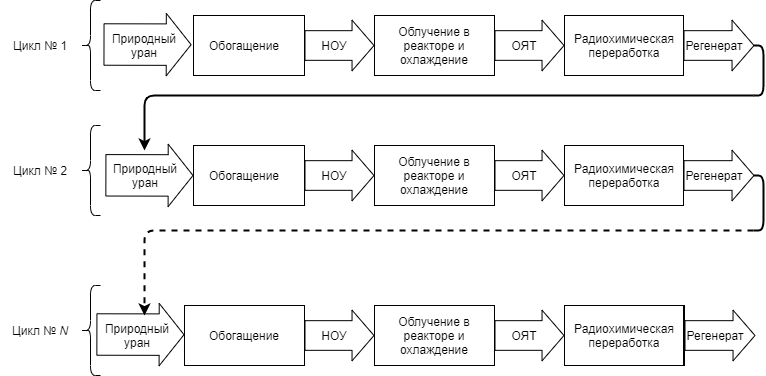
\includegraphics[scale=0.55]{theory/recycling_ru}}
  \caption{Схема многократного рециклирования урана}\label{recycle}
\end{figure}

\begin{figure}[ht]
  \centerfloat{
\includegraphics[scale=1.2]{cascades/ordinary/ordinary}}
  \caption{Схема ординарного трехпоточного каскада. $F$ -- поток питания; $P$ -- поток отбора; $W$ -- поток отвала.}\label{ordinary}
\end{figure}

В соответствии со схемой рис. \ref{recycle} предполагаем, что первичная загрузка реактора осуществлена топливом, изготовленном из обогащенного природного урана. Далее, при обогащении регенерированного урана природный уран используется в качестве материала подпитки, обеспечивающего необходимое количество дополнительного $^{235}$U для изготовления требуемой массы свежего топлива. Далее, процесс рецикла урана с добавлением природного сырья повторяют $N$ раз. Заметим, что материал подпитки необходим в рассматриваемой принципиальной схеме рецикла, так как в реакторе на тепловых нейтронах не достижимо расширенное воспроизводство ядерного топлива, из-за того, что коэффициент воспроизводства делящегося нуклида $^{235}$U в таком типе реакторов меньше единицы \cite{ignatevVliyanieVidaTopliva2020}. При этом очевидно, что природный уран является наиболее удобным материалом для добавлению к регенерату при производстве топлива новой загрузке. Тем не менее, вместо природного урана можно использовать и другие доступные урановые смеси, в которых либо очень низкая, либо нулевая концентрация четных изотопов. Например, это может быть НОУ с обогащением 1-1,5\%, обедненный уран и др.


Как следует из анализа результатов исследований, посвященных вопросам многократного рецикла урана в топливе легководных реакторов, в ходе рециклирования происходит рост (до нескольких раз) концентраций четных изотопов в регенерате после облучения в реакторе \cite{smirnovEvolutionIsotopicComposition2012}. При этом ввиду относительной малости концентрации $^{232}$U на первом (или, в некоторых случаях, на первых двух) рециклах не происходит достижения концентрацией этого изотопа предельных значений в финальном продукте \cite{smirnovApplyingEnrichmentCapacities2018}.
После роста концентраций четных изотопов на первых рециклах, наблюдается их постепенный выход на «плато», начиная с $\approx$3-го рецикла, что обусловлено фиксацией концентрации изотопа $^{232}$U в продукте на уровне $5\cdot10^{-7}$\%, что доказывает возможность многократного рециклирования облученной урановой топливной составляющей.

Таким образом, при анализе вопросов замыкания топливного цикла реакторов на тепловых нейтронах с использованием регенерированного урана необходимо учитывать такие факторы, как общая тенденция к повышению глубины выгорания в современных реакторах, так и рост концентраций четных изотопов в процессе рециклирования урана \cite{andrianovaPovyshenieVygoraniyaTopliva2008}. Это факторы делают актуальными разработку каскадных обогатительных схем, позволяющих эффективно использовать регенерированный уран при производстве товарного НОУ с учетом всех описанных выше требований и ограничений, в том числе, в условиях многократного рецикла урана.

Отметим ещё один важный фактор. Очевидно, что для извлечения максимальной выгоды из осуществляемой переработки ОЯТ, целесообразно максимально вовлекать в повторное использование весь выделенный из него регенерат. Это означает, что если рассматривать отдельный реактор, то логично при получении НОУ из регенерированного урана использовать при его производстве весь выделенный из ОЯТ этого же реактора регенерат. Это будет означать, во-первых, минимизацию потерь $^{235}$U в топливном цикле, во-вторых, максимально эффективное использование потенциала ОЯТ для воспроизводства топлива, а, в-третьих, отсутствие нежелательного накопления регенерата на складах. При этом следует сделать акцент на том, что подобное условие не является физическим требованием, а скорее призвано повысить эффективность замыкания топливного цикла реакторов на тепловых нейтронах по урановой составляющей. Схематично это условие иллюстрирует рисунок \ref{reconeto}.  

\begin{figure}[ht]
  \centerfloat{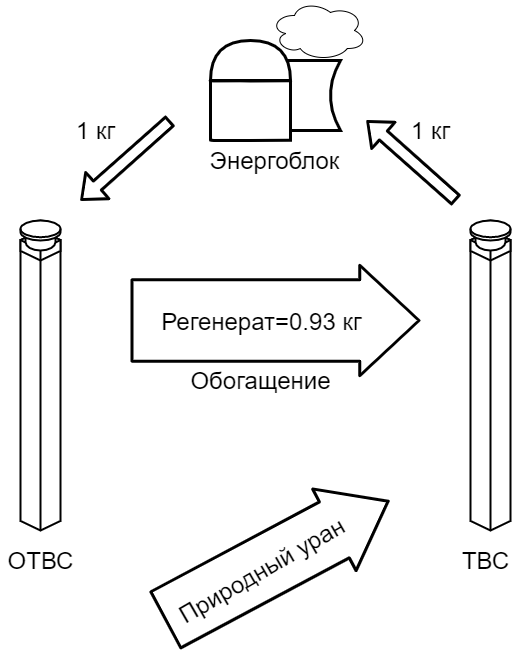
\includegraphics[scale=0.55]{theory/recycling1kg_ru}}
  \caption{Схема замыкания урановой топливной составляющей.}\label{reconeto}
\end{figure}


Учитывая сказанное выше, задача обогащения регенерата в общем случае может быть сформулирована как: получение заданной массы товарного НОУ требуемого обогащения по $^{235}$U из сырьевого регенерата урана (в том числе многократно рециклированного) с одновременным выполнением ограничений на концентрации четных изотопов при условии расходования всей массы регенерата, выделенного из ОЯТ данного реактора.

Таким образом, с обогащением регенерата урана в каскадах газовых центрифуг связаны определенные сложности, требующие модификации подходов, принятых на разделительных производствах при обогащении природного урана. Все перечисленные факторы обуславливают актуальность разработки в области поиска оптимальных каскадных схем для обогащения регенерированного урана с учетом требований, предъявляемых к получаемому продукту -- НОУ.

Оптимальность той или иной каскадной схемы зависит от выбранных критериев эффективности. В качестве таких критериев, как правило, используют минимум затрат работы разделения и расхода природного урана для получения единицы товарного НОУ. Эти характеристики в значительной мере определяют величину удельных затрат на получение товарного НОУ.


\section{Промышленный опыт}\label{sec:ch1/sec1}

Возврат урана в топливный цикл по представленной выше схеме опирается на три ключевые технологии:
\begin{enumerate}
  \item Радиохимическую переработку ОЯТ;
  \item Изотопное обогащение регенерированного урана;
  \item Изготовление топлива на основе восстановленного отработавшего топлива.
\end{enumerate}

Что касается первого пункта, в странах, лидирующих в развитии ядерных технологий, с середины прошлого века широко используется технология гидрометаллургической переработки облученного топлива, называемая PUREX \cite{selvaduraySurveyNuclearFuel1979}. В России, технологии связанные с переработкой ОЯТ развиваются особенно успешно благодаря ориентированности отрасли на замыкание ЯТЦ \cite{balihinSostoyaniiPerspektivahRazvitiya2018, efimenkoProblemyPerspektivyRazvitiya2017}. В виду такого стратегического курса отечественной атомной отрасли, запланирован ввод новых мощностей, которые расчитаны на переработку принимаемого ОЯТ из-за рубежа \cite{050519L3942005}. С 2016 г. на <<ФГУП ПО <<МАЯК>> осуществляется переработка партий ОТВС ВВЭР-1000 \cite{PyatyyNacionalnyyDoklad}.

Что касается технологии изотопного обогащения урановых смесей, российская атомная промышленность имеет опыт обогащения регенерированного урана из реакторов ВВЭР-440, который затем использовался в качестве топлива РБМК \cite{VVER10001200Za}. Для этого используют метод прямого обогащения в трехпоточной каскадной схеме. Такая схема реализована для производства исходного сырья для изготовления топлива РБМК на заводе РТ-1 \cite{volkVozvratUranaIz2010}. Этот вариант также апробирован для изготовления опытных тепловыделяющих сборок (ТВС) для реакторов ВВЭР, требующих более высокого уровня обогащения \cite{proselkovAnalizVozmozhnostiIspolzovaniya2003}.
% Здесь важно также отметить, что на сегодняшний день у топливного дивизиона Росатома имеется уникальный технологический задел, связанный с газоцентрифужной технологией, который уже сегодня отражен в доминирующей роли этой технологии на мировом рынке разделительных услуг за счет низкой себестоимости единицы работы разделения, которую обеспечивают энергоэффективные и долговечные разделительные аппараты.

Что касается заключительного пункта, Росатом на одном из заводов фабрикации ядерного топлива осуществлял изготовление опытных образцов тепловыделяющих сборок в том числе на основе зарубежного облученного топлива (из Франции) с повышенным содержанием $^{232}$U \cite{kislovRadiacionnyeAspektyIspolzovaniya}.

Имеющийся в России опыт рециклирования ядерного топлива базируется на смешении регенератов урана, извлекаемых из ОЯТ ВВЭР и ОЯТ транспортных реакторов с высоким содержанием $^{235}$U \cite{international2003iaea}.

При этом зарубежный опыт базируется на однократном использовании MOX-топлива \cite{international2003iaea}.

% При этом, опираясь на передовой уровень разделительной технологии, можно заключить, что задача обогащения регенерата до необходимого для повторного использования в энергетических ядерных реакторах уровня концентрации изотопа $^{235}$U может быть решена.

Таким образом, сложившаяся к текущему моменту в России научно-производственная база с наращиваемыми объемами промышленных разделительных мощностей, основанных на центробежном методе разделения, является основным аргументом в пользу готовности к вовлечению регенерата в топливный цикл легководных реакторов.

Однако, для практической реализации долгосрочных планов отрасли по замыканию ЯТЦ и расширению предложения международных топливных поставок, что предусматривает многократное рециклирование делящихся материалов, необходимо решить задачу возврата регенерата в ЯТЦ, подразумевая наличие вышеизложенных ограничений \cite{RosatomGoskorporaciyaRosatoma,panteleyOsobennostiMezhdunarodnogoSotrudnichestva2017}.

Для анализа возможности решения задачи рецикла урана в рамках поставленных ограничений с помощью ранее предложенных схем, перейдем к их подробному рассмотрению.

\section{Обзор способов обогащения регенерата урана в каскадах центрифуг}

Ниже приведены результаты критического анализа основных из предложенных к настоящему моменту каскадных схем, что позволяет охарактеризовать их достоинства и недостатки,  и сделать вывод о возможности их использования для решения задачи обогащения регенерата урана в условиях его многократного рецикла в топливе современных реакторов на тепловых нейтронах.

Принимая во внимание сложность сформулированной выше задачи обогащения регенерата по отношению к случаю обогащения природного урана, непосредственное применение штатной схемы обогащения -- ординарного или трехпоточного каскада имеет существенные ограничения и в общем случае поставленную задачу не решает. Главная причина состоит в том, что подобный каскад имеет всего один выходящий поток отбора, в котором, одновременно будут концентрироваться, как целевой  $^{235}$U, так и четные изотопы. В результате ординарный каскад позволяет лишь обогащать относительно «чистые» составы регенерата, в которых исходные содержания четных изотопов меньше (на порядок или более), чем их допустимые пределы в товарном НОУ. Однако эти условия, очевидно, невыполнимы при многократном рецикле урана.
Проведенные сравнительный анализ предложенных способов обогащения регенерата позволяет условно разделить их на 3 типа: схемы с разбавлением четных изотопов,  схемы с отделением четных изотопов, «гибридные» схемы. 
Ниже проанализированы каскадные схемы каждого из указанных типов. В Приложении представлены результаты тестовых расчётов обогащения регенерата различного исходного состава для большинства рассмотренных ниже схем с целью оценки их эффективности для решения поставленной задачи.

\subsection{Каскадные схемы с разбавлением четных изотопов}

Ряд из предложенных каскадных схем обогащения регенерата в качестве основного фактора, корректирующего изотопный состав регенерата в процессе его обогащения, используют разбавление четных изотопов урановой смесью, которая их не содержит. В качестве таких разбавителей чаще всего рассматривают природный уран, однако это могут быть также обедненный или низкообогащенный уран.

Простейшие схемы с разбавлением основаны на использовании штатного ординарного каскада. Рассмотрим такие схемы, которые могут быть реализованы следующими способами (рис. \ref{fig:diagram1}) \cite{sulaberidzeNekotoryhRazdelitelnyhProblemah2004,smirnovKaskadnyeShemyZadachah2012}:

\begin{enumerate}
  \item Смешивание регенерированного урана и природного (или обедненного) урана перед подачей в каскад рис. (рис. \ref{fig:diagram1}.1).
  \item Получение обогащенной фракции из регенерата и последующее ее разбавление природной урановой смесью (рис. \ref{fig:diagram1}.2).
  \item Получение НОУ из природного урана путем его прямого обогащения, с последующим разбавлением регенератом (рис. \ref{fig:diagram1}.3).
\end{enumerate}

\begin{figure}[ht]
  \centerfloat{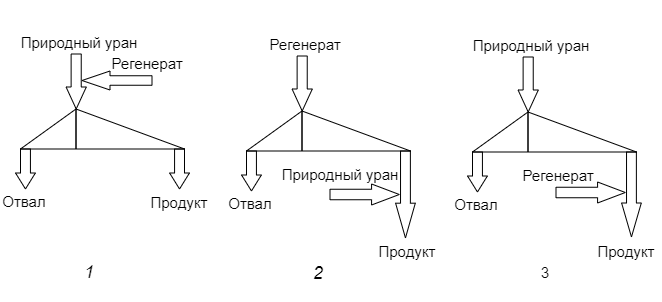
\includegraphics[scale=0.7]{cascades/diagram1}}
  \caption{Схемы на основе ординарного каскада}\label{fig:diagram1}
\end{figure}

Для всех вариантов схем рис. \ref{fig:diagram1} сотношение между расходом регенерата и разбавителем природного происхождения определяется пределом допустимой концентрации $^{232}$U в конечном продукте -- низкообогащенном уране. Также компенсируется отрицательная реактивность $^{236}$U с помощью добавочной концентрации $^{235}$U к той, что требуется для НОУ-топлива с заданными свойствами.

Основным преимуществом таких схем является простота реализации, поскольку нет необходимости в модификации самого каскада, так как операции разбавления осуществляются за его пределами.

В качестве недостатков таких схем можно выделить:
\begin{enumerate}
  \item отсутствие возможности очищать регенерированный уран от четных изотопов, так как такие схемы основаны исключительно на разбавлении четных изотопов до допустимых концентраций;
  \item потери работы разделения, возникающие из-за смешения потоков с различными изотопными концентрациями $^{235}$U;
  \item невозможность выполнения условия «полного использования регенерированного урана» при многократном рецикле \cite{smirnovApplyingEnrichmentCapacities2018} (см. Приложение/глава 3);
  \item выполнение ограничений по концентрации $^{232}$U в продукте напрямую зависит от концентрации указанного изотопа в поступившем на обогащение регенерате;
  \item для схем рис. \ref{fig:diagram1}.1--\ref{fig:diagram1}.2 имеет место загрязнение 100\% задействованных в обогащении регенерированного урана разделительных мощностей, что делает проблематичным их дальнейшее «перепрофилирование» на обогащение природного урана, по крайней мере в случае длительной (в течение нескольких лет) работы с регенерированным ураном.
\end{enumerate}

Подытоживая рассмотрение простейших разбавляющих схем обогащения регенерата можно отметить, что их использование не позволяет очищать регенерат от чётных изотопов, вся масса которых в значительной мере переносится в отбор каскада, что затрудняет использование таких схем в условиях многократного рецикла, когда концентрации чётных изотопов возрастают. Поэтому такие каскадные схемы потенциально применимы только для обогащения относительно «чистого» состава регенерата, в котором содержание $^{232}$U меньше допустимой нормы на порядок и более, что нехарактерно для изотопных составов выгружаемого из активной зоны современных ВВЭР облученного топлива при многократном рецикле урана \cite{bormanTehnikoekonomicheskiyAnalizVozmozhnyh2012}. 

Другие варианты каскадных схем с разбавлением чётных изотопов основаны на использовании так называемых многопоточных каскадов \cite{sulaberidzeQuasiidealCascadesAdditional2006}. В отличие от предыдущих вариантов в рассматриваемом случае разбавление регенерата осуществляют непосредственно в каскаде путем подачи одного или нескольких разбавителей в качестве дополнительного питания каскада параллельно с самим регенерированным ураном. Подобное разбавление одним или несколькими разбавителями можно осуществить в каскадах с двумя или тремя внешними питаниями (рисунки \ref{fig:2_inputs}, \ref{fig:3_inputs}).

\begin{figure}[ht]
  \centerfloat{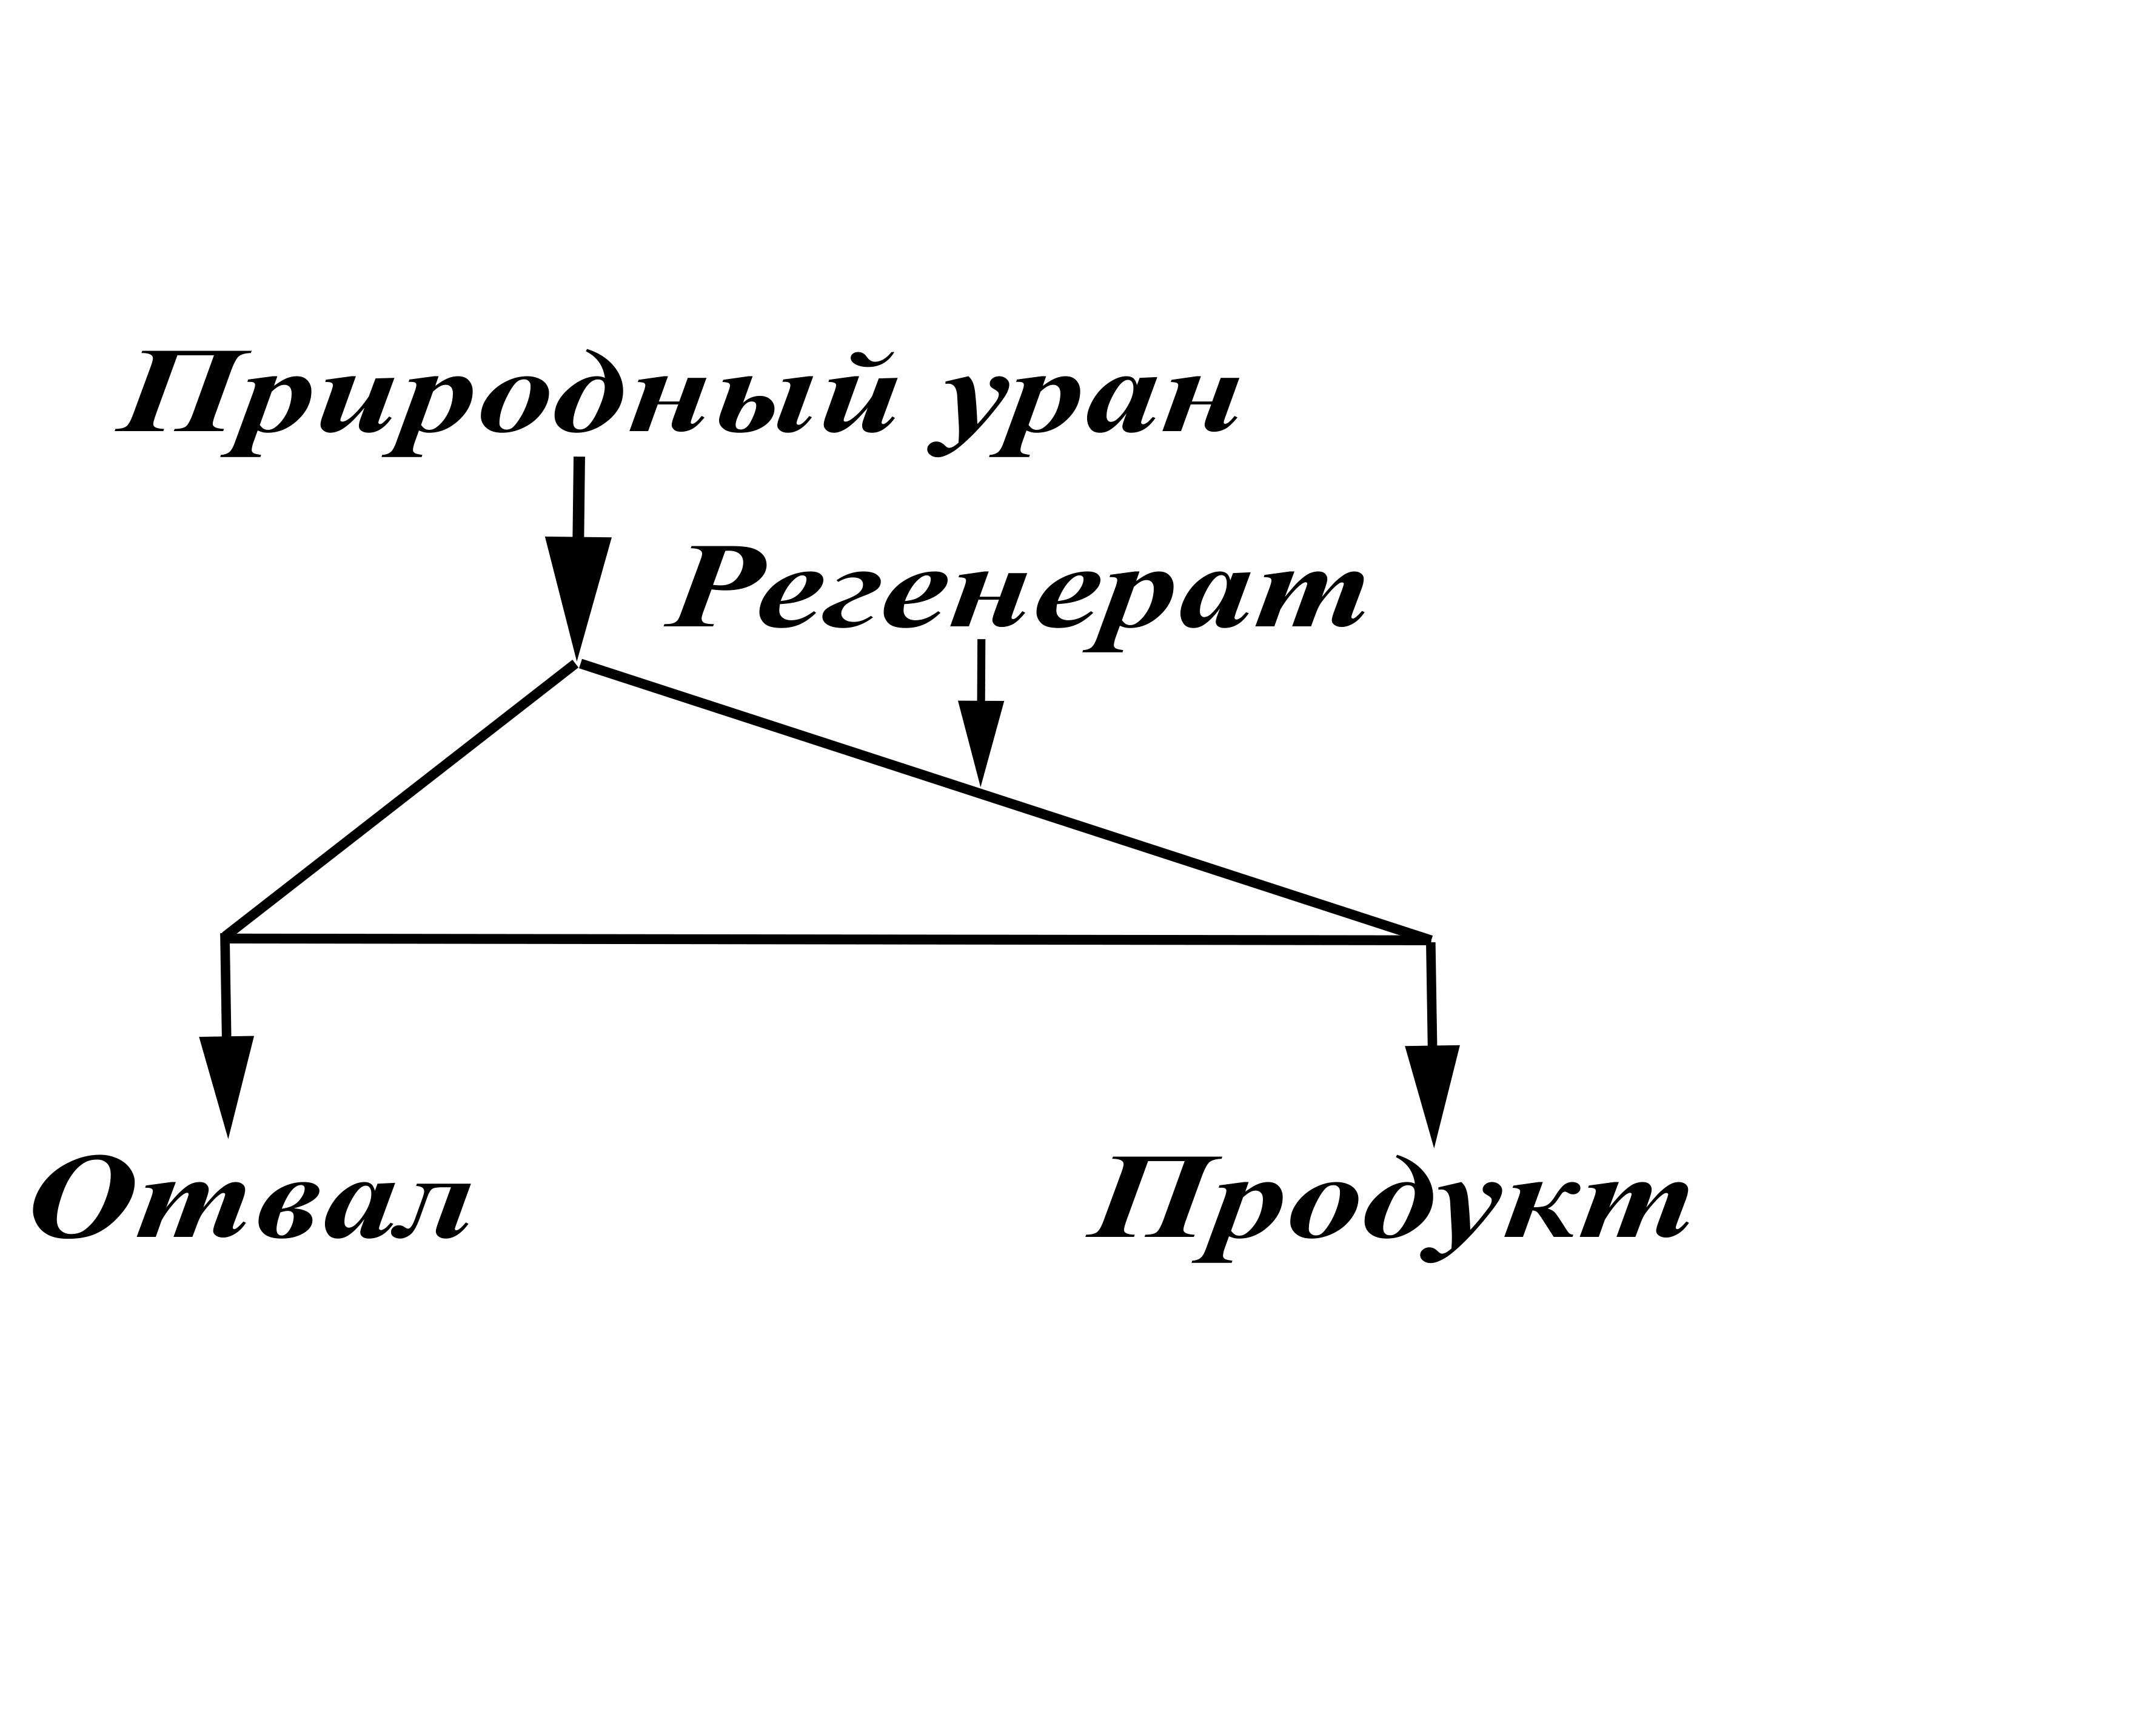
\includegraphics[scale=0.07]{cascades/2in}}
  \caption{Каскад с дополнительным потоком питания}\label{fig:2_inputs}
\end{figure}

\begin{figure}[ht]
  \centerfloat{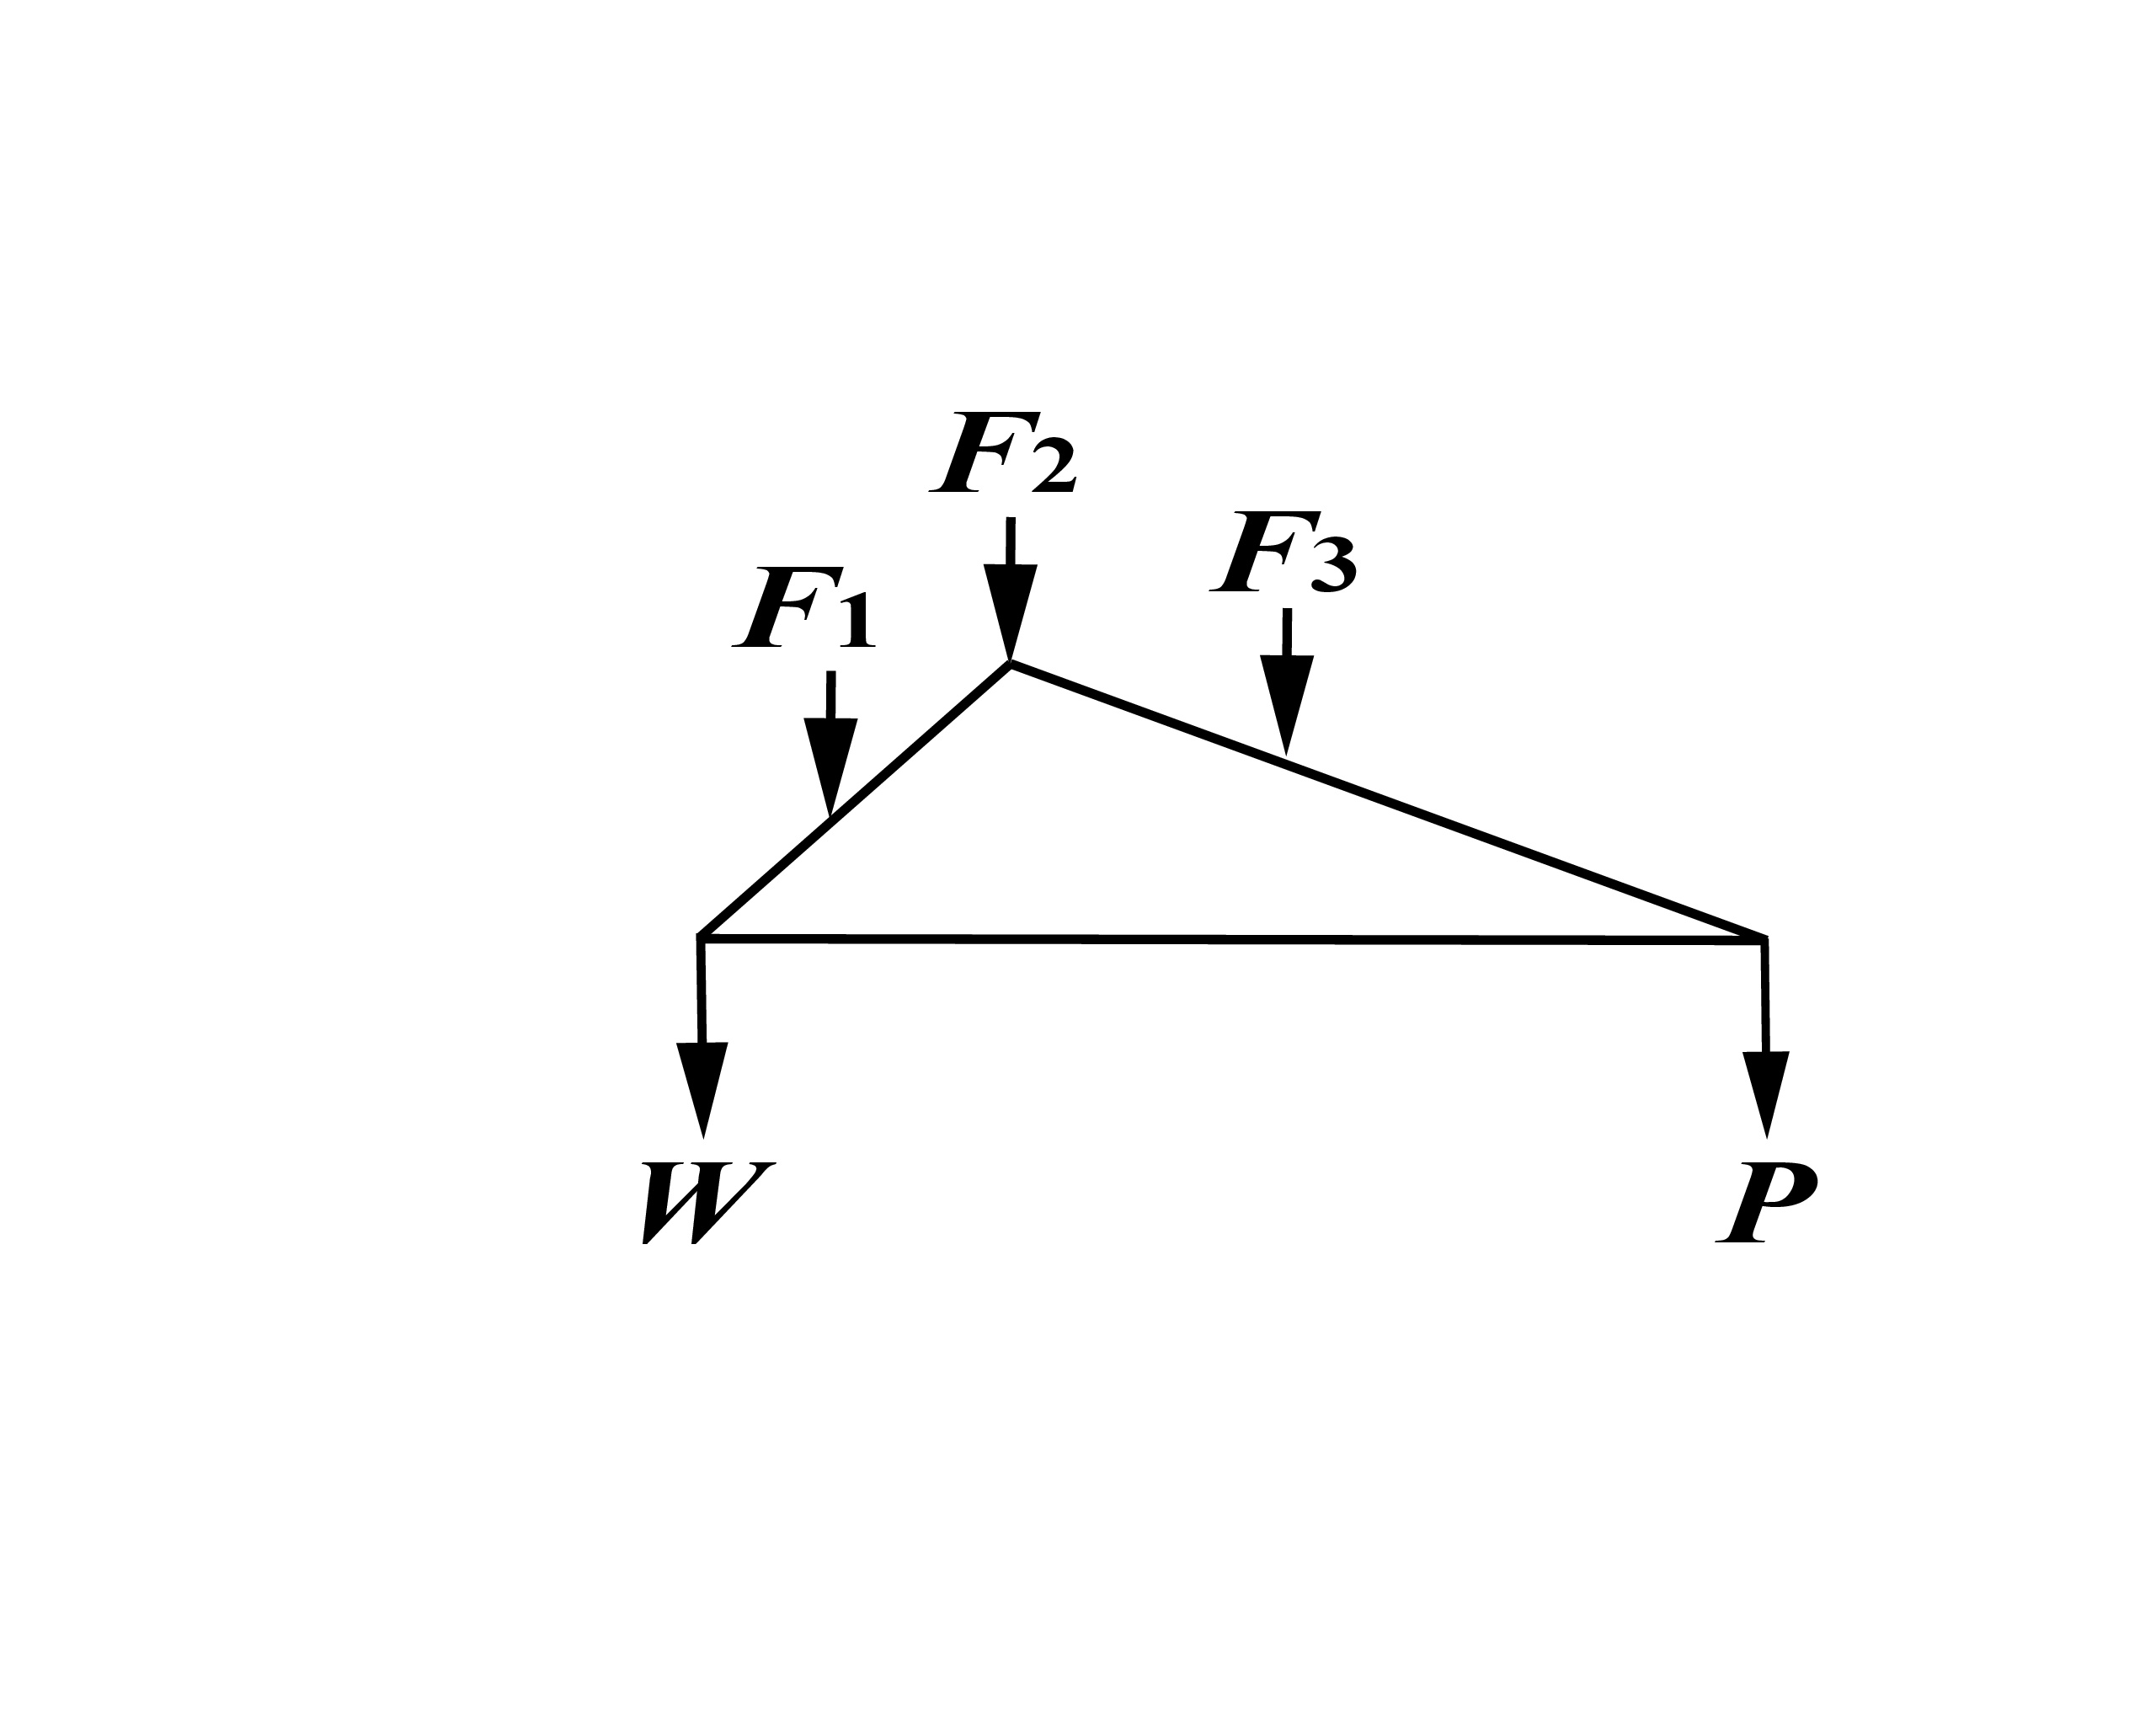
\includegraphics[scale=0.17]{cascades/3in}}
  \caption{Каскад с тремя потоками питания}\label{fig:3_inputs}
\end{figure}

Ключевые отличие от рассмотренных выше схем на основе ординарного каскада в этих случаях состоит в том, что разбавление регенерата происходит непосредственно внутри каскада. При этом подача разбавителя(лей) в каскад в виде дополнительных потоков питания преследует цель минимизации потерь работы разделения при смешивание потоков с различным содержанием изотопа $^{235}$U. Это достигается за счет подачи потоков регенерированного урана и разбавителя в ступени каскада с близкими концентрациями изотопа $^{235}$U.
На рисунке \ref{fig:2_inputs} изображен вариант каскада с двумя питаниями: обогащаемый регенерированный уран, разбавитель -- природный уран. Как следует из результатов исследования \cite{smirnovEvolutionIsotopicComposition2012} в условиях многократного рецикла в топливе ВВЭР данная схема не способна обеспечить выполнение условия «полного использования регенерата», начиная со второго или третьего рецикла в зависимости от заданной величины допустимой концентрации $^{232}$U в товарном НОУ ($2\cdot10^{-7}$\% или $5\cdot10^{-7}$\%).

Схема, представленная на рисунке \ref{fig:2_inputs} является чуть более сложной, но также является разбавляющей. Основное отличие от предыдущего варианта состоит в том, что разбавление регенерированного урана осуществляют с использованием комбинации разбавителей \cite{smirnovObogashchenieRegenerirovannogoUrana2014}. В одном из вариантов наряду с природным ураном для разбавления в каскад подают обедненный уран. В других случаях, наоборот, природный уран может быть заменен НОУ с обогащением 1,0--2,0\% \cite{smirnovObogashchenieRegenerirovannogoUrana2017}.

Использование комбинации разбавителей позволяет при заданных требованиях к продукту варьировать ключевые интегральные характеристики схемы: удельный расход природного урана и затраты работы разделения при получении товарного НОУ. Однако как и в случае с другими разбавляющими каскадными схемами при увеличении исходных концентраций четных изотопов в регенерате эффективность рассматриваемых схем с дополнительными питаниями снижается, а начиная с определенных концентраций $^{232}$U подобные схемы не могут обеспечить условие полного использования регенерата, тем самым не решая сформулированную выше в общем случае задачу обогащения регенерата. Ключевая причина снижения эффективности состоит в том, что данная схема, как и все предыдущие варианты имеет лишь один выводной поток, обогащенный по легким компонентам. В этом потоке неминуемо одновременно с целевым изотопом $^{235}$U концентрируются и все четные изотопы, включая $^{236}$U. Таким образом, комбинирование разбавителей лишь дает возможность варьировать расходные характеристики схемы, но не корректировать изотопный состав получаемого продукта.
Невозможность решения задачи обогащения регенерированного урана произвольного состава в разбавляющих каскадных схемах легко проиллюстрировать аналитической оценкой, основанной на условии баланса материальных потоков в каскаде. 
Как известно, в стационарном режиме работы, в отсутствии потерь или источников рабочего вещества, внешние параметры ординарного каскада подчиняются следующим условиям, выражающим закон сохранения вещества \cite{sulaberidzeTeoriyaKaskadovDlya2011}:


Как известно, в стационарном режиме работы, в отсутствии потерь или источников рабочего вещества, внешние параметры ординарного каскада подчиняются следующим условиям, выражающим закон сохранения вещества:
				  
\begin{equation} \label{EQ__1} 
  \begin{array}{l} {\quad \quad \quad \quad F=P+W,} \\ {FC_{i}^{F} =PC_{i}^{P} +WC_{i}^{W} ,\; i=1,2,...,m.} \end{array} 
\end{equation} 


где F -- поток питания каскада, P -- поток отбора каскада, W -- поток отвала каскада, $C_{i}^{F}$, $C_{i}^{P}$, $C_{i}^{W}$, -- концентрации i-го компонента в потоках F, P и W, соответственно, m -- число компонентов разделяемой смеси.

В случае, если регенерат подают в каскад совместно с разбавителем (например, природным ураном), независимо от способа его подачи в каскад выполняется следующее соотношение, выражающее закон сохранения i-го компонента смеси:

\begin{equation} \label{EQ__2} 
  \begin{array}{l} {FC_{i}^{F}+F_{nat.}C_{i}^{F_{nat.}} =PC_{i}^{P} +WC_{i}^{W} ,\; i=1,2,...,m.} \end{array} 
\end{equation} 

где Fnat -- поток природного урана с концентрациями компонентов , которые равны нулю для изотопов $^{232}$U, $^{233}$U, $^{236}$U. Следует отметить, что $^{233}$U является еще одним искусственным изотопом урана, однако его присутствие не оказывает негативного влияния на характеристики НОУ. Напротив, его свойства близки к $^{235}$U, но в силу малости его содержания (на уровне $10\cdot10^{-8}$--$10\cdot10^{-7}$\%), данным фактором можно пренебречь.

Довольно очевидно, что изотоп $^{232}$U, как наиболее легкий в разделяемой смеси, будет наиболее интенсивно обогащаться в отборе каскада и обедняться в его отвале. При этом для стандартных значений концентраций $^{235}$U в отвале каскада (0,1--0,2\%) для концентрации 232U в этом потоке будет справедливо условие  (индекс «1» соответствует изотопу $^{232}$U). Учитывая условие W$\textless$F, из соотношения \ref{EQ__2} легко получить следующее:

\begin{equation}\label{EQ_4} 
  \begin{array}{l} {C_{232}^{\mathrm{P}} \approx \frac{\mathrm{F}}{\mathrm{P}} \mathrm{C}_{232}^{\mathrm{F}}} \end{array}
\end{equation}

Из соотношения \ref{EQ_4} следует, что если необходимо выполнить условие «полного использования регенерата» и обеспечить величину $\frac{F}{P}\approx$ 0,95, что характерно для случая возврата регенерата из ОЯТ реакторов ВВЭР, то величина концентрации  может быть только больше соответствующего значения в исходном регенерате. По этой причине с использованием «разбавляющих» схем каскадов возможно обогащение только некоторых составов регенерата, соответствующих малым (до 40 МВт сут/кг) глубинам выгорания топлива и характеризующихся приемлемым исходным содержанием изотопа $^{232}$U.

Однако для современных величин глубины выгорания топлива, концентрация $^{232}$U даже в исходном регенерате может изначально превосходить величину ограничения. Например, это характерно для многократно рециклированного урана. Изменить эту ситуацию невозможно ввиду отсутствия параметров, позволяющих уменьшать относительную концентрацию изотопов $^{232}$U и $^{235}$U одновременно с обогащением последнего (и здесь и далее под относительной концентрацией компонентов понимаем отношение их абсолютных массово-долевых концентраций).

Проделанный анализ показывает, что выполнение условия «полного использования регенерата» возможно только, если концентрация $^{232}$U в исходном регенерате не превышает требуемого ограничения на выходе из каскада. Это может оказаться невыполнимым условием для случая многократного рецикла урана в топливе ВВЭР, при котором концентрация $^{232}$U в исходном регенерате, как правило, превышает допустимые ограничения уже начиная со второго рецикла. Данное обстоятельство фактически делает невозможным использование любого из описанных выше вариантов разбавляющих схем для решения сформулированной выше задачи обогащения регенерата урана в условиях многократного рецикла.



Помимо описанных выше вариантов разбавляющих каскадных схем, предложены и более сложные подходы, позволяющие с оговоркой получить очищенный регенерированный уран. Эффект очистки состоит в том, что в таком способе возможно получить регенерированный уран с концентрацией $^{235}$U, как в исходной смеси, но существенно сниженным содержанием четных изотопов. Пример такой каскадной схемы представлен на рисунке \ref{fig:3_out}. Она представляет собой каскад с дополнительными питанием и дополнительным отбором \cite{palkinSeparationUraniumIsotopes2010}. Основным питанием каскада выступает разбавитель, в предложенном варианте - природный уран. Дополнительным питанием выступает обогащаемый регенерат. В отборе на конце такого каскада получают поток НОУ товарного качества. Поток дополнительного отбора представляет собой «очищенный» от чётных изотопов регенерат. Из полученного в дополнительном отборе полупродукта в дальнейшем может быть наработан товарный НОУ, для чего схему надо будет модифицировать, добавив еще один каскад.

\begin{figure}[ht]
  \centerfloat{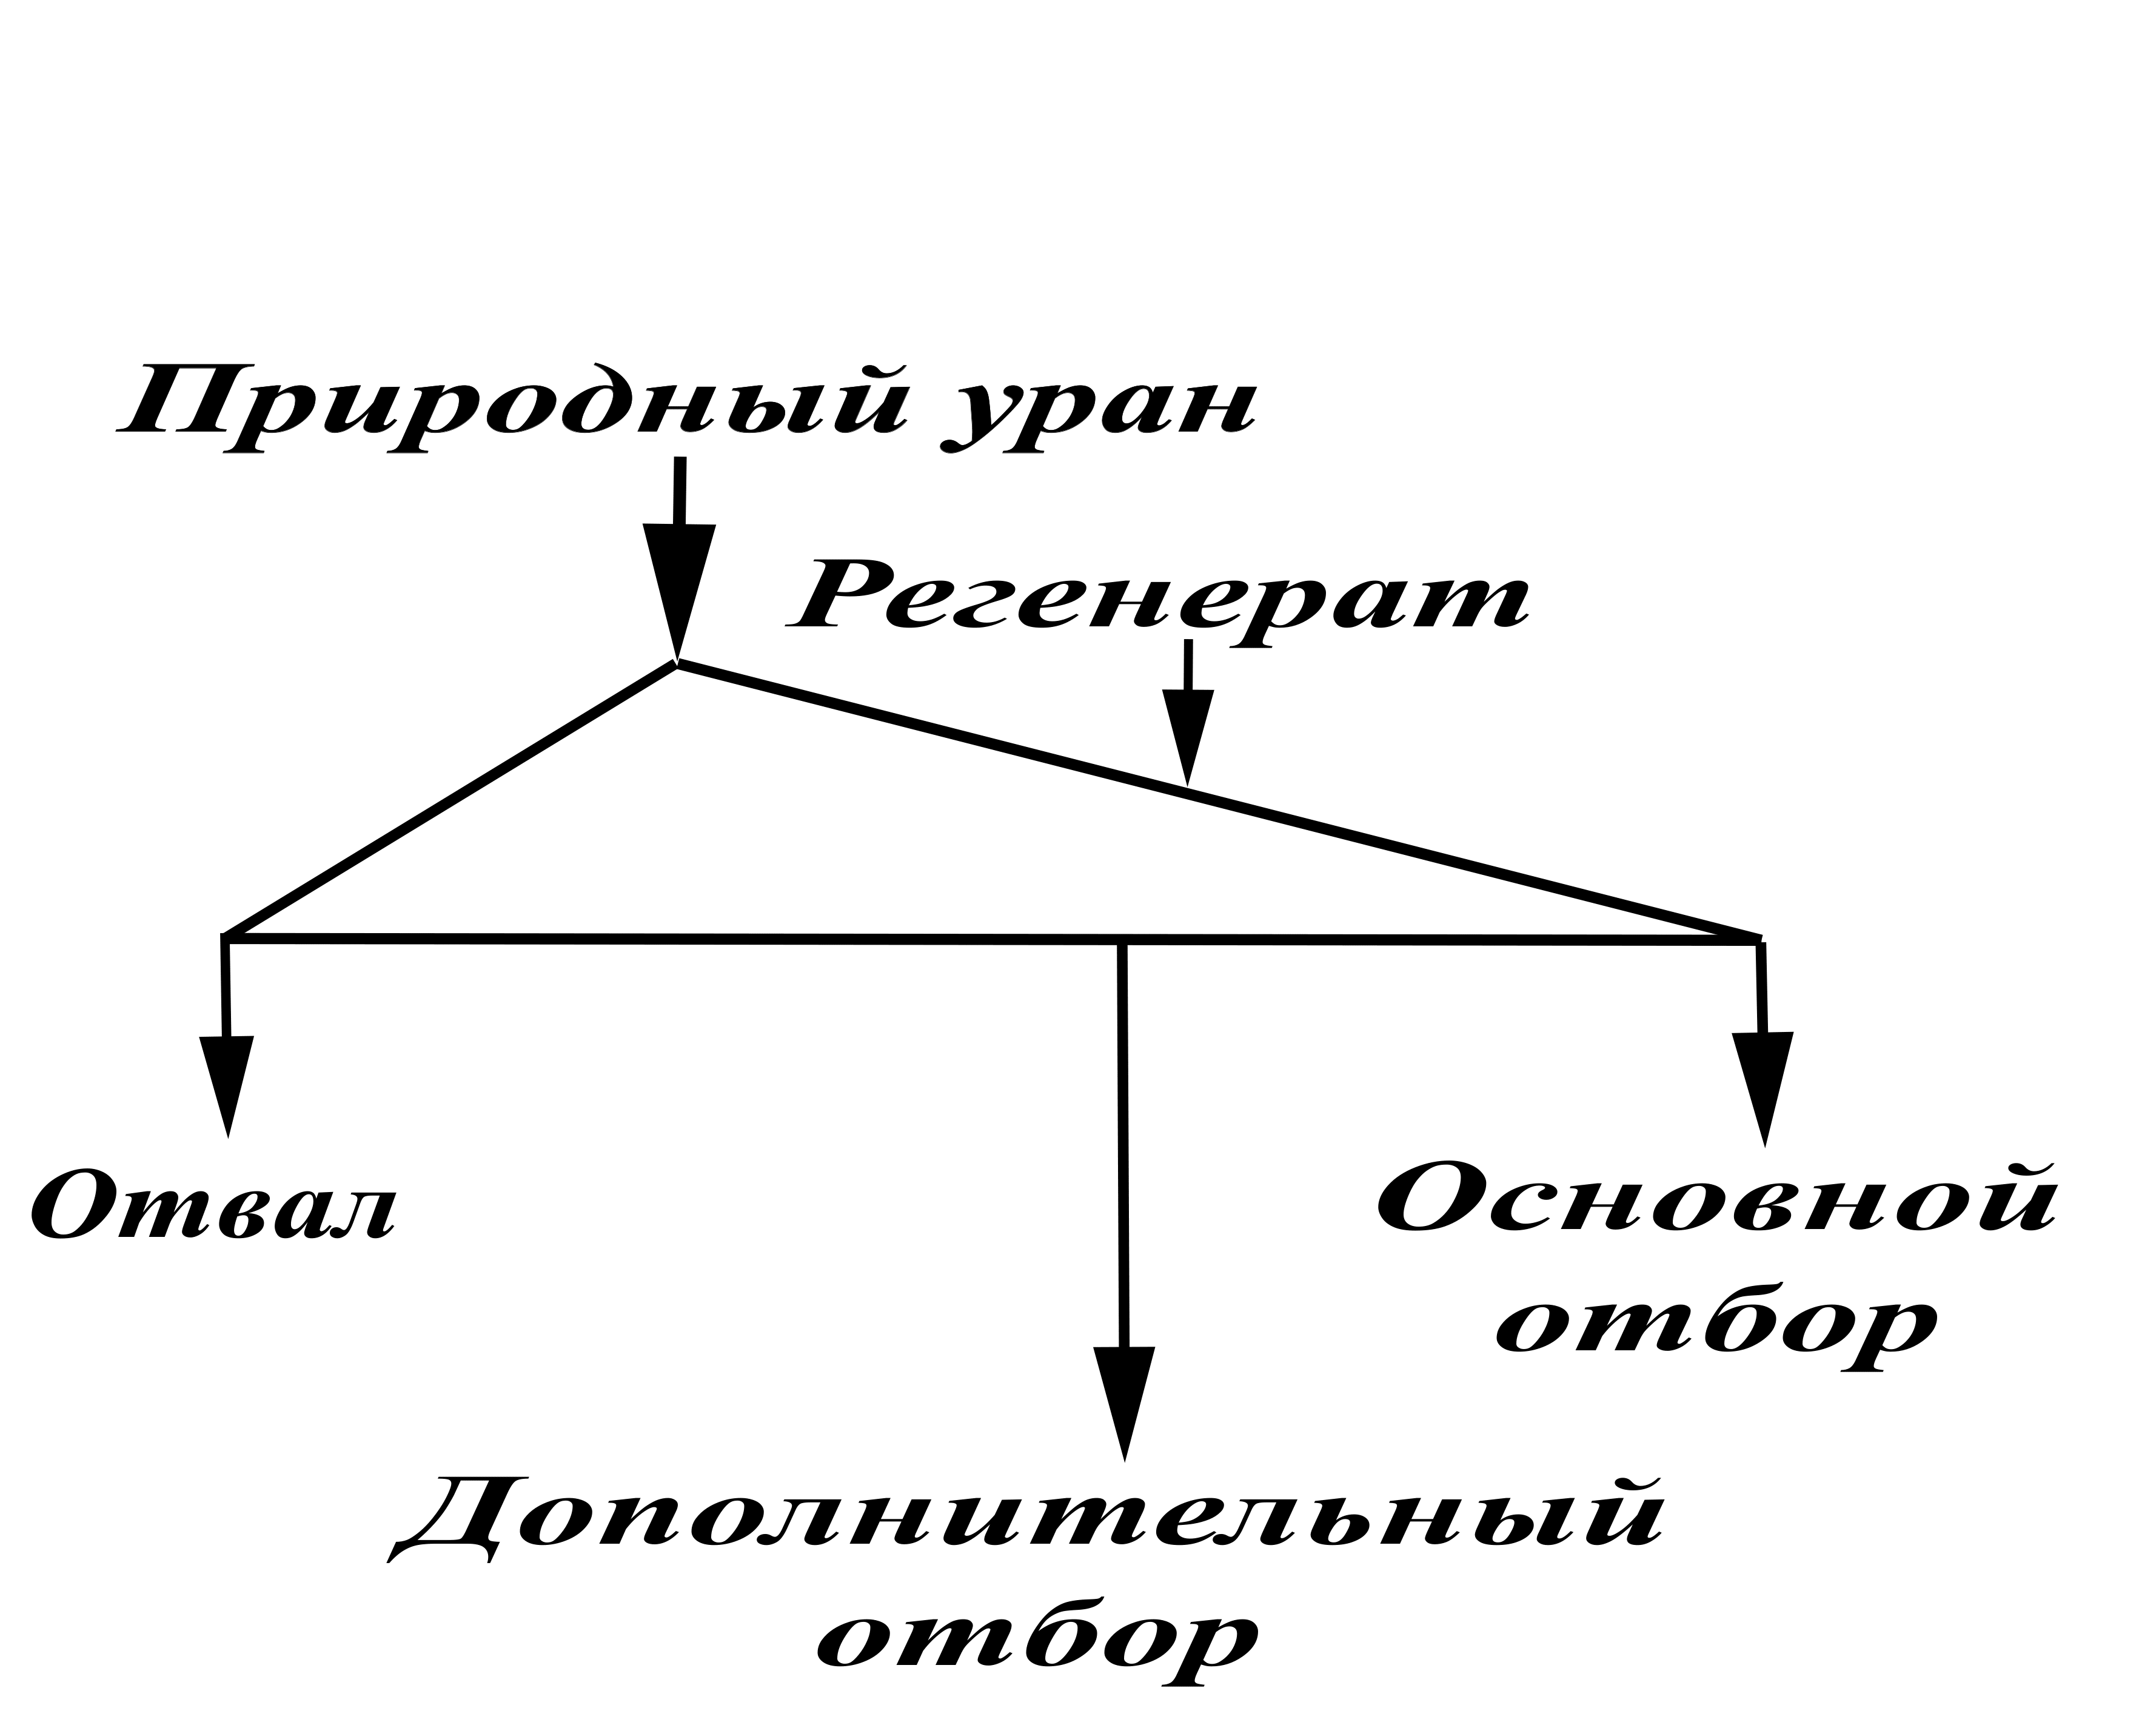
\includegraphics[scale=0.07]{cascades/3out}}
  \caption{Каскад с дополнительным потоком отбора для очистки регенерированного урана от минорных изотопов}\label{fig:3_out}
\end{figure}

По существу своей работы представленная на рисунке \ref{fig:3_out} каскадная схема является модификацией рассмотренной ранее схемы с двумя потоками питания. Отличие заключается в наличии потока дополнительного отбора, в котором получают очищенный регенерат. Однако наличие этого потока накладывает определенные ограничения на соотношения между потоками природного урана и регенерата, поступающих в каскад. Это обусловлено тем, что заметного снижения содержания минорных изотопов в дополнительном отборе можно добиться лишь при значительном разбавлении регенерата природным сырьем, в соотношениях, лежащих в диапазоне (1-25)/100 \cite{palkinSeparationUraniumIsotopes2010,smirnovKaskadnyeShemyZadachah2012}. Фактически это означает, что основной эффект «очистки» здесь также обусловлен разбавлением и включением дополнительного отбора на ступени с концентрацией $^{235}$U, близкой к таковой в исходном регенерате. При этом в схеме не происходит фактического отделения $^{235}$U от четных изотопов. Важно также отметить, что в представленных в \cite{palkinSeparationUraniumIsotopes2010} расчётных примерах эффективность такой схемы проверяли на примере состава регенерата с относительно невысоким содержанием изотопа $^{232}$U. ПРоведенные в рамках настоящей работы тестовые расчёты на примере обогащения регенерата пятого рецикла показали её неспособность решить в общем случае задачу обогащения регенерата, что затрудняет использование такой схемы для его многократного рецикла (см Приложение 1).

Таким образом, рассматриваемая каскадная схема не может обеспечить решение сформулированной выше задачи обогащения регенерата в условиях многократного рецикла по тем же причинам, по которым подобную задачу не решают и другие «разбавляющие» схемы. Отдельного анализа требует также вопрос использования получаемого в дополнительном отборе очищенного регенерированного урана. В зависимости от входящего состава обогащаемого регенерированного урана данный материал может быть не пригоден для последующего прямого обогащения в ординарном каскаде, что ставит под сомнение целесообразность получения такого материала в принципе.
Подытоживая проведенный краткий анализ способов обогащения регенерата, основанных на его разбавлении, отметим их общие достоинства и недостатки.

К достоинствам подобных схем можно отнести следующее:

\begin{enumerate}
  \item	позволяют снижать концентрацию четных изотопов при обогащении регенерата различного исходного состава;
  \item	относительная простота реализации на основе центробежного метода разделения;
  \item	в большинстве вариантов реализации «разбавляющие» схемы позволяют осуществить процесс обогащения без превышения допустимых концентраций четных изотопов на отдельных ступенях каскада.
\end{enumerate} 

К недостаткам «разбавляющих» схем можно отнести следующее:

\begin{enumerate}
  \item	эффект снижения концентрации четных изотопов в таких схемах связан преимущественно с их разбавлением продуктами, не содержащими четных изотопов (природный уран, обедненный уран, НОУ из природного урана), что делает невозможным решение сформулированной выше задачи обогащения регенерированного урана в условиях многократного рецикла урана в топливе современных реакторов на тепловых нейтронах;
  \item	 для большинства вариантов разбавляющих схем происходит загрязнение 100\% разделительного оборудования, что может затруднить последующее его использование для обогащения смесей урана, не содержащих изотопов $^{232}$U и $^{236}$U.
\end{enumerate}

Описанные выше недостатки «разбавляющих» схем стимулировали развитие иных подходов к обогащению регенерированного урана, которые описаны ниже.



\subsection{Схемы с очисткой от $^{232}$U. Двойные каскады}

Простейшим вариантом каскада, реализующим отделение $^{232}$U от $^{235}$U в процессе обогащения регенерата является двойной каскад -- последовательное соединение двух каскадов (рис. \ref{fig:double_ru}). 

\begin{figure}[ht]
  \centerfloat{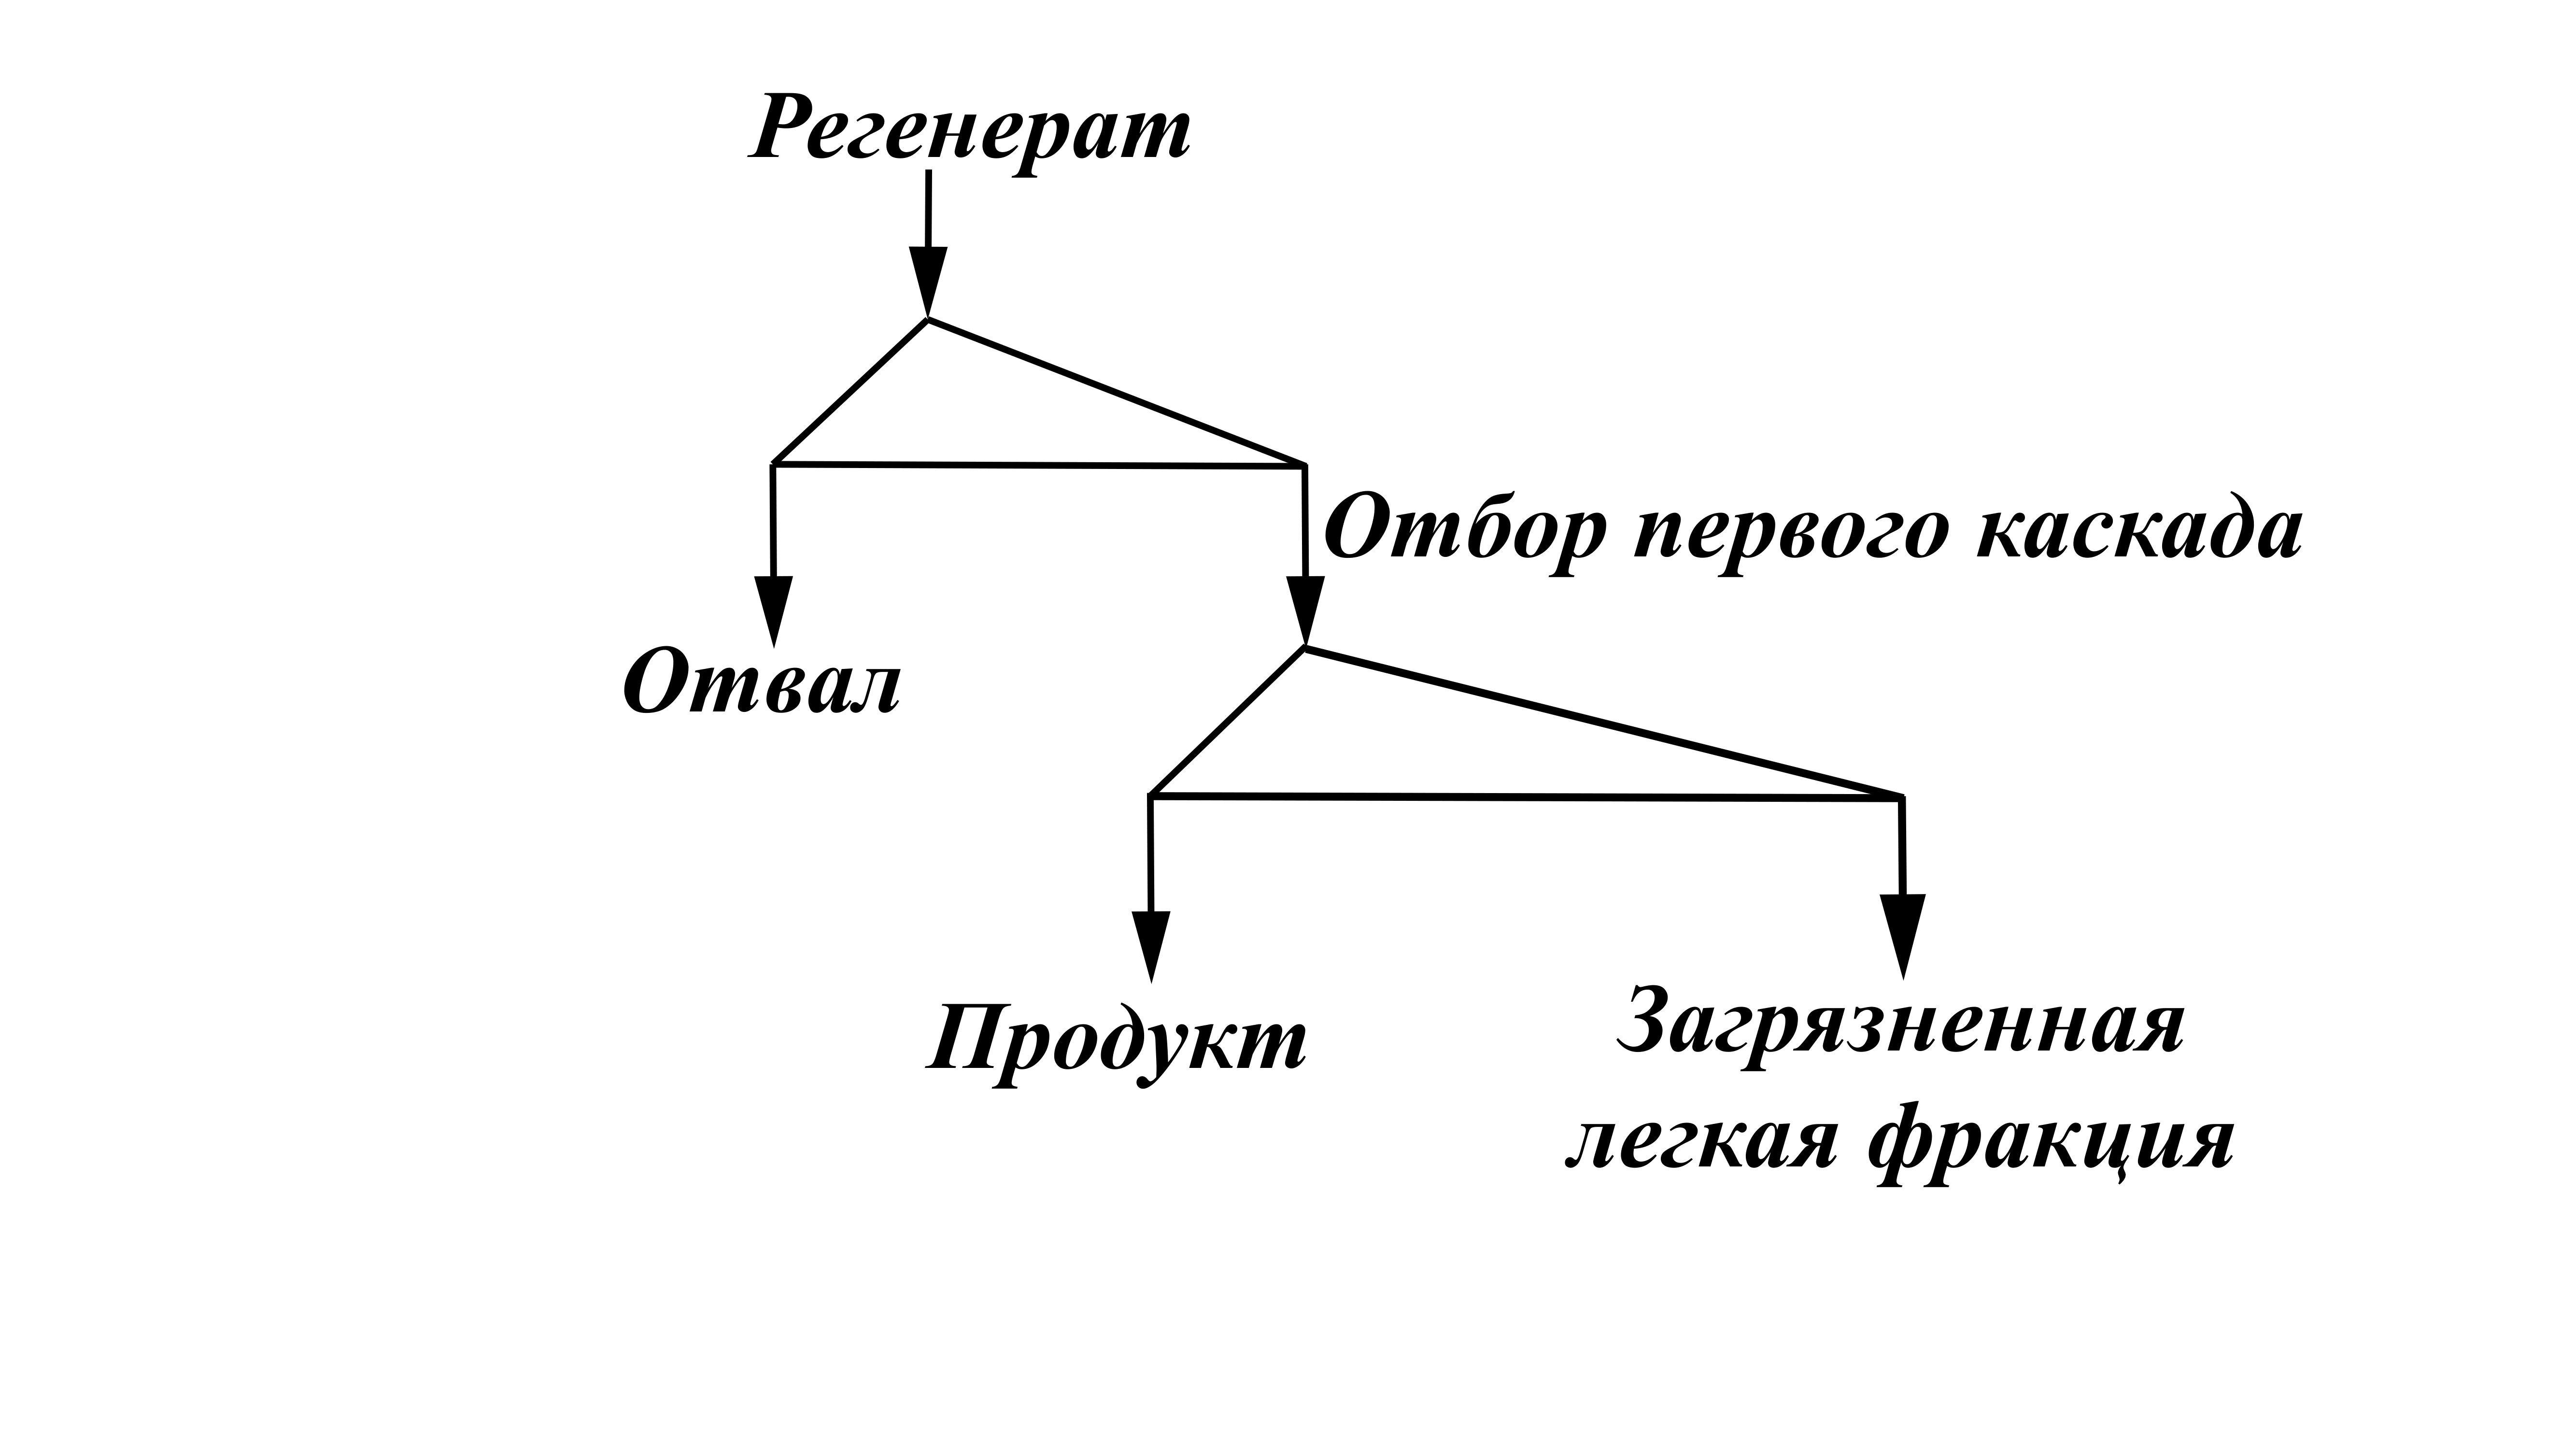
\includegraphics[scale=0.07]{cascades/double_ru}}
  \caption{Двойной каскад}\label{fig:double_ru}
\end{figure}

Подобные каскадные схемы можно условно назвать «очищающими» от чётных изотопов. Идея работы подобных каскадов заключается в том, чтобы сконцентрировать нежелательные четные изотопы отдельно от целевого изотопа -- $^{235}$U. В отличие от рассмотренных выше схем с разбавлением четных изотопов в данном случае действительно может быть реализована очистка от них (хотя бы частично).

В простейшем варианте  реализации отделение четных изотопов от $^{235}$U может быть осуществлено следующим образом. Сначала, в первом каскаде обогащают изотоп $^{235}$U с одновременным обогащением изотопов $^{232}$U, $^{234}$U и $^{236}$U, затем полученную смесь направляют на вход второго каскада, где она делится на две группы: в первой обогащены легкие изотопы ($^{232}$U, $^{234}$U и $^{235}$U), во второй обедняется $^{235}$U с более интенсивным обеднением $^{232}$U, $^{234}$U. Таким образом, в условном «отвале» второго каскада возможно получить низкообогащенный уран, отвечающий требованиям по концентрациям изотопов $^{232}$U, $^{234}$U с одновременной компенсацией $^{236}$U.

Возможны варианты реализации двойного каскада, в которых изотоп $^{235}$U) обогащают в потоке тяжелой фракции второго каскада. Например, в одной из модификаций двойного каскада перед отделением «легких» изотопов от $^{235}$U во втором каскаде, на выходе из первого каскада максимально обедняют изотоп $^{236}$U по отношению к изотопам $^{232}$U–$^{235}$U. В этом случае во втором каскаде $^{235}$U можно обогащать на «тяжелом» конце каскада с последующим разбавлением материалом, не содержащим четных изотопов, например, обедненным ураном. В результате в получаемом товарном НОУ снижены не только концентрации изотопов $^{232}$U и $^{234}$U, но и $^{236}$U, что крайне важно в условиях многократного рецикла урана, в котором $^{236}$U во многом определяет динамику накопления изотопа $^{232}$U в ОЯТ \cite{smirnovEvolutionIsotopicComposition2012}.

Однако заметного эффекта очистки удается достичь только при высоких обогащениях по $^{235}$U на выходе из первого каскада (вплоть до 90\%). Это оказывается крайне нежелательным с учетом того, что согласно нормативным документам МАГАТЭ урановая смесь с концентрацией $^{232}$U более 20\% считается материалом прямого использования \cite{ManagementHighEnriched2005}. Кроме того, в загрязненной фракции второго каскада концентрации $^{232}$U и $^{234}$U возрастают на несколько порядков по отношению к исходной смеси, тем самым делая затруднительным обращение с подобной фракцией из-за существенного уровня удельной активности.

К основным достоинствам схем на основе двойных каскадов следует отнести:

\begin{enumerate}
  \item	возможность очистки (хотя бы частично) продукта от изотопов $^{232}$U и $^{234}$U, а не разбавления как в случае с ранее рассмотренными схемами; 
  \item	возможность обеспечить выполнение условия компенсации $^{236}$U в получаемом товарном продукте.
Среди основных недостатков схем на основе двойных каскадов можно выделить следующие: 
  \item	получаемый в отборе второго каскада изотопный материал представляет собой «концентрат» изотопов $^{232}$U и $^{234}$U, что усложняет радиационную обстановку на разделительном производстве; 
  \item	из-за высоких обогащений в схеме возникают потери работы разделения, поскольку высокообогащенный в первом каскаде поток урана приходится обеднять во втором каскаде, а в некоторых случаях ещё и разбавлять обедненным ураном;
  \item	в наиболее простых модификациях двойные каскады не решают проблему очистки от изотопа $^{236}$U;
  \item в простейшем варианте данная схема не обеспечивает заданной пропорции между исходным регенератом и продуктом, что делает невозможным выполнение условия полного использования регенерата.
\end{enumerate}

Тем самым схема фактически не решает задачу обогащения урана в наиболее общей постановке.
Отметим, что ввиду отсутствия в простейших вариантах двойных каскадов других источников $^{235}$U, кроме самого регенерата, для наработки требуемой массы товарного НОУ для фабрикации комплекта ТВС на загрузку реактора, необходимо привлечение НОУ, полученного из других источников. В частности, недостающее количество НОУ может быть получено путем прямого обогащения природного урана до эквивалентной концентрации $^{235}$U.

Помимо описанного выше варианта двойных каскадов предложены и более сложные. Рассмотрим кратко наиболее характерные варианты.
В работе \cite{prusakovKorrekciyaIzotopnogoSostava2008} предложена модификация двойного каскада, состоящая в том, что для эффективного удаления $^{232}$U из обогащаемой смеси предложено использовать так называемый «газ-носитель» или «буферный газ» – инертное соединение, имеющее массовое число, близкое к молекуле $^{232}$UF$_{6}$ (рис. \ref{p2_gas}) \cite{orlovWayObtainUranium2015, orlovDesublimationPurificationTransporting2017}. Процесс удаления $^{232}$U в такой схемы осуществляют следующим образом: первый каскад выделяет $^{235}$U в отборную фракцию, при этом в этом же потоке обогащен и $^{232}$U, а во втором каскаде $^{232}$U вместе с потоком буферного газа концентрируют на «легком» конце каскада, а товарный продукт (обогащенный изотопом $^{235}$U) отбирают на его отвальном («тяжелом») конце    (рисунок \ref{p2_gas}). «Газ-носитель», примешиваемый к отбору первого каскада перед подачей его во второй каскад  увеличивает долю легкой фракции в каскаде и способствует более интенсивному концентрированию $^{232}$U в потоке отбора второго каскада. В результате, это уменьшает концентрацию данного изотопа в потоке тяжелой фракции второго каскада, из которого получают требуемый НОУ. В качестве «газа-носителя» предложено использовать фреон С$_{8}$H$_{3}$F$_{13}$, среднее массовое число для которого практически совпадает с массовым числом компонента $^{232}$UF$_{6}$.


\begin{figure}[ht]
  \centerfloat{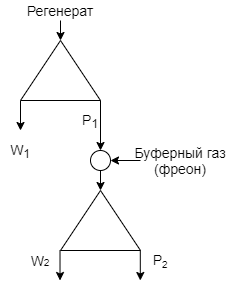
\includegraphics[scale=0.8]{cascades/p2_gas}}
  \caption{Каскад с газом-носителем}\label{p2_gas}
\end{figure}
 

Данная каскадная схема имеет схожие достоинства и недостатки с описанным выше вариантом двойного каскада. Характерным отличием схемы с газом-носителем является более высокая степень извлечения  $^{235}$U и более высокая степень очистки от $^{232}$U. С другой стороны, рассматриваемая схема схема имеет и характерные недостатки, которые заключаются в следующем:
\begin{enumerate}
  \item	отделение $^{232}$U от $^{235}$U за счет использования «газа-носителя» провоцирует рост концентрации $^{236}$U в получаемом товарном НОУ. Данное обстоятельство может иметь негативные последствие в условиях многократного рецикла урана в топливе реакторов на тепловых нейтронах. Это связано с тем, что рост концентрации $^{236}$U на каждом рецикле будет способствовать росту концентрации $^{232}$U \cite{smirnovEvolutionIsotopicComposition2012};
  \item	использование «газа-носителя» на разделительном производстве требует создания отдельной инфраструктуры по обращению с ним, а также отделению от него товарного гексафторида урана, что может сказаться на величине удельных затрат на получение товарного НОУ;
\end{enumerate}


Рассмотрим некоторые другие модификации двойных каскадов. В работе \cite{SposobIzotopnogoVosstanovleniyac} предложен вариант двойного каскада, состоящего из последовательно соединенных ординарного каскада и каскада с двумя внешними питаниями и дополнительным (промежуточным) потоком отбора (рис. \ref{fig:double_crazy}.

\begin{figure}[ht]
  \centerfloat{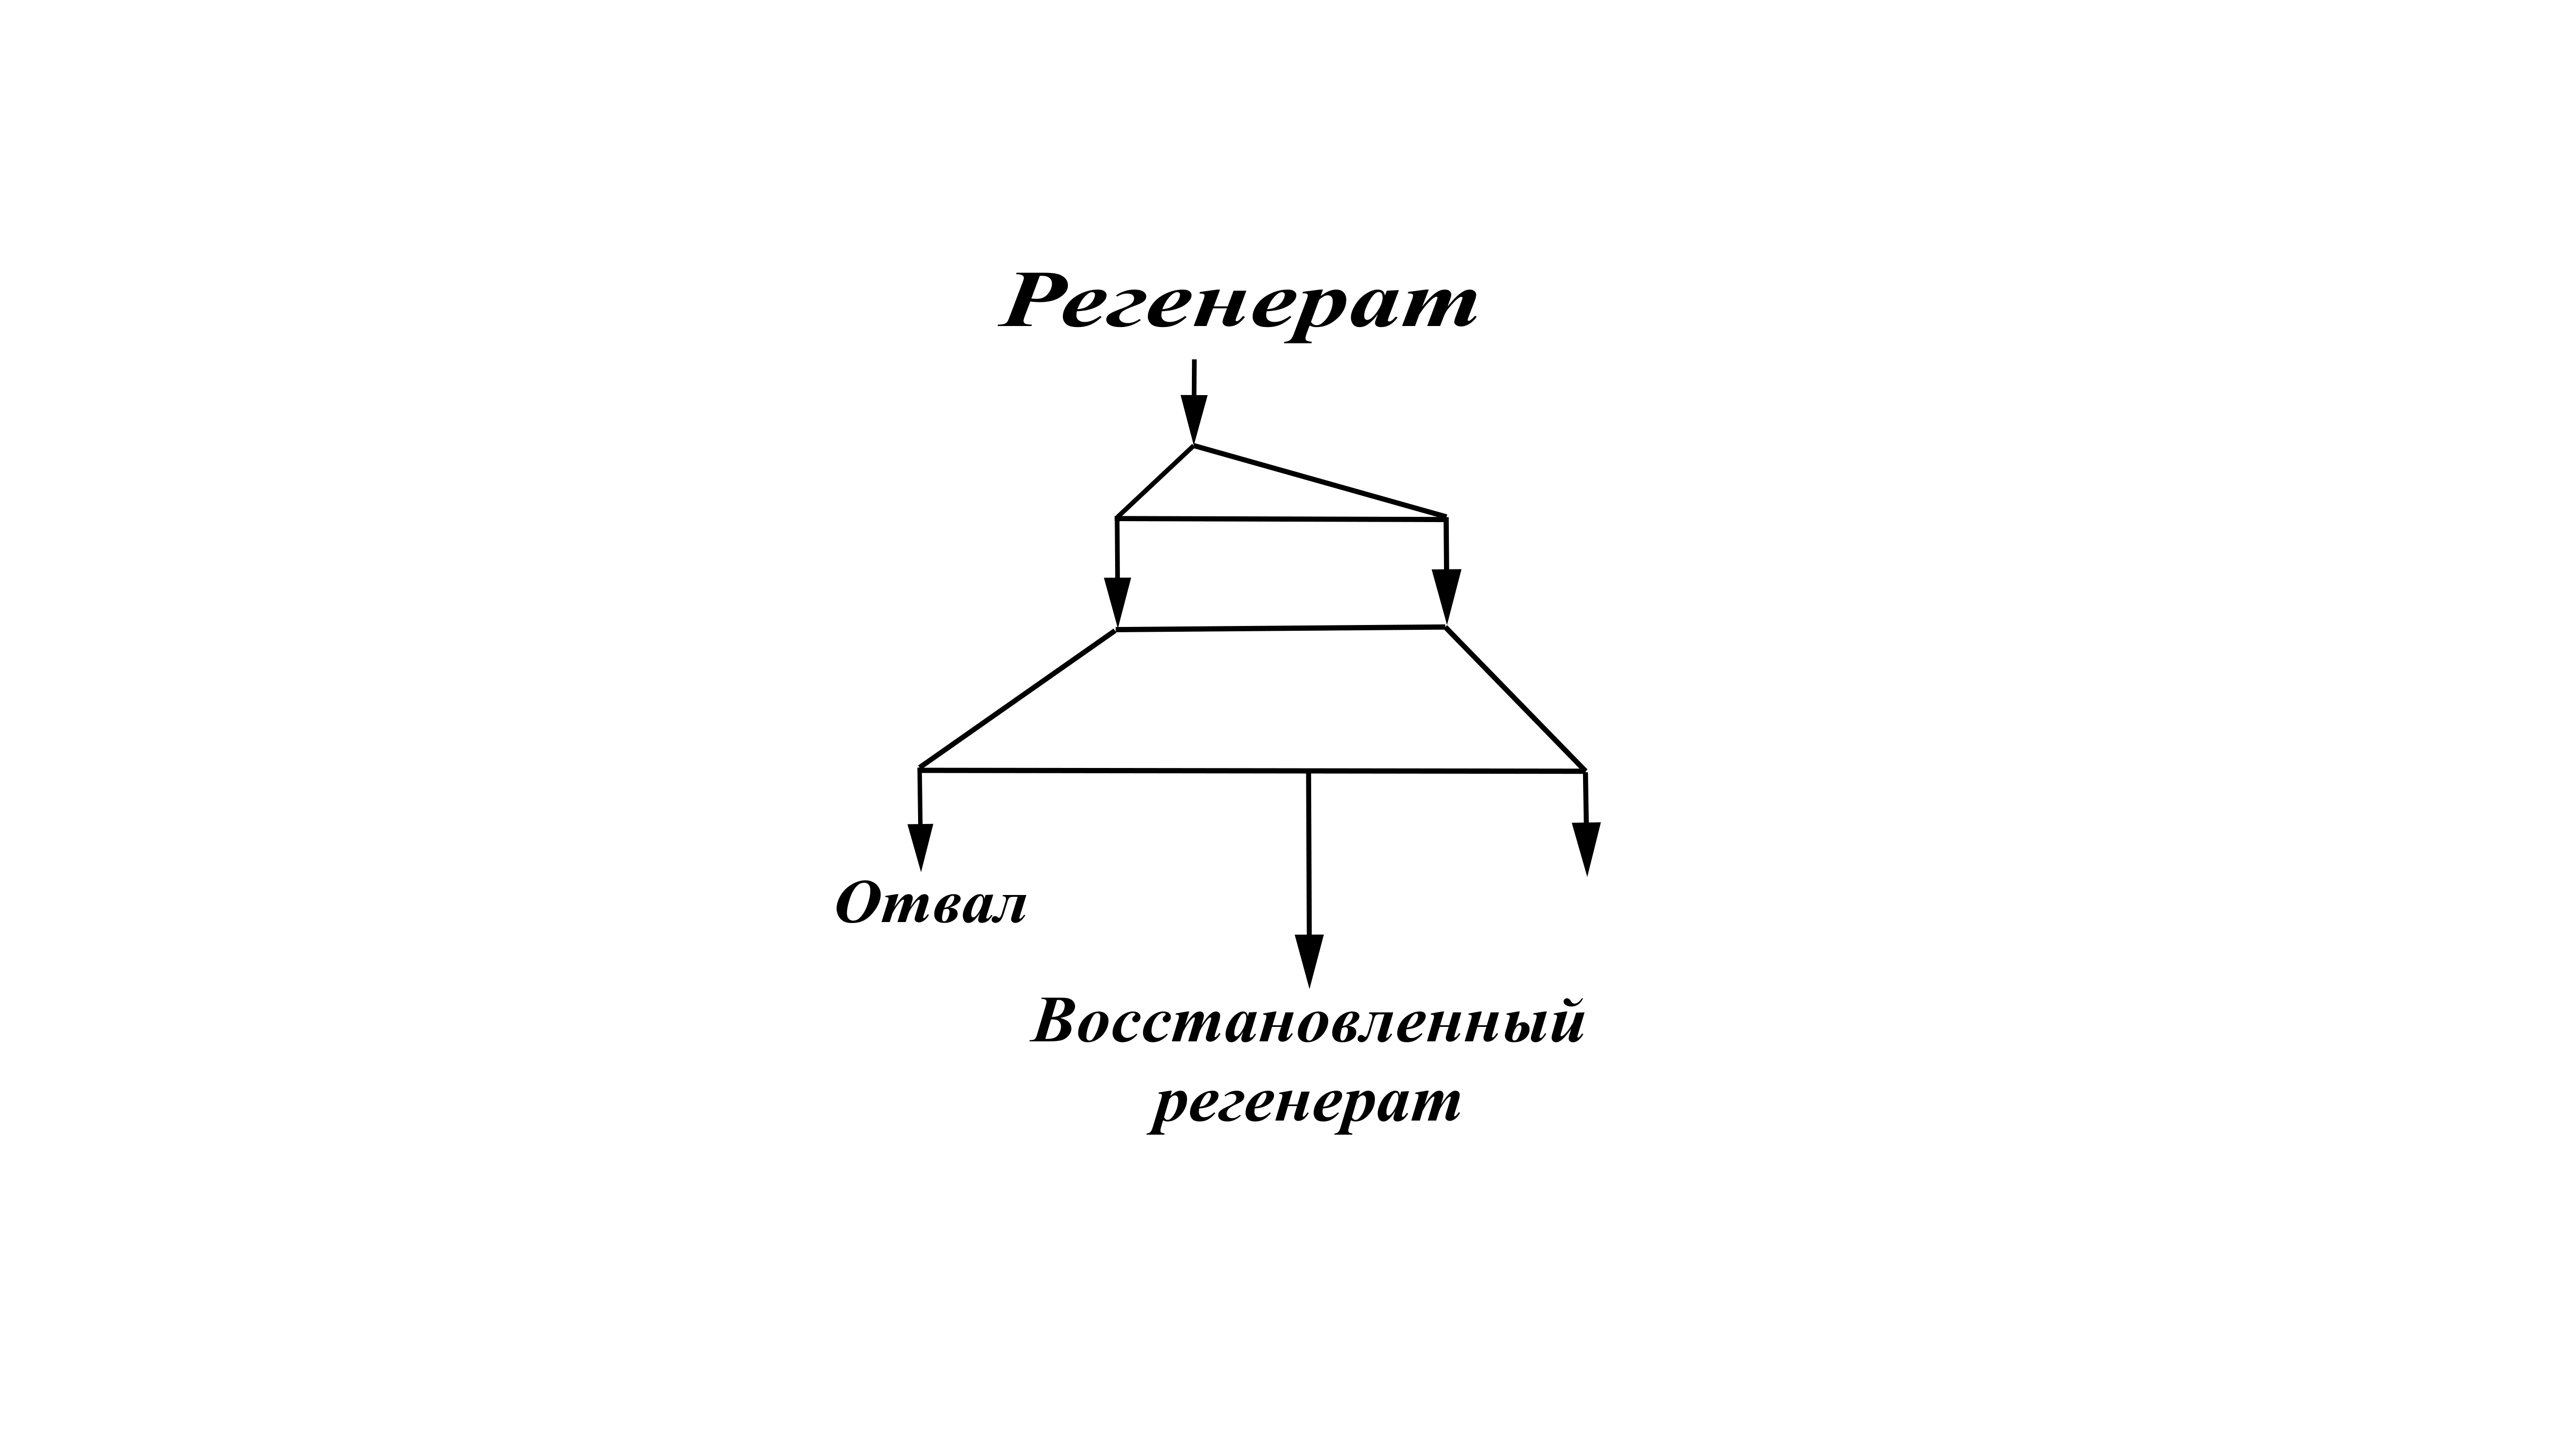
\includegraphics[scale=0.1]{cascades/double_crazy}}
  \caption{Двойной каскад на основе пятипоточного каскада, производящий восстановленный регенерат в промежуточном потоке отбора}\label{fig:double_crazy}
\end{figure}).

Как следует из рисунка \ref{fig:double_crazy} потоки отбора и отвала первого каскада поступают в качестве двух питаний второго каскада. Такая организация потоков между каскадами позволяет добиться разделения исходной смеси на группы, компоненты которых концентрируются в различных частях второго каскада. В итоге на внутренних ступенях оказывается сконцентрирован $^{235}$U, откуда его можно отобрать, использую включенный здесь дополнительный поток отбор. На концевых ступенях происходит отбор обедненного урана в потоке отвала второго каскада, а на другом конце каскада, в потоке лёгкой фракции получают поток, загрязненный изотопами $^{232}$U, $^{234}$U, который фактически является отходом рассматриваемой каскадной схемы. Тем не менее, в отличие от ранее рассмотренных вариантов двойного каскада в рассматриваемой схеме возможно избежать появления фракции, высокообогащенной по $^{235}$U, что важно с точки зрения вопросов обеспечения ядерного нераспространения. Однако, в соответствии с результатами \cite{SposobIzotopnogoVosstanovleniyac} поток легкой фракции второго каскада имеет обогащение по $^{235}$U на уровне 20,0\%, что означает потери изотопа $^{235}$U в этом потоке. При этом обогащение $^{235}$U в потоке отбора первого каскада составляет величины в диапазоне 5,0--10,0\%.
 
Таким образом, в данной схеме удается снизить потери работы разделения по сравнению с простейшими модификациями двойных каскадов. Однако остальные недостатки двойных каскадов присущи также и данной схеме. 

Завершая обзор наиболее характерных вариантов двойных каскадных схем, отметим следующее. 
Ключевым достоинством двойных каскадов является то, что они позволяют менять соотношения между концентрациями четных изотопов и $^{235}$U. Иными словами в них происходит очистка, а не разбавление регенерата. Это обстоятельство особенно важно при рассмотрение вопросов обогащения регенерата в условиях его многократного рецикла, когда концентрации чётных изотопов урана возрастают от рецикла к рециклу.
Однако двойные каскады имеют и ряд общих недостатков, среди которых можно выделить:

\begin{itemize}
  \item наличие отхода в виде фракции, загрязненной четными изотопами. Выработка стратегии по обращению с этой фракцией требует отдельных исследований. При этом наличие таких загрязненных фракций приводит к необходимости введения дополнительных мер радиационной безопасности на производстве. В результате практическая реализации подобных мер может изменить технологические подходы, принятые на разделительных производствах и, соответственно, повлиять на удельные затраты при производстве товарного НОУ; 
  \item	двойные каскады сами по себе принципиально не могут решить задачу «полного использования регенерата», поскольку принципиально производят продукта, в несколько раз меньше, чем требуется. Это обусловлено тем, что они не практически не используют других источников изотопа $^{235}$U, кроме регенерированного урана, содержания $^{235}$U в котором недостаточно для формирования новой загрузки реактора из ОЯТ которого он был выделен. Учитывая выше сказанное, с использованием двойных каскадов возможно обеспечить получение только части ТВС для новой загрузки реактора. Недостающая масса НОУ может быть получена, например, из природного урана путём его обогащения в ординарном каскаде.
\end{itemize}


\subsubsection{Гибридные схемы каскадов для обогащения регенерата урана}

Учитывая, что двойные каскады в общем случае не могут полностью решить сформулированную выше задачу обогащения регенерата, к настоящему моменту предложены способы обогащения регенерата урана, в которых сочетаются характерные особенности каскадных схем с разбавлением чётных изотопов и двойных каскадов. Ниже кратко проанализированы подобные способы.
Одним из вариантом таких гибридных схем является последовательное соединение одиночного каскада с двумя питаниями и ординарного каскада (рис.\ref{f_2double}) \cite{palkinOchistkaRegenerirovannogoGeksaftorida2013}. Подобную схему можно реализовать двумя способами, отличающимися тем, какой из выходящих потоков первого каскада подают на вход второго (рис. \ref{fig:2_inputs}).


\begin{figure}[ht]
  \centerfloat{\includegraphics[scale=0.5]{cascades/2double}}
  \caption{Варианты соединения двухкаскадной схемы, состоящей из каскада с двумя потоками питания и ординарного каскада: а) случай подачи отбора первого каскада на питание второго; б) случай подачи отвала второго каскада на питание второго каскада. Обозначения: $F_{nat}$ -- поток природного урана; $F_{rep}$ -- поток регенерата, направленного на обогащение; $P_1$ -- поток «легкой» фракции каскада 1; $W_1$ – поток «тяжелой» фракции каскада 1; $P_2$ -- поток «легкой» фракции каскада 2; $W_2$ -- поток «тяжелой» фракции каскада 2}\label{f_2double}
\end{figure}


В рассматриваемой схеме в первом каскаде получают НОУ промежуточного обогащения, меньшего, чем требуется для получения товарного НОУ. Затем, во втором каскаде данный промежуточный материал обогащают/обедняют в одном из выходящих потоков до уровня концентрации в исходном регенерированном уране, в зависимости от того из какого потока первого каскада был получен промежуточный материал. В результате с помощью схемы на выходных потоках второго каскада производится как обогащенный товарный продукт, так и урановая смесь с концентрацией $^{235}$U на уровне исходного регенерата, но с пониженным содержанием четных изотопов. Ключевым преимуществом данной схемы, в отличие от ранее рассмотренных двухкаскадных схем, является отсутствие на каких-либо ступенях каскада концентрации $^{235}$U, превышающей уровень низкообогащенного урана.
Тем не менее, по своей сути схема является, во многом, «разбавляющей», поскольку основной эффект очистки связан с наличием в первом каскаде дополнительного питания, в котором туда поступает природный уран, выступающий в качестве разбавителя. Как показал анализ результатов вычислительных экспериментов, проведенных для данной схемы в рамках настоящей работы (Приложение 1), данная каскадная схема позволяет решить задачу обогащения регенерата в сформулированной выше общей постановке только для случая  обогащения состава регенерата с относительно невысоким исходным содержанием чётных изотопов. Это означает, что данную каскадную схему затруднительно использовать для обогащения регенерата в условиях его многократного рецикла.

Ещё одним вариантом гибридной схемы обогащения регенерированного урана можно считать каскадную схемы, основанную на очистке регенерата от четных изотопов в одиночном каскаде, имеющем так называемое "расширение" потока \cite{palkinRestorationIsotopicComposition2020}. В этом подходе использован принцип выделения изотопов промежуточных массовых чисел из многокомпонентных смесей стабильных изотопов в каскадах с дополнительными потоками отбора \cite{smirnovQKASKADYDLYaPOLUChENIYa2013,smirnovVliyanieProfilyaPotoka2010,palkinMnogopotochnyeKaskadyDlya2015}. 
Основная идея работы подобной схемы состоит в том, что, подобрав соответствующим образом вид функции распределения потока питания по ступеням каскада, возможно добиться концентрирования целевого промежуточного компонента на внутренних ступенях. Организовав на ступени в области максимума концентрации целевого промежуточного компонента внутри каскада поток дополнительного отбора, возможно получить фракцию с максимальным содержанием этого изотопа при более низких по отношению к нему концентрациях легких изотопов, чем в отборе на конце каскада.
Описываемый эффект продемонстрирован как на примере модельного Q-каскада, так и на примере каскада постоянной ширины \cite{smirnovDesignCascadeLocally2015}. Каскады, имеющие подобную особенность в распределении потока питания по ступеням были названы каскадами с «расширением» потока \cite{smirnovVliyanieProfilyaPotoka2010}.

Учитывая, что изотоп $^{235}$U является промежуточным по массовому числу в смеси регенерированного урана этот способ можно применить и для концентрирования данного изотопа при обогащении регенерата урана. После чего, перемешав, полученный в промежуточном отборе такого каскада обогащенный регенерат, например, с обедненным ураном можно получить НОУ товарного качества.

Подобная каскадная схема схематично изображена на рисунке \ref{fig:enl}. Принцип работы данной схемы можно описать следующим образом. На вход каскада подают поток регенерированного урана $E_1$. Каскад имеет три выходящих потока: поток отвала $W_1$, поток дополнительного отбора G и поток основного отбора $P_1$. В потоке дополнительного отбора (G) достигается максимальное обогащение по $^{235}$U, которое составляет величину около 90\% или выше \cite{palkinRestorationIsotopicComposition2020}. В потоке отбора $P_1$ каскада нарабатывают смесь, высокообогащенную по $^{234}$U (до уровня 80\% и выше) и изотопу $^{232}$U (до уровня 3--10\%). Концентрация $^{235}$U в потоке $P_1$ лежит в диапазоне 10–-20\%. Материал, полученный в потоке G, далее необходимо перемешать с составом, имеющим низкое содержание $^{235}$U, для получения товарного продукта с одновременным снижением концентраций четных изотопов. В качестве разбавителя удобно использовать обедненный уран (поток DepU). После смешивания потоков $E_1$ и DepU получают состав урана, обладающий необходимой для товарного продукта концентрацией $^{235}$U и удовлетворяющий ограничениям на концентрации четных изотопов.
Процесс очистки в данной схеме состоит в отделении легкой группы изотопов ($^{232}$U и $^{234}$U) от целевого $^{235}$U при одновременном снижении относительной концентрации $^{235}$U и $^{236}$U. Фактически данная схема очищает регенерат в процессе его обогащения одновременно от всех четных изотопов. После чего происходит разбавление обедненным ураном фракции с высоким содержанием изотопа $^{235}$U, получаемой в потоке дополнительного отбора. В процессе такого разбавления происходит также и окончательная коррекция содержания чётных изотопов в получаемой смеси.
Как показали представленные в Приложении 1 расчёты, проведенные для подобной каскадной схемы, её эффективность и возможность решения поставленной задачи обогащения регенерированного урана существенно зависят от состава исходной разделяемой смеси. Данный фактор затрудняет её использование в условиях многократного рецикла урана. 

\begin{figure}[ht]
  \centerfloat{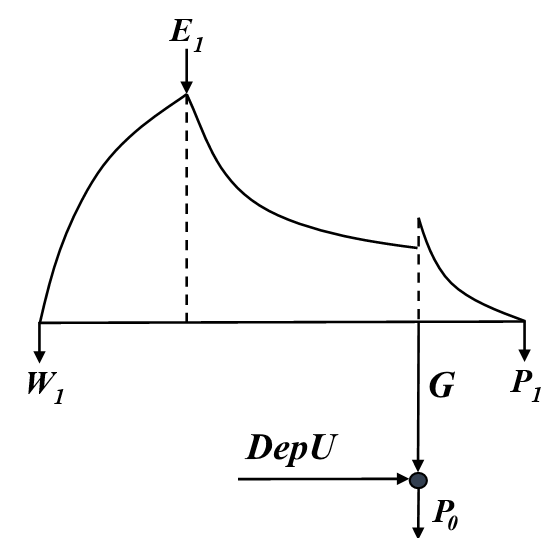
\includegraphics[scale=0.5]{cascades/enl}}
  \caption{Схема каскада концентрирования $^{235}$U в дополнительном отборе и последующим разбавлением обедненного урана для получения товарного НОУ. Обозначения: $E_1$ –- поток регенерата, направленного на обогащение; $P_1$ –- поток «легкой» фракции; $W_1$ –- поток отвала; G –- поток дополнительного отбора; DepU –- поток обедненного урана; $P_0$ –- поток товарного НОУ.
  }\label{fig:enl}
\end{figure}


К достоинствам схемы можно отнести следующее:

\begin{enumerate}
  \item полное отсутствие природного урана в схеме;
  \item эффект коррекции изотопного состава достигается не только за счет разбавления, но и за счет снижения относительных концентрации четных изотопов к $^{235}$U (в первую очередь, $^{236}$U) в самом каскаде.
\end{enumerate}

К недостаткам схемы можно отнести следующее:
\begin{enumerate}
  \item высокие уровни активности на разделительном производстве ввиду наличия потоков с концентрациями четных изотопов на порядки, превышающими допустимые пределы для низкообогащенного урана и уранового сырья. Возможность работы разделительного производства при уровне концентрации $^{232}$U свыше 10--3\% и с фракцией, содержащей практически «чистый» $^{234}$U требует отдельной проработки с точки зрения вопросов радиационной безопасности и проблемы радиолиза рабочего вещества; 
  \item данная схема в общем случае не позволяет обеспечить условие «полного использования регенерата».
\end{enumerate}


\section{Выводы из анализа предложенных способов обогащения регенерированного урана}

Подводя итог раздела, известные на сегодняшний день технические решения задачи обогащения регенерированного урана с одновременной коррекцией его изотопного состава основаны на:
\begin{enumerate}
  \item разбавлении регенерированного урана материалами, не содержащими четных изотопов (например, природным ураном, обедненным ураном и т.д.), на входе в разделительный каскад, на выходе из разделительного каскада или внутри каскада при подаче разбавителей в качестве дополнительных внешних питаний каскада;
  \item использовании каскадных схем, позволяющих понижать относительные концентрации чётных изотопов по отношению к $^{235}$U (преимущественно двойные каскады и их модификации);
  \item комбинировании процессов разбавления регенерата материалами, не содержащими чётных изотопов, и его очистки за счёт выведения нежелательных фракций с относительно высоким содержанием $^{232}$U и $^{234}$U в виде отдельных потоков.
\end{enumerate}

Проведенный теоретический анализ наиболее характерных каскадных схем каждого из типов позволяет сделать следующие выводы:
\begin{enumerate}
  \item наиболее перспективные варианты решения задачи обогащения регенерата в условиях многократного рецикла могут быть основаны на использовании модификаций «гибридных» каскадных схем, поскольку они одновременно позволяют корректировать как изотопный состав регенерата за счёт его частичной очистки от чётных изотопов, так и массовые расходы за счёт варьрования величин потоков разбавителей;
  \item проведенная серия вычислительных экспериментов с целью оценки возможности обогащения регенерированного урана, прошедшего несколько рециклов, показала, что ни одна из описанных выше схем не может быть применена для решения задача обогащения регенерата в условиях многократного рецикла в наиболее общей постановке;
  \item актуальным становится поиск каскадной схемы, позволяющей решить в общем случае задачу обогащения регенерата при различном исходном содержании регенерата в нём.
\end{enumerate}           % Глава 1
\chapter{Анализ физических ограничений для решения задачи в ординарных и двойных каскадах}\label{ch:ch2}

Как уже было отмечено в главе 1, лишь некоторые из предложенных к настоящему моменту способов обогащения регенерированного урана потенциально способны решить задачу обогащения регенерата произвольного исходного состава в условиях одновременного выполнения ограничений на концентрации сразу нескольких изотопов и при заданной пропорции между продуктом и исходной смесью. В первую очередь, это касается разбавляющих схем на основе ординарного каскада. 
Однако проведенный ранее теоретический анализ не позволяет однозначно утверждать при каких условиях может быть применена та или иная схема. В рамках настоящей главы кратко представлены результаты серии вычислительных экспериментов и сопутствующего им теоретического анализа, направленных на то, чтобы выявить область возможного применения одиночных каскадных схем с разбавлением и двойных каскадов для получения обогащенного регенерированного урана в условиях многократного рецикла. 

\section{Постановка задачи и методическая часть}

Для изучения возможностей разбавляющих схем на основе ординарного каскада были рассмотрены случаи обогащения регенерированного урана с различным исходным содержанием чётных изотопов, где изотопные составы с номерами 1 и 2 соответствуют регенерату второго и пятого рецикла, соответственно (см. таблицу \ref{is_compositions_2_5}). Выбранные составы отвечают регенерированному урану, выделенному из ОЯТ реакторов ВВЭР-1000 и -1200 при различных внешних условиях \cite{palkinDesignanalyticalResearchRefinement2010,nevinicaToplivnyyCiklLegkovodnogo2019}. Отметим, что оба состава характеризуются довольно высоким содержанием $^{232}$U. Выбор подобных загрязненных четными изотопами составов регенерата имитирует сложности, которые могут возникать при обогащении регенерированного урана в условиях многократного рецикла.  
При реализации вычислительных экспериментов общая постановка задачи соответствовала формулировке, приведенной в Главе 1. С учётом конкретных выбранных ограничений задачу можно сформулировать следующим образом.

Из заданной массы исходного регенерированного урана необходимо получить заданную массу товарного НОУ, отвечающего следующим требованиям:

\begin{enumerate}
  \item Концентрация в конечном продукте составляет 4,95\%, значение характерно для современных легководных реакторов \cite{solovevaCennostiOYaTKak2019}.
  \item Расход регенерированного урана на единицу конечного продукта в виде низкообогащенного урана: 0,93 кг на 1 кг НОУ \cite{smirnovApplyingEnrichmentCapacities2018}.
  \item Концентрация $^{235}$U в потоке отвала задана равной 0,1\% \cite{smirnovEvolutionIsotopicComposition2012};
  \item Соотношение $^{234}$U к $^{235}$U не должно превышать 0,02.
  \item Влияние изотопа $^{236}$U на нейтронно-физические характеристики топлива должно быть скомпенсировано дополнительным обогащение по $^{235}$U, для расчёта которого коэффициент компенсации реактивности принят равным 0,29 \cite{smirnovApplyingEnrichmentCapacities2018}.
  \item Концентрация $^{232}$U ограничена величиной $5\cdot10^{-7}$\% \cite{smirnovApplyingEnrichmentCapacities2018}.
\end{enumerate}

В качестве схем обогащения регенерированного урана рассмотрены схемы, представленные на рисунке \ref{fig:diagram1}.
Каждая из них подразумевает использование ординарного каскада. Для моделирования процессов обогащения урана в каскаде использовали модель R-каскада \cite{sulaberidzeTeoriyaKaskadovDlya2011}. При этом во всех случаях при расчёте параметров каскада задавали концентрации $^{235}$U в его внешних выходящих потоках. Под расчётом параметров такого каскада подразумевали следующую задачу. 
Задано: состав обогащаемой смеси; параметры одиночного разделительного аппарата; величина одного из внешних потоков каскада, например, потока отбора или питания; концентрации $^{235}$U в потоках отбора и отвала каскада; в случае расчёта на основе модели R-каскада задают также пару компонентов, по относительным концентрациям которых выполняется условие несмешивания.
В процессе расчёта необходимо определить следующие параметры: число ступеней в каскаде и номер ступени подачи внешнего питания, концентрации всех компонентов (кроме $^{235}$U) в выходящих из каскада потоках, величины неизвестных внешних потоков каскада, распределения потока и концентраций компонентов по ступеням каскада и все остальные внутренние параметры. 
Такая постановка задачи требует численного решения системы нелинейных уравнений, возникающих для невязок концентраций $^{235}$U в выходящих потоках. Указанная система может быть записана в следующем виде: 

$\Delta_{P} = {(C_{235, P})}_{calc}-{(C_{235, P})}_{given}$

$\Delta_{W} = {(C_{235, W})}_{calc}-{(C_{235, W})}_{given}$

где ${(C_{235, P})}_{calc}$, ${(C_{235, W})}_{calc}$ - рассчитанные концентрации $^{235}$U в потоках отбора и отвала каскада, соответственно; ${(C_{235, P})}_{given}$, ${(C_{235, W})}_{given}$ - заданные концентрации $^{235}$U в потоках отбора и отвала каскада, соответственно; $\Delta_{P}$, $\Delta_{W}$ -- невязки по концентрациям $^{235}$U в потоках отбора и отвала каскада, соответственно. 

Для получения уравнений на невязки использованы соотношения (\ref{GrindEQ__1_72_}), (\ref{GrindEQ__1_73_}). Из решения подобной системы можно определить величины $R_{n k}^{W}$ и $R_{n k}^{P}$, после чего аналитически рассчитать остальные внешние параметры R-каскада по соотношениям (\ref{GrindEQ__1_70_})-(\ref{GrindEQ__1_77_}).   


\begin{table}[h]
  \centering
  \normalsize\begin{tabulary}{1.0\textwidth}{|c|c|c|c|c|c|c|}
  \hline Состав № & Массовое число & 232 & 233 & 234 & 235 & 236 \\
  \hline 1 & C, \% & $6,62\cdot10^{-7}$ & $1,19\cdot10^{-6}$ & $3,28\cdot10^{-2}$ & 1,43 & 0,9932 \\
  2 & C, \% &  $1,03\cdot10^{-6}$ & $1,3\cdot10^{-6}$ & $3,91\cdot10^{-2}$ & 1,07 & 1,45 \\\hline
  \end{tabulary}
  \caption{{Изотопные составы регенерата различных циклов.{\label{is_compositions_2_5}}}}
\end{table}

Ниже представлены результаты моделирования обогащения регенерата в каждой из трёх схем, представленных на рисунке \ref{fig:diagram1}. 
Основная цель проведенного моделирования - оценить возможность использования схем на основе ординарного каскада для обогащения регенерированного урана с повышенным содержанием чётных изотопов и, в первую очередь, $^{232}$U. Во всех случаях в качестве обогащаемого состава был рассмотрен состав, соответствующий второму рециклу и, как следствие, имеющий более низкое содержание чётных изотопов, по отношению к составу пятого рецикла.

\subsection{Схема с разбавлением предварительно обогащенного регенерата}

Рассмотрим каскадную схему, в которой регенерат сначала обогащают до уровня, превышающего необходимую концентрацию $^{235}$U, а затем разбавляют, например, природным ураном (рис. \ref{o1}). Такая схема позволяет обогатить регенерат до требуемого условием задачи содержания изотопа $^{235}$U в конечном продукте (НОУ), а также выполнить ограничения на $^{232}$U и другие изотопы. При этом необходимо проверить соблюдение и остальных условий решаемой задачи обогащения регенерата. Заметим, что данная схема также подразумевает возможность использования в качестве разбавителя любой другой урановой смеси, не содержащей изотопов $^{232}$U и $^{236}$U. В качестве одного из вариантов разбавителей может быть использован и низкообогащенный уран, полученный обогащением природного урана.

\begin{figure}[ht]
  \centerfloat{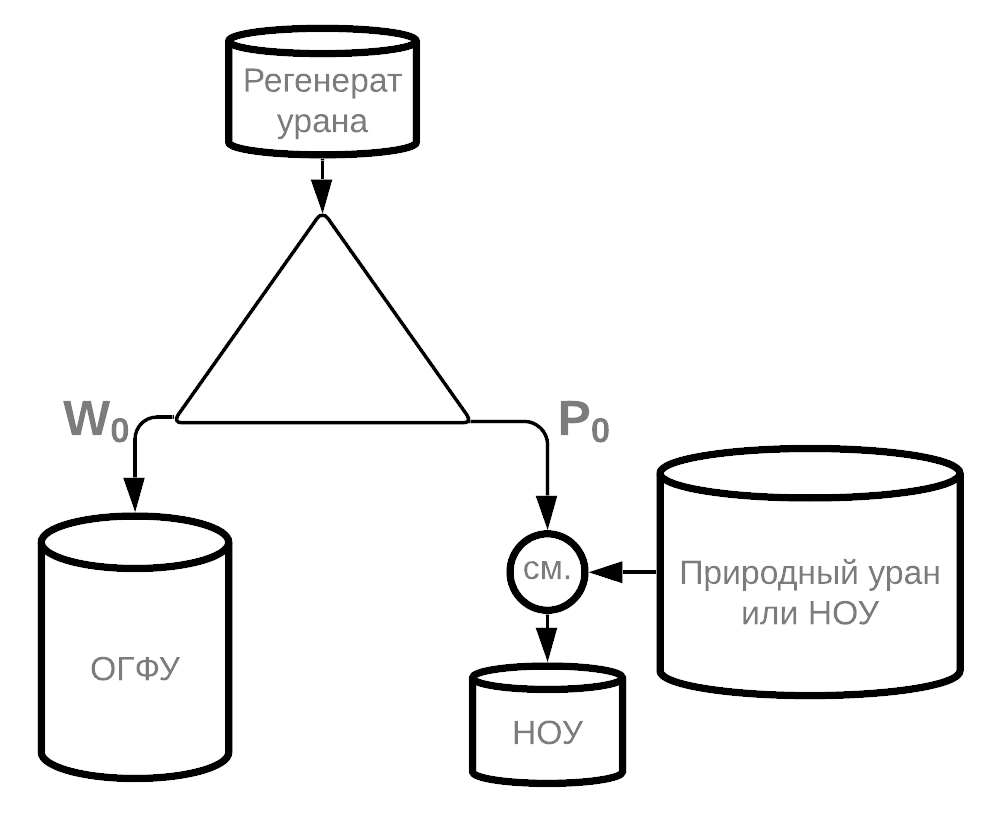
\includegraphics[scale=0.2]{cascades/ordinary/1}}
  \caption{Схема разбавления предварительно обогащенного регенерата природным ураном или низкообогащенным ураном. Обозначения: $P_0$ -- поток отбора легкой фракции каскада; $W_0$ -- поток отвального ОГФУ тяжелого конца каскада; $CM.$ -- узел смешения, на выходе из которого получается конечный продукт $НОУ$ -- низкообогащенный уран}\label{o1}
\end{figure}

Для получения обогащенного урана, удовлетворяющего всем требованиям, необходимо определить величину концентрации $^{235}$U в потоке $P_0$ и пропорцию смешивания потоков $P_0$ и разбавителя. Указанные параметры определяли итерационно по следующей схеме. Сначала задавали начальное приближение для концентрации $^{235}$U в потоке $P_0$, после чего рассчитывали параметры каскада по описанной в предыдущем разделе процедуре. Далее, зная состав смеси урана в потоке $P_0$ на основе простейшей пропорции определяли соотношение между потоками природного урана или обогащенного регенерата для получения финального продукта. При этом полученный в результате смешивания поток товарного НОУ должен отвечать ограничениям по концентрациям чётных изотопов, а отношение массы полученного НОУ к массе исходного регенерата должно соответствовать заданной величине. Это означает, что для успешного решения задачи одновременно должны быть выполнены условия на концентрации изотопов $^{232,234,235,236}$U и обеспечена заданная пропорция между расходом регенерата и конечным продуктом. Однако при известной и заданной концентрации $^{235}$U в потоке разбавителя управляющих параметров в такой схеме только два: концентрация $^{235}$U в потоке $P_0$ и пропорция смешивания обогащенного регенерата и разбавителя. Очевидно, что в этом случае не для любых исходных данных возможно подобрать требуемые параметры каскадной схемы. 
Для иллюстрации сложности решения подобной задачи рассмотрим некоторые вспомогательные функции $\delta_1$ и $\delta_2$, которые определены следующим образом:

\begin{equation} \label{d1} 
  \delta_1=\left[C_{235}^P-\left(C_n^P+KKP\times C_{236}^P\right)\right]
\end{equation} 

\begin{equation} \label{d2} 
    \delta_2=\left[C_{232}^P-{(C_{232}^P)}_{lim}\right],             
\end{equation}

где ККР -- коэффициент компенсации реактивности, $(C_{232,P})_{lim}$ -- величина предельно допустимой концентрации $^{232}$U в товарном НОУ (например, $5\cdot10^{-7}$\%).

По своему физическому смыслу величина $\delta_1$ представляет собой отклонение концентрации изотопа $^{235}$U (выраженное в долях) в конечном продукте (после смешивания) от заданной величины, с учетом компенсации $^{236}$U. Величина $\delta_2$ представляет собой разность фактической концентрации $^{232}$U в окончательном продукте и требуемой величины в соответствии с принятым ограничением. Из таких определений очевидно, что в случае получения продукта, отвечающего необходимым условиям обе функции должны быть равны 0, причём при одних и тех же параметрах схемы. Фактически, функции $\delta_1$ и $\delta_2$ задают для рассматриваемой каскадной схемы систему уравнений, из которой можно найти её параметры при заданном отношении потоков регенерата и продукта. Оговоримся, что строго говоря к этой системе надо добавить аналогичное условие на концентрацию $^{234}$U, однако как будет показано ниже, даже в таком более простом варианте каскадная схема не может обеспечить одновременное выполнение всех требований, предъявляемых к составу конечного продукта.   

В рамках работы были проведены вычислительные эксперименты, в которых варьировали концентрацию $^{235}$U в потоке $P_0$, а пропорцию между $P_0$ и разбавителем из природного урана варьировали в диапазоне от 1 до 20. Для каждого случая пытались решить задачу обогащения регенерированного урана при описанных в разделе 3.1 внешних условиях задачи. Концентрацию $^{235}$U в потоке $W_0$ задавали равной 0,1\%. При расчёте параметров ординарного каскада во всех случаях предполагали, что в каскаде было реализовано несмешивание по относительной концентрации компонентов $^{235}UF_6$ и $^{236}UF_6$. Такое условие было выбрано на основе серии предварительных расчётов. Величину коэффициента разделения для компонентов  $^{235}UF_6$ к $^{238}UF_6$ приняли равной 1.2  \cite{smirnovEvolutionIsotopicComposition2012}. Все расчёты выполнены на примере регенерированного урана состава 1 таблицы \ref{is_compositions_2_5}.
На рис. \ref{delta1}--\ref{delta4} представлены зависимости величин $\delta_1$ и $\delta_2$ от соотношения смешиваемых потоков, взятых для различных значений концентрации $^{235}$U (рис. \ref{delta1}--\ref{delta4}) в потоке $P_0$. Чтобы сопоставить указанные величины на одном рисунке, величина $\delta_2$ была взята с поправкой (умножена на специально подобранный числовой коэффициент, который был равен $10^{-5}$).
Как видно из рисунков \ref{delta1}-\ref{delta4} функции $\delta_1$ и $\delta_2$ имеют <<нули>> при различных значениях аргумента. Таким образом, полученные результаты показывают невозможность одновременного удовлетворения условия компенсации $^{236}$U и выполнения заданного ограничения по $^{232}$U в получаемом товарном НОУ. По крайней мере это справедливо для рассмотренного изотопного состава. Дополнительные расчёты для состава пятого рецикла подтвердили те же выводы. Следовательно, данную схему нельзя рассматривать в качестве способа обогащения регенерированного урана в условиях его многократного рецикла.


\begin{figure}[ht]
  \begin{minipage}{.5\textwidth}
    \centering
    % include first image
    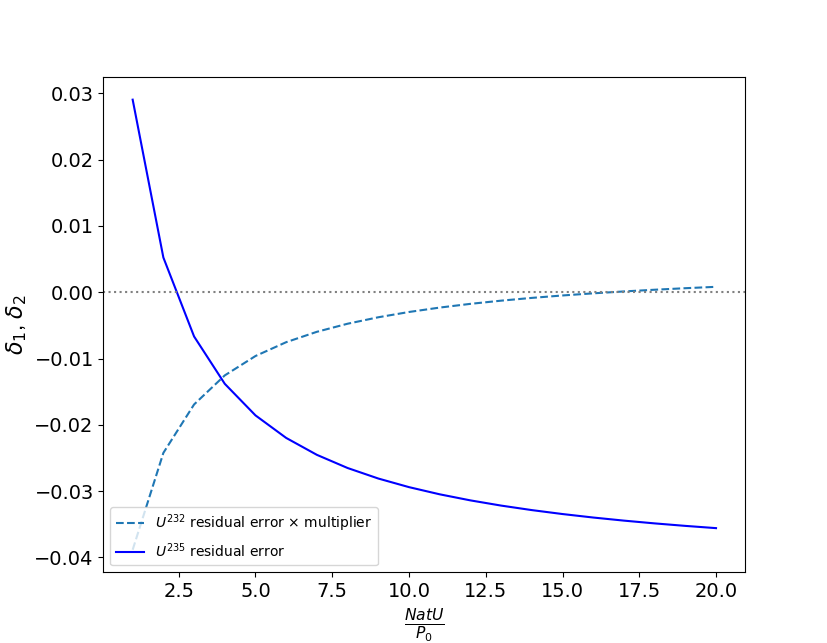
\includegraphics[width=.8\linewidth]{images/plots/15}  
    \caption{Концентрация $^{235}$U в предварительно обогащенном регенерата равна 15\%}
    \label{delta1}
  \end{minipage}
  \begin{minipage}{.5\textwidth}
    \centering
    % include second image
    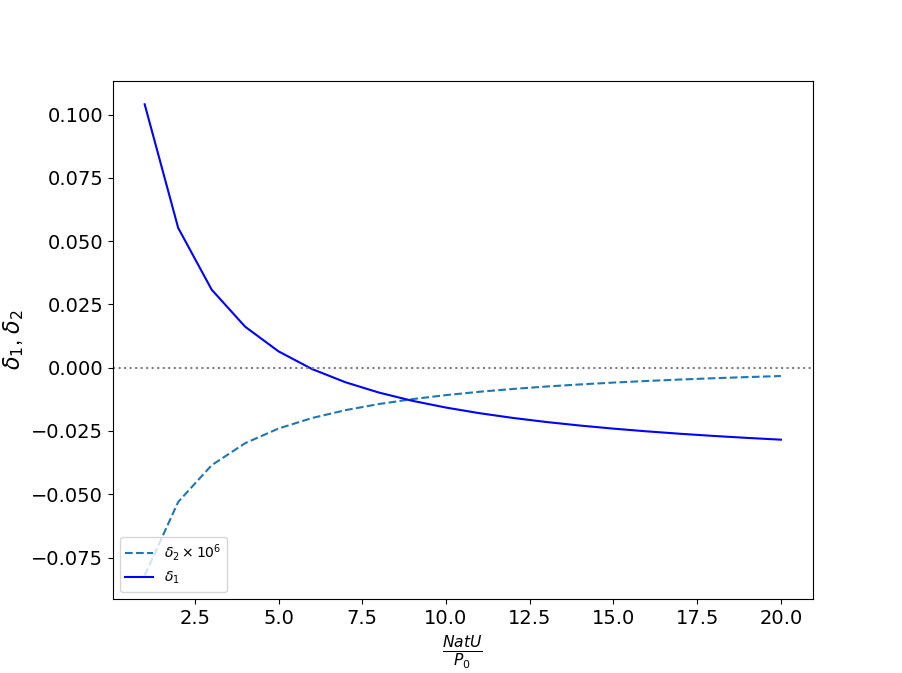
\includegraphics[width=.8\linewidth]{images/plots/30}  
    \caption{Концентрация $^{235}$U в предварительно обогащенном регенерата равна 30\%}
    \label{delta2}
  \end{minipage}
  \begin{minipage}{.5\textwidth}
    \centering
    % include second image
    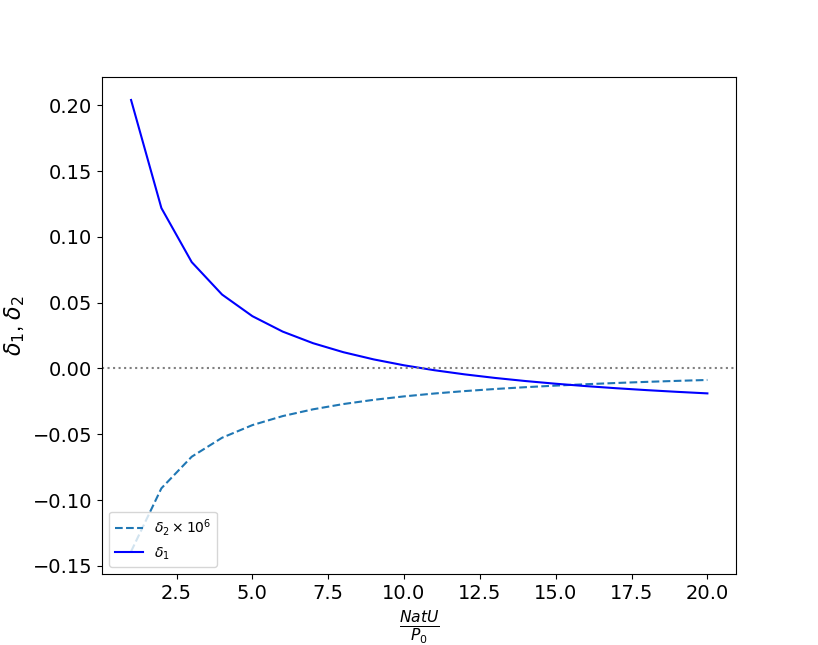
\includegraphics[width=.8\linewidth]{images/plots/50}  
    \caption{Концентрация $^{235}$U в предварительно обогащенном регенерата равна 50\%}
    \label{delta3}
  \end{minipage}
  \begin{minipage}{.5\textwidth}
    \centering
    % include second image
    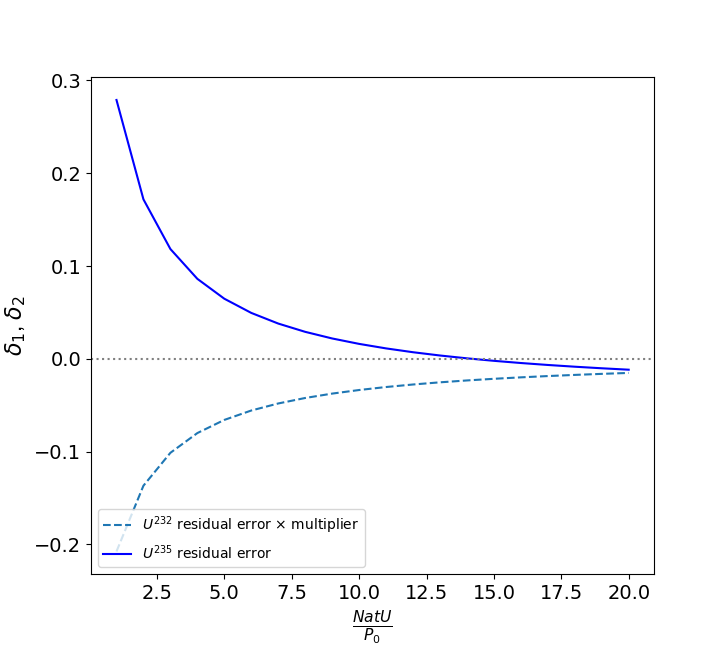
\includegraphics[width=.8\linewidth]{images/plots/65}  
    \caption{Концентрация $^{235}$U в предварительно обогащенном регенерата равна 65\%}
    \label{delta4}
  \end{minipage}
  % \caption{Невязки для $^{235}$U и $^{232}$U. Обозначения: $\frac{NatU}{P_{0}}$ -- отношение доли природного урана к потоку обогащенного регенерата.}
  % \label{fig:deltas_ordinar}
 \end{figure}


\subsection{Схема с разбавлением предварительно обогащенного регенерата низкообогащенным ураном}

Если в схеме, рассмотренной выше (рис. \ref{o1}), заменить разбавитель предварительно обогащенного регенерата (рис. \ref{o1}) с природного урана на низкообогащенный уран, не содержащий четных изотопов (например, изготовленный из природного урана), для данного состава можно найти решение, когда одновременно выполнены условия равенства нулю обеих невязок ($\delta_1$ и $\delta_2$). Данная схема может быть рассмотрена в качестве модификации варианта, описанного в предыдущем разделе. Нахождение решения для такой схемы обусловлено появлением дополнительного управляющего параметра -- концентрации $^{235}$U в потоке $НОУ$-разбавителя.  Несмотря на это, в подобном варианте каскадной схемы может быть не выполнено условие максимального использования регенерированного урана, состояющее в равенстве отношения потоков исходного регенерата и товарного НОУ заданной величине.

Чтобы оценить возможность решения задачи в рассматриваемой каскадной схеме проведены вычислительные эксперименты, в рамках которых варьировали следующие параметры схемы: концентрации $^{235}$U в потоках $P_0$ и $W_0$ (рис. \ref{o1}). Варьирование именно этих параметров позволяет менять относительные концентрации компонентов смеси, в том числе, и для пары изотопов $^{232}$U и $^{235}$U, тем самым обеспечивая получение различных вариантов изотопного состава конечного продукта. Для каждой комбинации варьируемых параметров пытались найти решение, удовлетворяющее внешним условиям, описанным в разделе 3.1. В качестве состава обогащаемого регенерата рассмотрен состав 1 таблицы \ref{is_compositions_2_5}.  

\begin{figure}[ht]
  \centerfloat{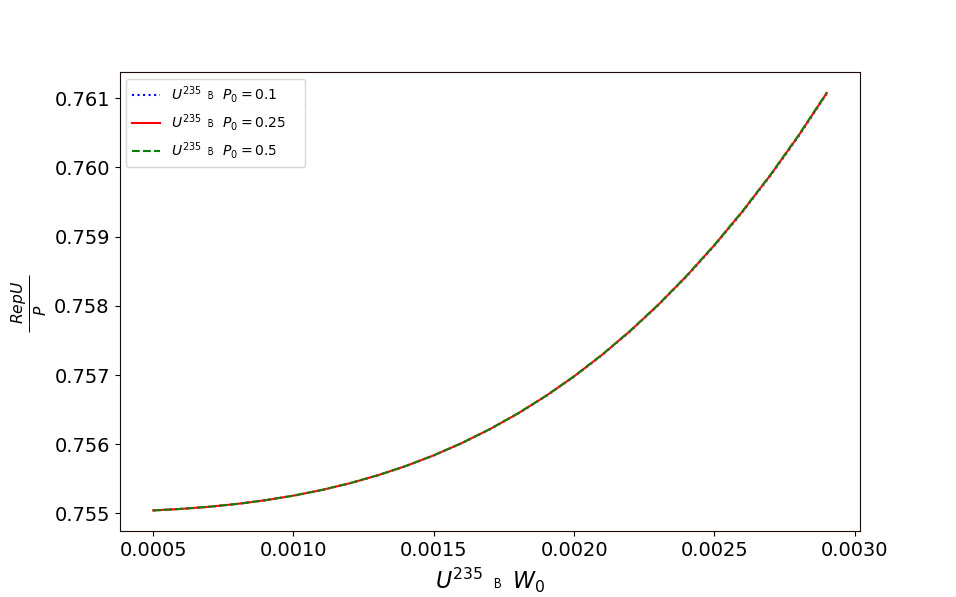
\includegraphics[scale=0.5]{images/plots/Figure_10ru}}
  \caption{Расход регенерата на единицу конечного НОУ-продукта для различных концентраций $^{235}$U в потоках продукта и отвала каскада, обогащающего регенерат}\label{Figure_10}
\end{figure}

\begin{figure}[ht]
  \centerfloat{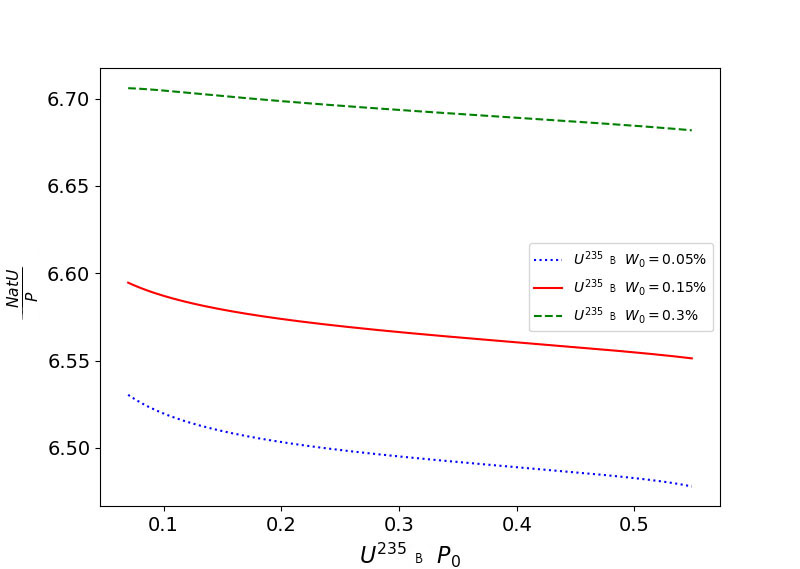
\includegraphics[scale=0.5]{images/plots/sc2_2ru}}
  \caption{Расход природного урана на единицу НОУ-продукта  для различных концентраций $^{235}$U в потоках продукта и отвала каскада, обогащающего регенерат}\label{fig:sc2_2}
\end{figure}

На рис. \ref{Figure_10}-\ref{fig:sc2_2} представлены зависимости отношения потоков исходного регенерата и конечного продукта, удельного расхода природного урана и потерь работы разделения при обогащении регенерированного урана в рассматриваемой каскадной схеме. 
Анализ кривых рисунка \ref{Figure_10}, отражающих зависимости расхода регенерата на единицу НОУ-продукта ($\frac{NatU}{P_{0}}$) от концентрации $^{235}$U в $W_0$ при трёх различных концентрациях данного изотопа в потоке $P_0$, показывает невозможность выполнить условия возврата заданной доли регенерата на единицу продукта в такой каскадной схеме ($^{235}$U в $W_0$ и в $P_0$) и при таком диапазоне варьирования её свободных параметров. Причем пропорция используемого регенерата к НОУ-продукту меняется лишь незначительно с изменением концентрации $^{235}$U в $W_0$. Тот факт, что кривые для рассмотренных значений концентрации $^{235}$U в $P_0$ фактически совпали означает, что изменение данного параметра может оказывать влияние на величину затрат работы разделения или расхода природного урана (см. рисунки \ref{fig:sc2_2}, \ref{Figure_13}), но не долю возвращаемого в воспроизводство топлива регенерата.
Как следует из анализа рисунка \ref{fig:sc2_2}, варьирование концентраций $^{235}$U в потоках $P_0$ и $W_0$ позволяет варьировать экономию природного урана, обсепечив величину удельного расхода на уровне $\approx$6,5-6,7 для всего исследуемого диапазона параметров. Это означает, что при заданном интервале параметров, рассматриваемая схема обеспечивает экономию природного урана на уровне 15--28\%, по сравнению со случаем получения НОУ только из природного сырья, для которого удельный расход природного урана составляет $\approx$7,93 (см. Приложение).

В качестве дополнительной иллюстрации полученных данных на рис.\ref{Figure_13} представлены зависимости относительных потерь работы разделения от величины концентрации $^{235}$U в потоке $W_0$ при различных концентрациях данного изотопов в потоке $P_0$. Область отрицательных значений потерь работы разделения на рис. \ref{Figure_13} соответствует ее экономии. Как следует из изучения характера кривых, уменьшение концентрации $^{235}$U в обедняемом потоке регенерата $W_0$ дает существенный вклад в экономию работы разделения, по-видимому, за счет более эффективного извлечения $^{235}$U из регенерата. Слияние кривых, соответствующих различным концентрациям $^{235}$U в обогащенном регенерате, обусловлено эквивалентностью масс $^{235}$U в каждом из этих потоков, что отражает постоянство вклада обогащенного регенерата в формирование конечного продукта.

% \begin{figure}[ht]
%   \centerfloat{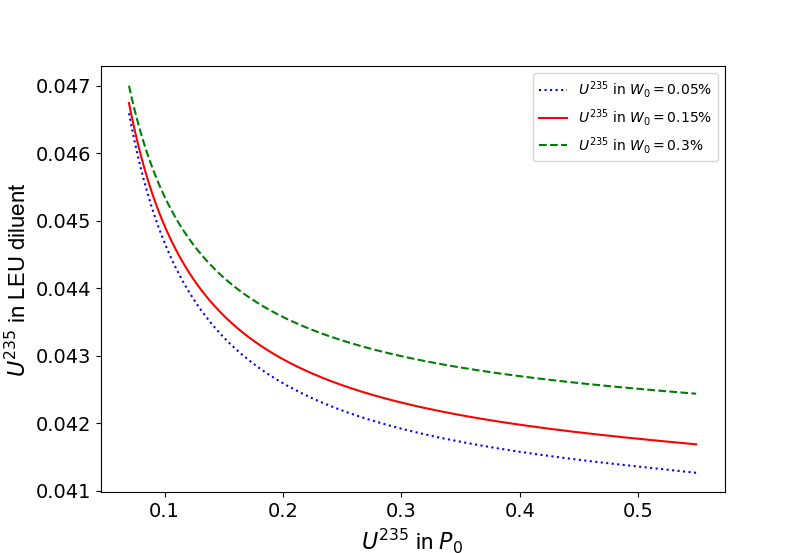
\includegraphics[scale=0.5]{images/plots/sc2_LEU_D}}
%   \caption{Концентрация $^{235}$U в разбавителе, необходимая для получения свежего НОУ для различных концентраций $^{235}$U в потоках продукта и отвала каскада, обогащающего регенерат}\label{fig:sc2_LEU_D}
% \end{figure}


\begin{figure}[ht]
  \centerfloat{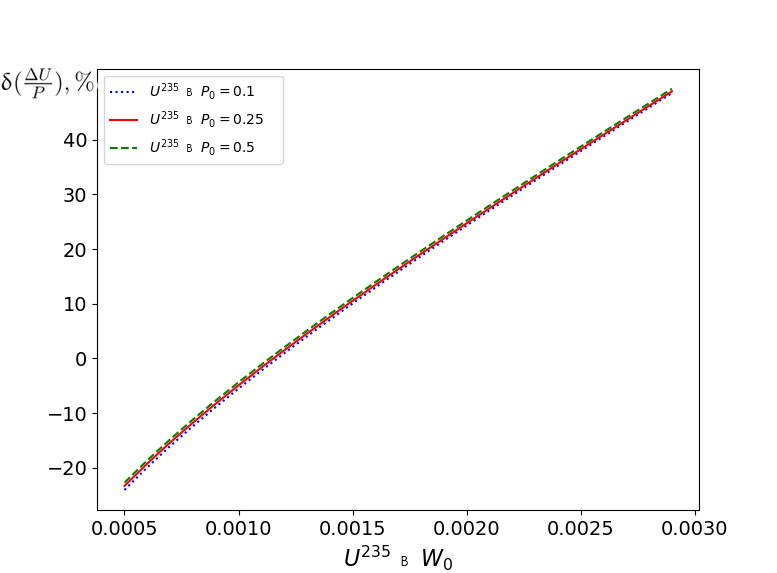
\includegraphics[scale=0.5]{images/plots/Figure_13ru}}
  \caption{Потери работы разделения по отношению к ординарному каскаду для обогащения природного урана для различных концентраций $^{235}$U в потоках продукта и отвала каскада, обогащающего регенерат}\label{Figure_13}
\end{figure}

% Проиллюстрировать затраты на работу разделения от составных  частей каскадной схемы, можно с помощью рис.\ref{myplot}, который показывает, что доля центрифуг для приготовления разбавителя из природного урана выше, чем доля центрифуг, задействованных для предварительного обогащения регенерата, и эта пропорция уменьшается с понижением содержания $^{235}$U в $W_0$.

% \begin{figure}[ht]
%   \centerfloat{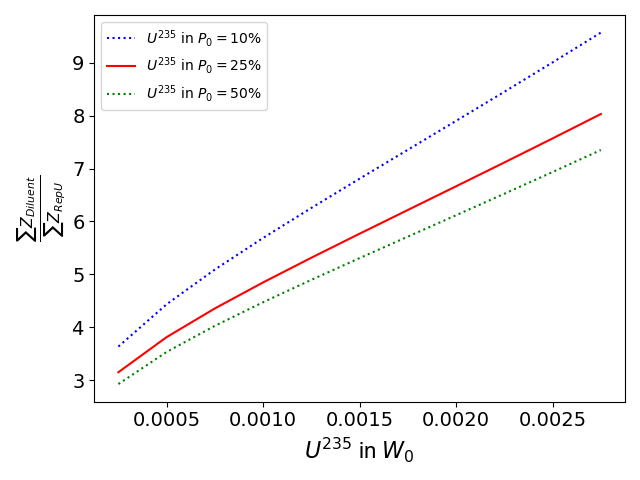
\includegraphics[scale=0.5]{images/plots/myplot}}
%   \caption{Отношение количества центрифуг в каскаде, производящем разбавитель из природного урана, к количеству центрифуг, задействованных для предварительного обогащения регенерата, для различных концентраций $^{235}$U в потоках продукта и отвала каскада, обогащающего регенерат}\label{myplot}
% \end{figure}

Подытоживая анализ результатов вычислительных экспериментов для данной модификации ординарного каскада для обогащения регенерированного урана, можно заключить, что она непригодна для решения задачи обогащения в условиях многократного рецикла, так как с помощью нее нет возможности использовать весь регенерированный уран на производство НОУ-продукта, как показано на рис. \ref{Figure_10}. Однако, такую схему можно использовать для решения задачи повторного использования урана для возврата (дообогащения) регенерата с относительно низким исходным содержанием чётных изотопов, например, в случае обогащения регенерата первого рецикла.


\subsection{Анализ схемы с разбавлением предварительно обогащенного природного урана регенератом}

Проанализируем возможность решения задачи обогащения регенерированного урана со всеми ограничениями в каскадной схеме с разбавлением предварительно обогащенного природного урана регенератом (рис. \ref{o2}). Принцип работы такой схемы состоит в том, что предварительно обогащенный природный уран смешивается с возвращаемым в топливный цикл регенерированным ураном. Уровень предварительного обогащения (перед смешением) природного урана и отношение потоков обогащенного природного урана к регенерату определяются исходя из условий задачи. Таким образом, данная схема в принципе аналогична схеме с разбавлением предварительно обогащенного регенерата природным ураном (рис. \ref{o1}). Это означает, что ей присущи те же недостатки, что и упомянутой схеме, а именно: в ней число управляющих параметров меньше, чем число условий, предъявляемых к конечному продукту. 

\begin{figure}[ht]
  \centerfloat{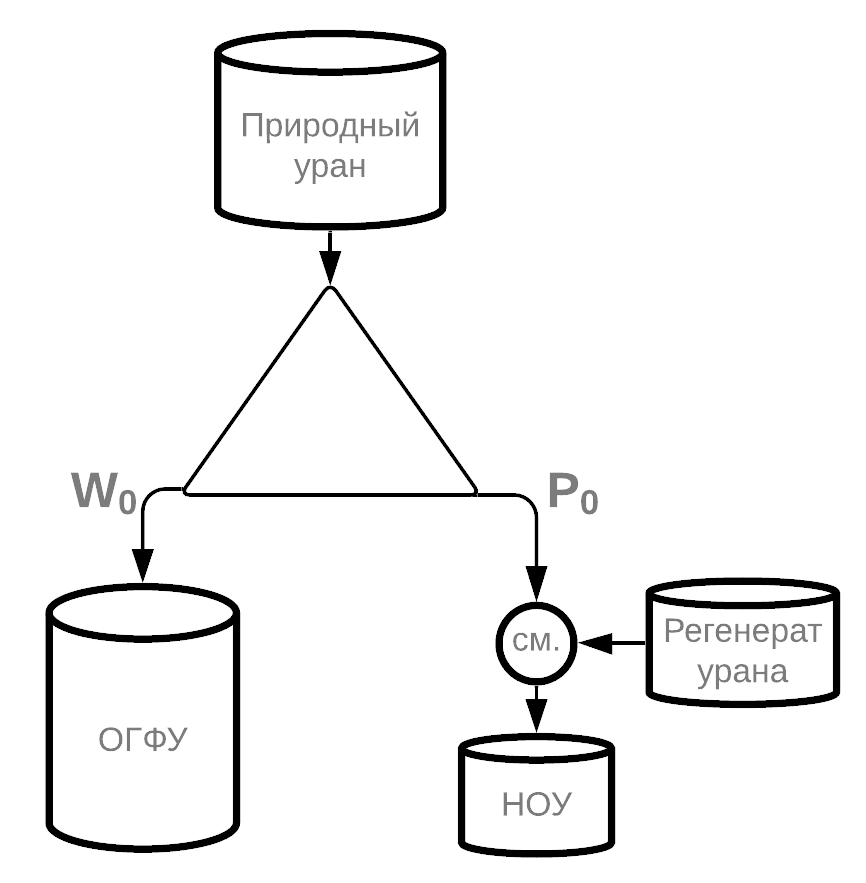
\includegraphics[scale=0.2]{cascades/ordinary/2}}
  \caption{Схема каскада с разбавлением предварительно обогащенного природного урана регенератом. Обозначения: $P_0$ -- поток отбора легкой фракции каскада; $W_0$ -- поток отвального ОГФУ тяжелого <<конца>> каскада; $CM.$ -- узел смешения, на выходе из которого получается конечный НОУ-продукт $НОУ$  -- низкообогащенный уран}\label{o2}
\end{figure}

Для ответа на вопрос о возможности использования данной схемы для обогащения регенерата в условиях многократного рецикла были проведены вычислительные эксперименты, в рамках которых варьировали величину концентрации $^{235}$U в обогащенном природном уране и пропорцию смешивания разбавителя и регенерата с целью найти такой набор параметров схемы, при которых сформулированная в разделе 3.1 задача будет решена. Как и в рассмотренных выше примерах моделирование процесса обогащения урана в каскаде осуществляли с использованием R-каскада. Концентрацию $^{235}$U в отвале каскада задавали равной 0,1\%.

Из результатов вычислительных экспериментов следует, что для рассматриваемой схемы возможно получение решения, удовлетворяющего заданным ограничениям на концентрации изотопов $^{232,234,236}$U. Однако, как и в случае применения схемы рис. \ref{o1}, одновременно с этими условиями не удаётся удовлетворить условие возврата заданной массы регенерата. В результате вместо заданной величины отношения массы исходного регенерата к продукту - 0,93, фактические значения не превысили величины 0,75. Данные результаты свидетельствуют о том, что такая схема обогащения регенерата не решает поставленную задачу для произвольного изотопного состава регенерата и, следовательно, не может быть применена в условиях многократного рецикла урана в топливе легководных реакторов.

\subsection{Анализ схемы с разбавлением регенерата природным ураном перед подачей в ординарный трехпоточный каскад}

Еще одним вариантом каскадной схемы для обогащения регенерированного урана, основанной на использовании ординарного каскада является схема, в которой смешивание и разбавление регенерата происходит непосредственно перед подачей в каскада для последующего обогащения (рис. \ref{o3}). В качестве разбавителя здесь, как правило, рассматривают природный уран. Пропорцию смешивания природного и регенерированного урана определяют, исходя из ограничений на четные изотопы в конечном НОУ-продукте.

\begin{figure}[ht]
  \centerfloat{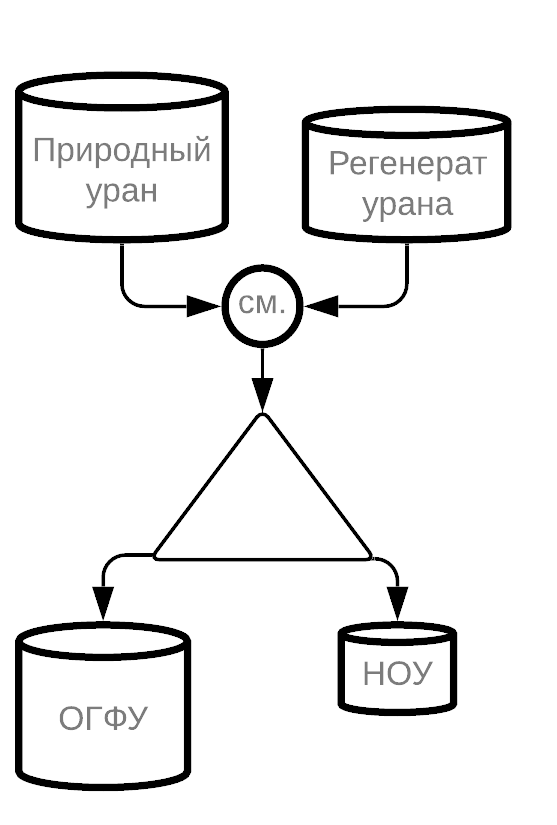
\includegraphics[scale=0.25]{cascades/ordinary/3}}
  \caption{Схема каскада со смешением регенерата и природного урана перед подачей на питание ординарного каскада. Обозначения: см. -- смесь входящих сырьевых потоков, образующих питание каскада; $НОУ$ -- конечный НОУ-продукт схемы}\label{o3}
\end{figure}

В случае, если разбавитель известен, то для такой схемы существует единственный управляющий параметр - это пропорция смешивания регенерата и природного урана. Очевидно, что с ростом доли регенерата в совокупном питании каскада будут возрастать концентрации чётных изотопов в потоке отбора каскада. Это обуславливает тот факт, что существует некоторое критическое значение пропорции, начиная с которого уже невозможно будет соблюсти, как минимум, ограничение на концентрацию изотопа $^{232}$U. Для рассматриваемой схемы также были проведены вычислительные эксперименты, в которых варьировали пропорцию разбавления между регенератом и разбавителем, в качестве которого рассматривали уран природного состава. Как и во всех рассмотренных в рамках данной главы примерах исходные условия соответствовали задачи, описанной в разделе 3.1, а в качестве расчётной модели использован R-каскад. Расчёты проведены на примере состава 1 таблицы \ref{is_compositions_2_5}. 

На рис. \ref{sc3_1.second} отражена взаимосвязь доли регенерата в питании каскада, концентрации $^{232}$U в конечном продукте и отношения потока исходного регенерата к потоку продукта. Кривые построены при различных концентрациях изотопа $^{235}$U в отвале каскада. Как следует из анализа представленных зависимостей, во всех случаях величина концентрации  $^{232}$U достигает предельного значения ($5\cdot10^{-7}$\%) до того, как пропорция между исходным регенератом и продуктом достигнет требуемого значения -- 0,93. Это означает, что и эта схема также не позволяет решить полностью задачу обогащения регенерата с относительно высоким содержанием чётных изотопов. 

\begin{figure}[ht]
  \centerfloat{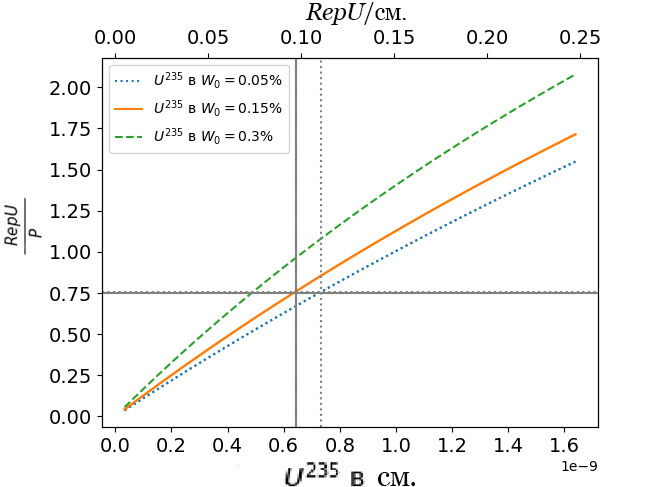
\includegraphics[scale=0.5]{images/plots/3.11new}}
  \caption{Расход регенерированного урана на единицу НОУ-продукта  при различной концентрации $^{232}$U в питающем потоке каскада для различных концентраций $^{235}$U в потоке отвала}\label{sc3_1.second}
\end{figure}


\subsection{Общий вывод для схем возврата регенерата в ЯТЦ на основе ординарного каскада}

Описанные выше результаты вычислительных экспериментов, проведенных для анализа применимости схем на основе простейших модификаций ординарного каскада для решения сформулированной в главе 1 задачи обогащения регенерированного урана, показали что такие схемы не могут решить подобную задачу в условиях  многократного рецикла. Это обусловлено ухудшением изотопного состава урана по мере прохождения им серии топливных циклов, что выражается в накоплении $^{232}$U и других чётных изотопов. При этом исходная концентрация $^{232}$U питающей смеси, начиная со второго рецикла, превышает уровень допустимый в конечном продукте, поэтому схемы, основанные на ординарном каскаде, которые только разбавляют этот изотоп, не эффективны для решения поставленной задачи. Тем не менее, если рассматривать подобные схемы для обогащения регенерированного урана, прошедшего только однократное облучение или допустить "послабление" ограничений на концентрации чётных изотопов, то подобные схемы, безусловно, могут быть применены для решения задачи обогащения регенерированного урана.

При этом закономерно возникает следующий вопрос: возможно ли априорно оценить возможность решить поставленную задачу в таких модификациях ординарного каскада? 

На этот вопрос можно ответить, обратившись к уравнениям баланса компонентов в каскаде \ref{GrindEQ__1_21_} по крайней мере в случае вариантов каскадных схем, где регенерированный уран поступает в каскад для обогащения. Если записать уравнение \ref{GrindEQ__1_21_} для изотопа $^{232}$U и, учитывая, его малую концентрации в исходной смеси сделать предположение о том, что его концентрация в отвале каскада будет стремиться к нулю. Данное предположение может быть вполне оправдано, если отвальная часть каскада имеет достаточное число ступеней. В этом случае $^{232}$U, являясь самым лёгким в смеси регенерированного урана, будет активнее остальных компонентов концентрироваться в отборе каскада. Это означает, что для изотопа $^{232}$U уравнение \ref{GrindEQ__1_21_} можно переписать в следующем виде, пренебрегая слагаемым с потоком отвала каскада:

\begin{equation} \label{GrindEQ__1_21__} 
  \begin{array}{l} {\quad \quad \quad \quad \quad  E+F=P+W,} \\ {FC_{i,F} + EC_{i,E} =PC_{i,P} +WC_{i,W} ,\;  i=1,2,...,m.} \end{array} 
\end{equation} 

\begin{equation}
\label{eq_232_balance}
  C_{232,P} \approx \frac{RepU}{P} C_{232,RepU}
\end{equation}

\begin{equation}
  \label{eq_232_balance_}
    C_{232,P} \approx \frac{E}{P} C_{232,E}
  \end{equation}

Величина $\frac{F}{P}$ в приведенном выше уравнении и является отношением (исходный регенерат)/продукт. Если учесть, что типичные значения этого отношения составляют величину $\approx$0,9-0,95, то станет очевидно, что это условие будет выполнено только, если концентрация $^{232}$U в исходном регенерате ниже, чем ограничение на $^{232}$U в конечном продукте. 
С помощью уравнения \ref{eq_232_balance} можно вычислить максимально возможную долю питающего потока, содержащего $^{232}$U, как неизвестную переменную уравнения \ref{eq_232_balance}. Например, для состава 1 таблицы \ref{is_compositions_2_5}, который был использован в рассмотренных выше примерах получаем:

% \begin{equation}
%   \label{eq_232_balance_X}
%     5 \times 10^{-7} \% \approx X \times 6.622 \times 10^{-7} \% \Rightarrow X \approx 0.755
% \end{equation}

\begin{equation}
  \label{eq_232_balance_X}
    \frac{RepU}{P} \leq 0,755
\end{equation}

\begin{equation}
  \label{eq_232_balance_X_}
    \frac{E}{P} \leq 0,755
\end{equation}

Снова анализируя представленные в предыдущих разделах данные, легко увидеть, что полученные в результате прямого численного расчёта предельные величины отношений (исходный регенерат)/продукт приблизительно и составляют такую величину.
Подобный подход позволяет аналитически оценить возможность применения схем на основе простейших модификаций ординарного каскада, исходя из изотопного состава регенерата. Следует отметить также, что подобные оценки можно также применять и для каскадных схем, в которых регенерат разбавляют уже внутри каскада, путём его подачи в качестве дополнительного питания, поскольку такие схемы по сути являются также только разбавляющими.

\section{Обоснование необходимости составных схем}\label{sec:ch2/sec2}

Как следует из предыдущей части настоящей главы, на текущий момент в принципе имеются способы, позволяющие обеспечить выполнение требований по четным изотопам урана при обогащении регенерата. Однако основной проблемой, решаемой в рамках настоящей диссертационной работы, является поиск варианта каскадной схемы, позволяющей одновременно выполнить ограничения по концентрациям четных изотопов и задействовать в обогащении весь имеющийся регенерат в условиях неопределенности его изотопного состава при многократном рецикле.

Если анализировать причины невозможности возврата массы регенерата в производство топлива в многочисленных модификациях каскада для обогащения многократно облученного регенерата, то становится очевидным, что это, во многом, связано с нарастанием относительных концентраций “легких” изотопов (в первую очередь $^{232}$U) и
$^{235}$U, а поскольку данные изотопы концентрируются вместе на легком <<конце>> каскада, то единственным способом понизить отношение их концентраций -- это разбавить материалом, не содержащим $^{232}$U, например на входе в каскад. Как показали результаты, описанных в этой главе вычислительных экспериментов, для составов с достаточно высоким исходным содержанием $^{232}$U невозможно подобрать такой разбавитель, чтобы удовлетворить одновременно и условие полного возврата массы регенерата в цикл и условия на содержание четных изотопов.

Из приведенного выше анализа следует, что эффективная каскадная схема для обогащения регенерата урана при многократном рецикле должна обеспечивать не только разбавление регенерата, но и хотя бы частичную его очистку от чётных изотопов. Поэтому возможные варианты решения задачи, по-видимому, должны быть основаны на использовании схем двойных каскадов, в том числе, описанных в Главе 1. В связи с этим интерес ответ на вопрос о возможности прямого обогащения регенерата с повышенным содержанием чётных изотопов в двойном каскаде с целью решения задачи обогащения регенерата в наиболее общей постановке. Этот вопрос и рассмотрен в следующих разделах настоящей главы.

\clearpage
           % Глава 2
%\chapter{Решение проблемы возврата регенерированного урана в топливный цикл}

\section{Разработка схем полного возврата}\label{sec:ch2/sec3}
\subsection{Модифицированный двойной каскад}

В качестве модификации двойного каскада была предложена альтернативная каскадная схема, которая позволяет обеспечить возврат регенерата в цикл в требуемом соотношении. В этой схеме, изображенной 
на рисунке \ref{fig:vestnik}, первая часть (каскад 1) увеличивает 
концентрацию $^{235}$U со всеми более легкими изотопами ($^{232}$U и $^{234}$U) и направляет их на вход второго каскада, который, в свою очередь, в легкой фракции будет концентрировать эти четные миноры в потоке загрязненного продукта \cite{smirnovObogashchenieRegenerirovannogoUrana2018}.
Изотопный же состав получаемый на выходе тяжелой фракции второго каскада, разбавляется НОУ-разбавителем, приготовленным из материала, не содержащего четных искусственных изотопов (ранее не облучаемого в реакторе) -- природного или обедненного урана -- для контроля концентраций $^{232}$U и $^{234}$U в допустимых пределах и для управления соотношением рециклируемых материалов (для поддержания соотношения регенерата в питании каскада к нарабатываемому продукту на требуемом уровне, который формально соответствует эквивалентному возврату (1:1) выгоревшего топлива в ядерный топливный цикл).

\begin{figure}[ht]
  \centerfloat{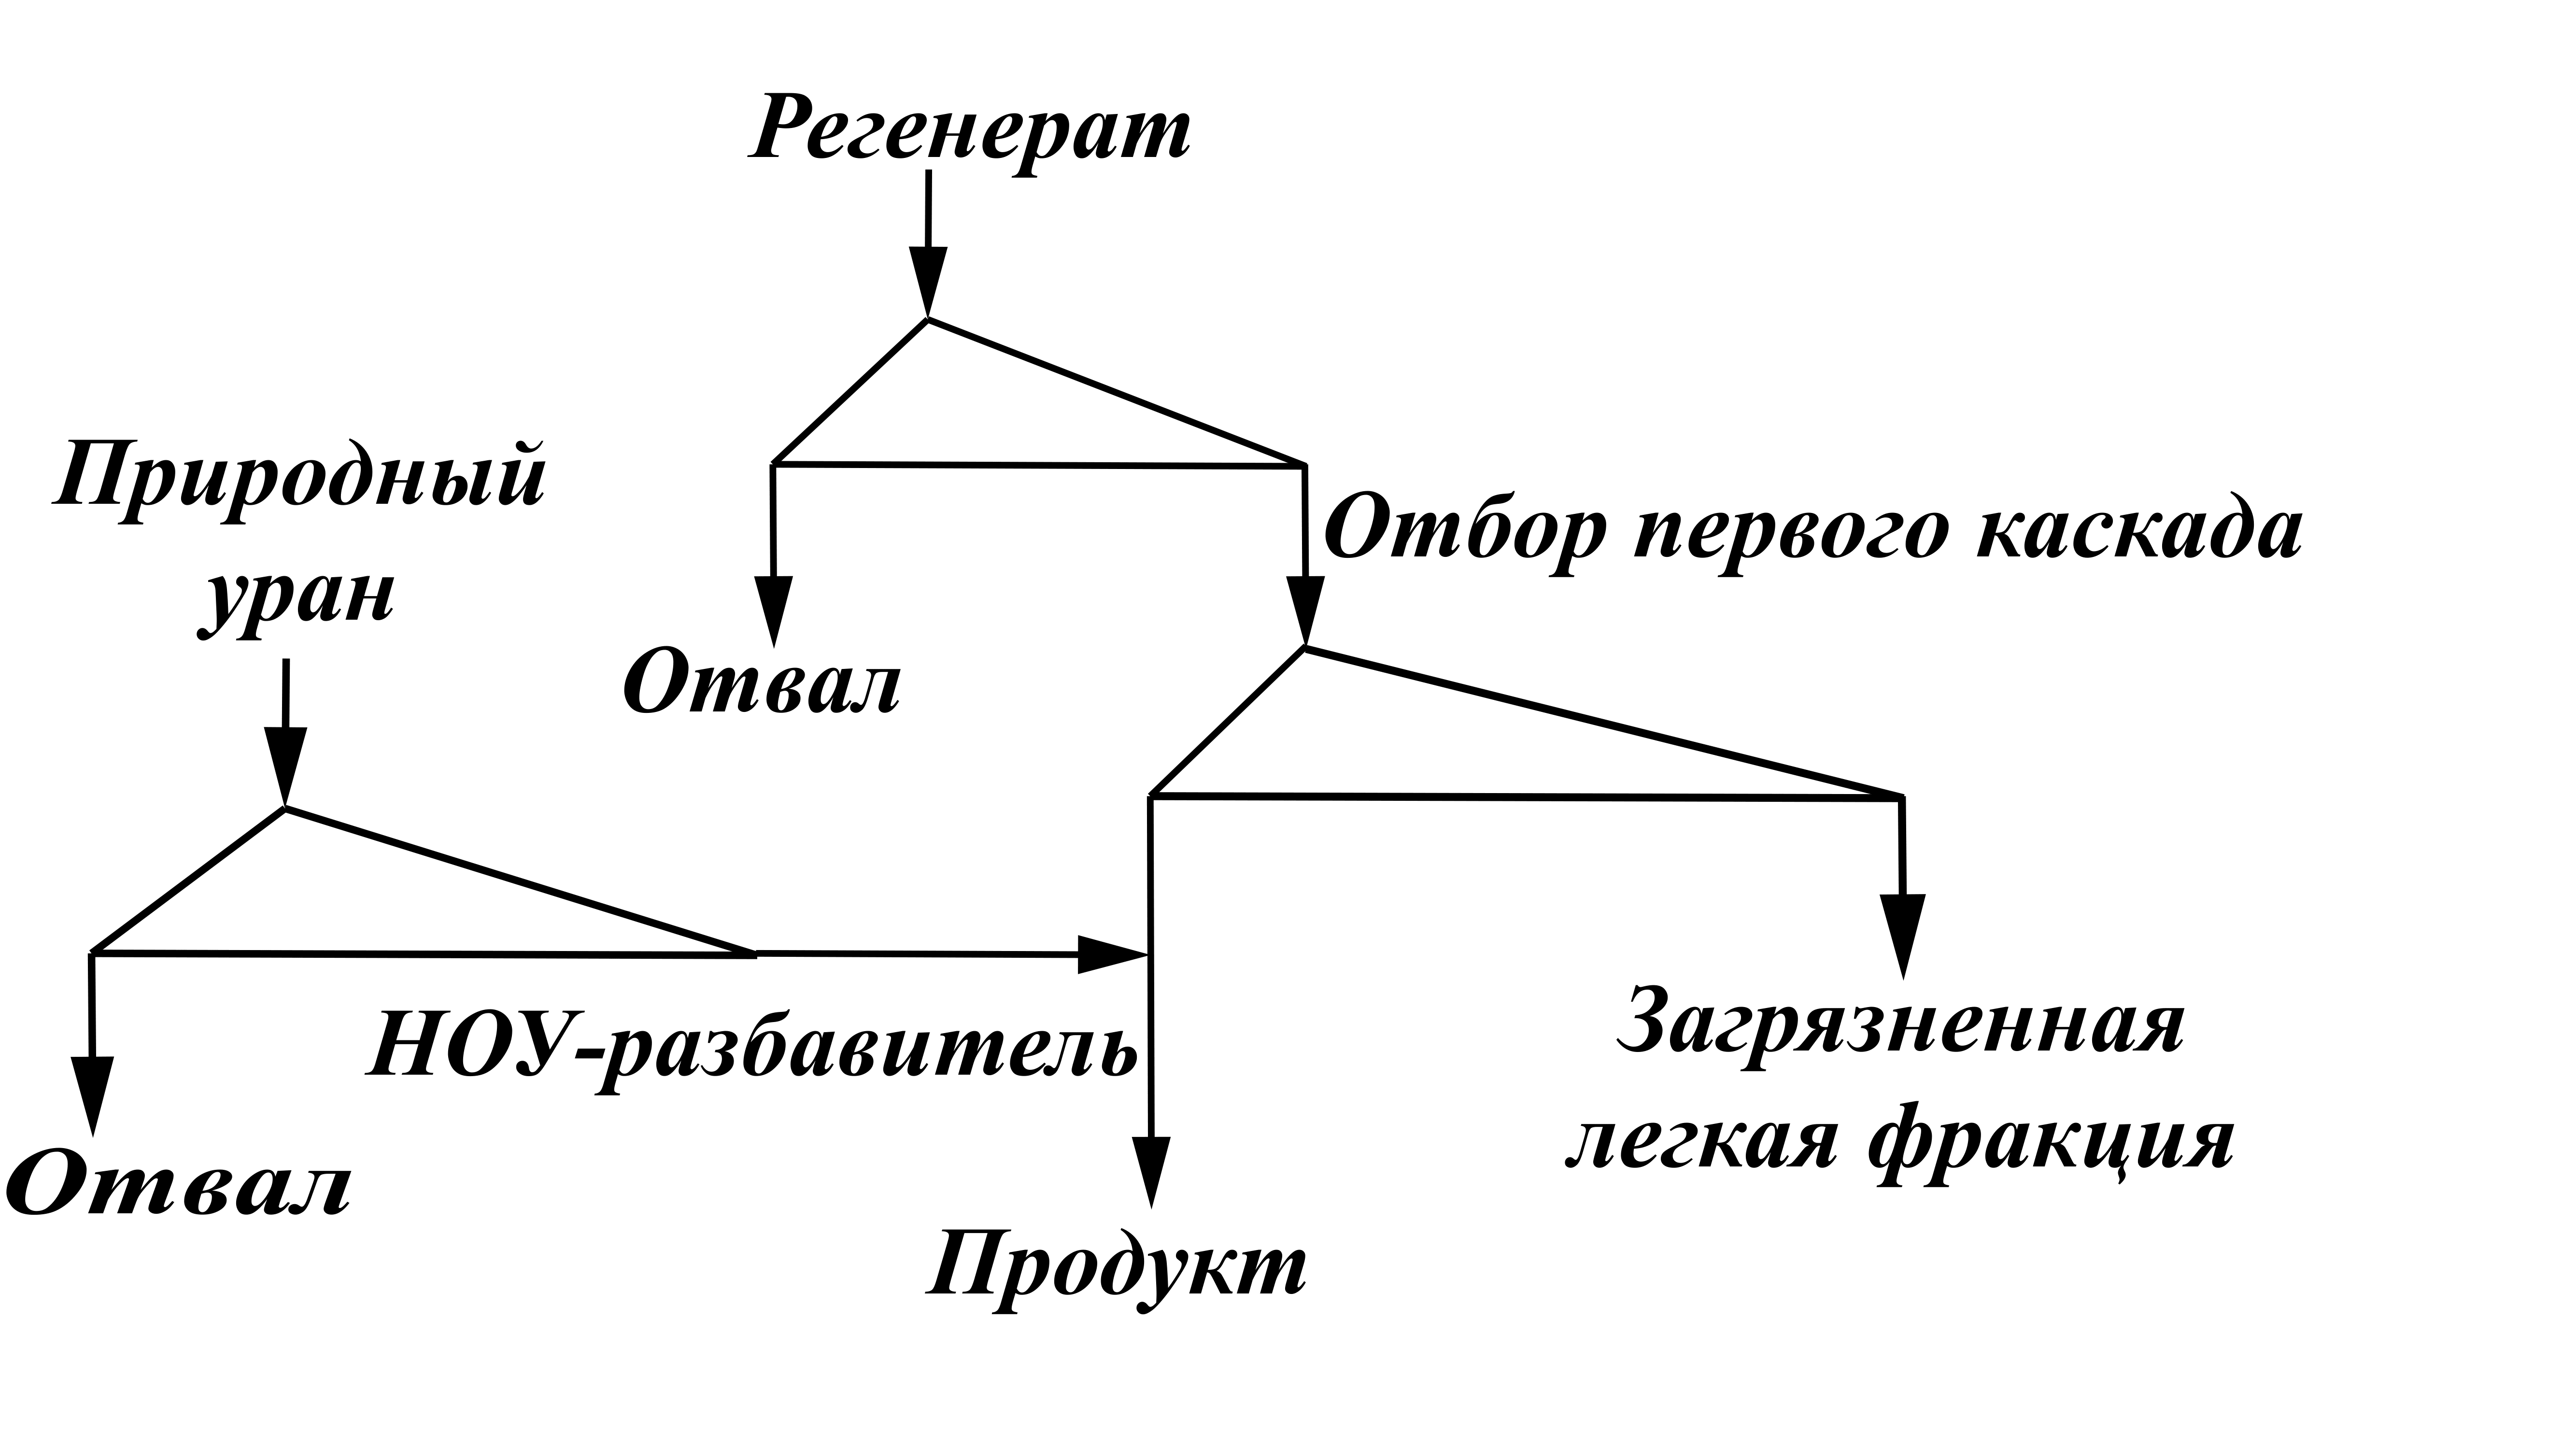
\includegraphics[scale=0.08]{cascades/triple}}
  \caption{Двойной каскад с добавлением НОУ (тройной каскад)}\label{fig:vestnik}
\end{figure}

Отличие предлагаемой схемы от двойного каскада (рис. \ref{fig:double_ru}) состоит в том, что поток отвала второго каскада не является конечным продуктом.
Финальным шагом получения товарного продукта является разбавление этого потока сырьём, не содержащим искусственных изотопов урана с целью их разбавления и, соответственно, обеспечения заданных ограничений по $^{232,236}$U.
Для выполнения условия полного возврата регенерата в цикл, отношение потоков НОУ-разбавителя и отвала второго каскада, которые образуют товарный продукт, является предопределённым, поскольку при заданной концентрации выходящих потоков обоих каскадов известным является отношение потока тяжелой фракции второго каскада к питающему регенерату, и при этом условиями задачи предопределено отношение потока исходного регенерата к конечному-НОУ.
В этом случае единственным параметром, позволяющим влиять на концентрацию $^{235}$U в товарном продукте, является концентрация данного изотопа в разбавителе (в потоке НОУ-разбавитель на рис. \ref{fig:vestnik}).
Таким образом, величину обогащения $^{235}$U в потоке этого разбавителя подбирают для конкретных заданных внешних условий \cite{smirnovObogashchenieRegenerirovannogoUrana2018}.

Очевидно, что, поскольку питанием первого каскада является исходный регенерат, а питанием второго -- полученный из него среднеобогащённый регенерат, то поток тяжёлой фракции на выходе из второго каскада будет по величине в несколько раз меньше, чем исходный поток регенерата. Такая работа каскада обеспечивает перерасход регенерата на единицу продукта. Следовательно, поток разбавителя должен в несколько раз превосходить по величине поток тяжелой фракции второго каскада. Однако, если в качестве разбавителя использовать, например, природный уран, это условие может привести к снижению концентрации $^{235}$U ниже требуемой величины. Если же в качестве разбавителя использовать низкообогащённый уран, то можно увеличить отношение потоков НОУ-разбавителя к <<отвалу>> второго каскада, доведя ее до требуемого значения.  
Такая схема близка к описанной в патенте \cite{zhurinSposobIzotopnogoVosstanovleniya2010}. Однако отличием предлагаемого двойного каскада является то, что ни в одном из каскадов в схеме не происходит превышение концентрации $^{235}$U выше значения 20\%. При этом в схеме  \cite{zhurinSposobIzotopnogoVosstanovleniya2010} концентрация $^{235}$U в потоке P1 достигает 90\% и более. Кроме того, величина отношения потока регенерата к конечному продукту на рис. \ref{fig:vestnik} всегда является строго заданной, что позволяет расходовать на получение заданного количества продукта требуемое количество регенерированного урана.

Итак, согласно \cite{smirnovObogashchenieRegenerirovannogoUrana2018} схема, представленная на рис. \ref{fig:vestnik}, позволяет обогатить регенерированный уран, полученный после пяти рециклов в топливе реакторов ВВЭР-1000 при соотношении расхода регенерата и продукта 0,93 и ограничении на концентрацию $^{232}$U соответствующему значению $5\cdot10^{-7}$\%. Представляет интерес анализ возможности обогащения регенерата в такой схеме при заданном соотношении между массами исходного регенерата и продукта больше единицы. Такое заданное условие моделирует ситуацию обогащения и вовлечения в воспроизводство топлива регенерированного урана, накопленного к текущему моменту за период эксплуатации легководных реакторов. Дополнительный интерес представляет анализ поведения характеристик подобной схемы в зависимости от ограничений на концентрацию изотопа $^{232}$U в продукте. 

\subsubsection{Анализ влияния ограничений предельно допустимой концентрации $^{232}$U в товарном НОУ}

Далее представлены результаты расчёта параметров модификации двойного каскада, представленной на рис. \ref{fig:vestnik}, для различных ограничений на концентрацию изотопа $^{232}$U в продукте, а также соотношения между расходами исходного регенерата и получаемым товарным НОУ.
Согласно цели диссертации, состоящей в исследовании возможностей полного возврата регенерата в режиме многократного рецикла, в качестве сырья для обогащения был рассмотрен регенерированный уран, испытавший несколько циклов облучения (табл. \ref{244549}) \cite{palkinDesignanalyticalResearchRefinement2010}.

Расчёты проведены при следующих условиях: обогащение по изотопу $^{235}$ составляло 4,95\%; относительный коэффициент разделения компонентов $^{235}UF_6$ и $^{238}UF_6$ принят равным 1,2 \cite{smirnovObogashchenieRegenerirovannogoUrana2018}; предельно допустимая концентрация изотопа $^{232}$ в НОУ не должна превышать величины $5\cdot10^{-7}$\%, $2\cdot10^{-7}$\%,$1\cdot10^{-7}$\%; потеря реактивности из-за присутствия $^{236}$U скомпенсирована добавочным обогащением по $^{235}$U; рассматривался состав обогащаемого регенерированного урана пятого рецикла \ref{244549}. Заданный расход регенерированного урана на единицу продукта принят равным:
а) 0,93 кг на 1 кг,
б) 1,86 кг на 1 кг продукта.
Цели расчетов:
\begin{enumerate}
  \item оценка возможности применения рассматриваемой схемы для указанных условий;
  \item оценка влияния изменения внешних условий на интегральные параметры рассматриваемого двойного каскада.
\end{enumerate}

В качестве расчётной модели в настоящей работе использована модель <<квазиидеального>> каскада \cite{sazykinKvaziidealnyeKaskadyDlya2000} с несмешиванием по относительным концентрациям выбранной пары компонентов (R-каскада) \cite{sulaberidzeTeoriyaKaskadovDlya2011}.
Ключевые интегральные характеристики для сравнения: удельный расход природного урана, удельные затраты работы разделения и отношение потока легкой фракции второго каскада к конечному продукту. В приведённых ниже результатах под работой разделения имели в виду условную величину, пропорциональную числу газовых центрифуг в каскаде. 

При этом в каждом каскаде были выбраны следующие пары компонентов, по которым было выполнено условие несмешивания их относительных концентраций: первый каскад $^{235}U$/$^{236}U$, второй каскад $^{235}U$/$^{234}U$.

Концентрацию $^{235}U$ в потоке $P_1$ варьировали в пределах 5--20\% с шагом 1\%, в качестве рабочего значения для каждого случая выбирали величину, обеспечивающую выполнение ограничения на содержание $^{235}U$ в разбавителе, полученном из природного урана, не более 5,0\%. Для такого значения будет наблюдаться минимум по затратам работы разделения, экономии природного урана и отношению потоков $\frac{P_2}{P_0}$. Последнее условие означает, что будет произведено наименьшее количество загрязнённого $^{232}U$, $^{234}U$ изотопами материала $P_2$, хранение которого требует определённых процедур, поскольку он представляет собой повышенную по отношению к штатным отходам разделительных производств опасность.

В табл. \ref{table_PDK_double_modified} представлены результаты расчёта изотопных составов,
в табл. \ref{table3_PDK_double_modified} -- удельный расход природного урана и интегральные характеристики экономии природного урана и перерасхода работы разделения по сравнению с ординарным каскадом, питаемым природным ураном, получающим продукт с эквивалентной эффективной концентрацией $^{235}$U (табл. \ref{table3_PDK_double_modified}). Под работой разделения понимается условная величина, пропорциональная числу газовых центрифуг в каскаде.
 Далее представлены соотношения получаемого загрязненного потока легкой фракции второго каскада к итоговому продукту.

\begin{table}
\begin{tabular}{|c|c|c|c|}
  \hline \multirow{2}{*} {Maccoвoe число} & 
  \multicolumn{3}{|c|}
  {Ограничение по изотопу $^{232} \mathrm{U}$, $\times 10^{-7}$} \\
  \cline {2-4} & 1 & 2 & 5 \\
  \hline \multicolumn{4}{|c|} {Случай $1\left(E_{1} / P_{0}=0,93\right)$} \\
  232 & $1,00 \cdot 10^{-7}$ & $2,00 \cdot 10^{-7}$ & $5,00 \cdot 10^{-7}$ \\
  233 & $2,12 \cdot 10^{-7}$ & $3,62 \cdot 10^{-7}$ & $7,41 \cdot 10^{-7}$ \\
  234 & $4,90 \cdot 10^{-2}$ & $5,30 \cdot 10^{-2}$ & $6,21 \cdot 10^{-2}$ \\
  235 & 5,06 & 5,09 & 5,14 \\
  236 & $3,70 \cdot 10^{-1}$ & $4,67 \cdot 10^{-1}$ & $6,61 \cdot 10^{-1}$ \\
  \hline \multicolumn{4}{|c|} {Случай $2\left(E_{1} / P_{0}=1,86\right)$} \\
  232 & $1,00 \cdot 10^{-7}$ & $2,00 \cdot 10^{-7}$ & $5,00 \cdot 10^{-7}$ \\
  233 & $2,40 \cdot 10^{-7}$ & $4,12 \cdot 10^{-7}$ & $8,55 \cdot 10^{-7}$ \\
  234 & $5,09 \cdot 10^{-2}$ & $5,60 \cdot 10^{-2}$ & $6,79 \cdot 10^{-2}$ \\
  235 & 5,10 & 5,15 & 5,24 \\
  236 & $5,26 \cdot 10^{-1}$ & $6,73 \cdot 10^{-1}$ & $9,85 \cdot 10^{-1}$ \\
  \hline
  \end{tabular}
  \caption{Изотопные составы продукта в модифицированном двойном каскаде для различных условий}\label{table_PDK_double_modified}
\end{table}

\begin{table}
\begin{tabular}{|c|c|c|c|c|}
  \hline
  \makecell{$^{235}$U в \\ потоке  \\ отбора  \\первого  \\каскада, \%} & \makecell{Экономия \\природного  \\ урана, \%} & \makecell{Перерасход \\ работы  \\ разделения, \%} & \makecell{Отношение \\ потока  отбора \\второго каскада \\ к продукту}
  & \makecell{Ограничение  \\ по изотопу $^{232}$U \\ , $\times 10^{-7}$} \\
  \hline
  \multicolumn{5}{|c|} {Случай $1\left(E_{1} / P_{0}=0,93\right)$} \\
  11 & 4,9 & 17,2 & 0,02785 & 1 \\
  10 & 6,7 & 14,7 & 0,02201 & 2 \\
  8 & 10,3 & 9,7 & 0,01038 & 5 \\
  \multicolumn{5}{|c|} {Случай $2\left(E_{1} / P_{0}=1,86\right)$} \\
  13 & 6,6818 & 39,0985 & 0,06648 & 1 \\
  12 & 9,2857 & 35,4797 & 0,05798 & 2 \\
  10 & 14,7795 & 27,7759 & 0,04005 & 5 \\
  \hline
  \end{tabular}
  \caption{Интегральные параметры рассматриваемого двойного каскада для различных внешних условий}\label{table3_PDK_double_modified}
\end{table}


Анализ результатов таблицы \ref{table_PDK_double_modified}  показывает, что рассматриваемая модификация двойного каскада позволяет многократно обогатить регенерированный уран при различных внешних ограничениях, касающихся концентрации $^{232}$U в продукте и величины потока возвращаемого в воспроизводство топлива регенерированного урана.
При этом уменьшение допустимой концентрации $^{232}$U в продукте при фиксированном отношении исходного регенерата к товарному НОУ обусловливает существенное снижение экономии природного урана и изменение числа центрифуг в каскадной схеме.
Например, при отношении регенерата к конечному продукту на уровне 0,93 экономия природного урана уменьшилась, а перерасход работы разделения увеличился примерно в 2 раза при изменении ограничения на $^{232}$U от $5\cdot10^{-7}$\% до $1\cdot10^{-7}$\%. Однако введение более жёстких ограничений на $^{232}$U способствовало одновременному снижению концентрации и остальных чётных изотопов в получаемом продукте, особенно $^{236}$U. Данный фактор является положительным в случае многократного рециклирования урана, поскольку будет обеспечивать меньшее содержание $^{232}$U на последующих рециклах \cite{smirnovObogashchenieRegenerirovannogoUrana2018}.

В рамках настоящей работы рассматривали случай, когда данная концентрация не превышала 20\%, что соответствует порогу, принятому МАГАТЭ для материала прямого использования \cite{alekseevConceptUseRecycled2010}. Однако в некоторых работах, в которых рассматривают двойные каскады для обогащения регенерата, указанная концентрация заметно (в 2 раза и более) превышает величину 20\%. Увеличение данной концентрации, возможно, позволит уменьшить количество получаемого радиоактивного отхода, а также обеспечить более эффективное удаление $^{232}$U из продукта.

Таким образом, использование модифицированного двойного каскада с добавленным потоком НОУ-разбавителя для перемешивания с одним из выходящих потоков второго каскада позволяет успешно обогащать многократно рециклированный уран с максимальным возвратом его в воспроизводство при различных ограничениях на концентрацию изотопа $^{232}$U в продукте, включая более строгие ограничения, чем приняты в настоящее время на заводах по фабрикации топлива для реакторов на тепловых нейтронах.

Хотя этот вариант каскада (рис. \ref{fig:vestnik}) и кажется идеальным, цена хранения побочного продукта из загрязненной смеси может быть неприемлемо высока, что мгновенно сделает схему нежизнеспособной, если нет способов избежать такого негативного побочного эффекта.

\subsection{Тройной каскад}
Итак, в прошлом подразделе, в качестве необходимой модификации двойного каскада была предложена схема каскада рис. \ref{fig:vestnik}, которая позволяет решить проблему возврата необходимого количества регенерата в цикл.

Хотя этот вариант и кажется подходящим для решения поставленной задачи, остается нерешенной судьба легкой фракции второго каскада из-за того, что хранение загрязненного побочного продукта может быть сопряжено с существенными дополнительными затратами, поэтому важен поиск способов избежать накопления этого материала.
Исходя из этого, в диссертационной работе предложено применить дополнительный каскад для утилизации потока загрязненной фракции.

Далее будет предложен краткий обзор такой каскадной схемы.
 
Итак, в \cite{smirnovMethodEnrichReprocessed2019}  было предложено применять дополнительный каскад для производства НОУ из загрязненной смеси, сильно разбавленной обедненным ураном (которые имеют высокую концентрацию $^{235}$U около $\approx$20\%), чтобы получить конечный продукт в двух исходящих потоках и достичь значительной экономии природного урана ($\approx$38\%) даже для <<грязной>> композиции, которая уже была пятикратно рециклирована (рис. \ref{fig:Tomsk}). Расчеты показали, что такой подход позволяет производить НОУ коммерческого качества, расходуя определенное количество переработанного урана и отвечая стандартным спецификациям для  $^{232}$U (и условиям, установленным для других четных изотопов). В то же время, предлагаемая схема обеспечивает большую экономию природного урана, чем большинство схем обогащения переработанного урана. Это могло бы также обеспечить широкомасштабную <<мобилизацию>> обедненного урана.

\begin{figure}[ht]
  \centerfloat{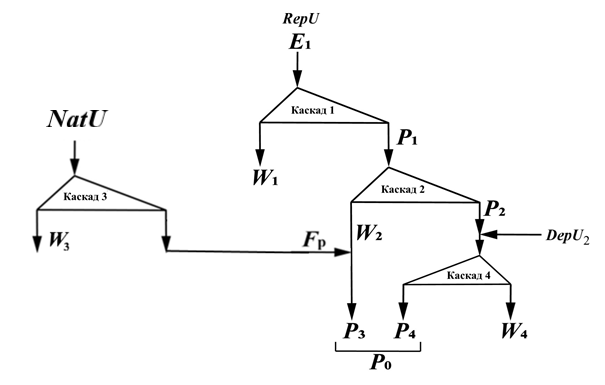
\includegraphics[scale=0.9]{cascades/triple_t}}
  \caption{Тройной каскад с подмешиванием ОГФУ и НОУ-разбавителем}\label{fig:Tomsk}
\end{figure}

Схема такого каскада, состоящего из четырех ординарных каскадов, решает проблему обращения с легкой фракцией, вышедшей из второго каскада.
Это позволяет вовлечь больше $^{235}$U, и избавляет от необходимости конечной утилизации материала с высоким содержанием $^{232}$U.
Принцип работы такой схемы состоит в следующем.
Теперь финальный продукт -- низкообогащенный уран -- получается путем смешения двух потоков.
Первый из них аналогичен финальному продукту, полученному посредством двойного модифицированного каскада.
Второй же нарабатывается из загрязненной смеси, сильно разбавленной обедненным ураном.
При этом, конфигурация подбирается таким образом, чтобы на получение единицы продукта из этих совмещенных потоков затрачивалось требуемое количество ($\approx$0.93) питающего регенерата.

Итак, данная схема позволяет получить конечный НОУ-продукт требуемого качества, смешав два производящих потока и достичь значительной экономии природного урана ($\approx$38\%) даже для «грязного» регенерата, который уже  пятикратно был рециклирован.
При этом, для того же исходного состава регенерата, схема двойного модифицированного каскада (рис. \ref{fig:vestnik}) показывает лишь ($\approx$8\%) в сокращении расхода природного урана в сравнении с ординарным, обогащающим природный уран \cite{smirnovObogashchenieRegenerirovannogoUrana2018}.
Однако, такой эффект связан с двухкратным перерасходом работы разделения в схеме тройного каскада, тогда как в схеме двойного модифицированного каскада затрачивается лишь ($\approx$13\%) дополнительной работы разделения.
Это связано с большим объемом вовлечения ОГФУ для разбавления загрязненного потока легкой фракции второго каскада.
Расчеты показали, что такой подход позволяет производить НОУ коммерческого качества, расходуя должное количество переработанного урана, в то же время отвечая стандартным спецификациям $^{232}$U (и условиям, установленным для других четных изотопов).
В то же время, предлагаемая схема обеспечивает более существенную экономию природного урана, чем большинство схем обогащения регенерированного урана.
Такая схема позволяет также обеспечить широкомасштабную «мобилизацию» обедненного урана.

\section{Сравнение схем полного возврата}

Чтобы проиллюстрировать преимущества и недостатки различных рассмотренных ранее схем, предназначенных для возврата регенерированного урана в ЯТЦ, в данной части диссертационной работы проводится их сравнительный анализ, помогающий сделать предварительные технико-экономические оценки.
Для этого, ключевые характеристики, связанные с общей эффективностью, такие как экономия природного урана, расход работы разделения и энергозатраты, были оценены для каждой схемы в удельных единицах (на единицу продукции).
Затем они были нормированы на величины, характерные для ординарного каскада(трехпоточного).
Чтобы избежать стоимостных показателей затрат, была использована методология пересчета ключевых показателей (экономия природного урана, объем обогащаемого ОГФУ и затраты работы разделения) в единицы потребляемой энергии (мегаватт-часы)  \cite{rodionovaAnalizTehnikoekonomicheskihHarakteristik2019}.
Этот показатель и был предложен в качестве универсального инструмента оценки рассматриваемых каскадов, используемых для повторного обогащения урана.

Концентрация $^{235}$U в потоках отбора второго каскада ограничена уровнем 19,99\% (чтобы не превышать пороговое значение концентрации $^{235}$U для низкообогащенного урана). Для каждого каскада с индексом 2 опорный компонент составляет $^{236}$U и $^{238}$U -- для остальных каскадов.

В качестве схемы №1 рассматривается двойной каскад (рис. \ref{fig:double_ru}), в качестве схемы №2 -- двойной модифицированный (рис. \ref{fig:vestnik}), а в качестве схемы №3 -- тройной каскад (рис. \ref{fig:Tomsk}), для которого подбирается уровень перерасхода работы разделения на уровне 25\% и 50\%, относительно ординарного каскада, обогащающего природный уран для аналогичных значений $^{235}$U.
\begin{table}[h]
  \begin{center}
  \begin{tabular}{|c|c|c|c|c|c|}
  \hline
  \makecell{Схема, №} & \makecell{Экономия  \\ природного  \\ урана,\% }
  & \makecell{Перерасход \\ работы  \\ разделения, \%}
  & \makecell{Расход  \\ регенерата  \\ на единицу \\  продукта}
  & \makecell{Расход  \\ ОГФУ \\  на  \\ единицу \\  продукта} & \makecell{Относительная  \\ стоимость, \%} \\
  \hline
  1&100&41.63&8.26&0&0.32\\
  2&10.07&6.08&0.93&0&89.96\\
  3&15.08&25&0.93&31.11&85.00\\
  3&23.13&50&0.93&74.49&77.02\\
  \hline
  \end{tabular}\caption{Интегральная таблица характеристик сопоставляемых каскадных схем.}\label{4comp}
  \end{center}
\end{table}

Несмотря на 100\% экономию природного урана и, следовательно, низкую относительную стоимость, схема №1  -- двойной каскад -- (рис. \Ref{fig:double}) не соответствует требованиям к содержанию $^{232}$U в конечном продукте.\\
Поэтому результаты, которые показывают, что выигрыш в экономии природного урана (и, как следствие, в относительной себестоимости) обусловлен лишь незначительным дополнительным расходом работы разделения, не могут считаться удовлетворительными.
Рассмотренные схемы, кроме №1, производили НОУ заданного реакторного качества, обеспечивая при этом требуемую пропорцию расхода регенерата на единицу продукта.
Схемы же №3и №4 (рис. \ref{fig:vestnik},\ref{fig:Tomsk}) могут обеспечить желаемое соотношение потребления регенерата на единицу продукта, а №4 (рис. \ref{fig:Tomsk}) демонстрирует наилучшие результаты в сохранении природного урана, которые могут быть еще увеличены с помощью дополнительной работы разделения (с более полным извлечением $^{235}$U при удлинении обеднительных частей каскадов).
И, как ранее было отмечено, схема №4 является единственной схемой из рассмотренных, которая предотвращает накопление токсичных отходов (изотопный состав с высоким содержанием $^{232}$U и $^{235}$U).
Однако, сопутствующая <<мобилизация>> обедненного урана хоть и может иметь дополнительные преимущества, поскольку складские запасы этого материала сами по себе являются проблемой, она требует дополнительных затрат работы разделения\cite{fitchOPTIONSDISPOSALREAPPLICATION2009}.
При рассмотренном критерии себестоимости, соответствующим энергозатратам на единицу НОУ, увеличение разделительной работы сопровождается снижением себестоимости, так как сэкономленный уран вносит самый значительный вклад в изменение этого показателя \cite{gusevMultycascadeEnrichmentSchemes2020}. \\
Отсюда можно сделать вывод, что каскадная схема №4 (рис. \ref{fig:Tomsk}) являетсянаиболее предпочтительной для решения задачи возврата регенерата в ЯТЦ в многократном рецикле, в условиях, когда используется способ стоимостной оценки, отдающий предпочтение экономии природного урана.

Недостаток способа состоит в том, что такой подход хоть и позволяет на 100\% решить проблему с накоплением загрязненных $^{232}$U отходов, вынуждает использовать значительные объемы ОГФУ.

% Поэтому, в качестве альтернативы была предложена схема рисунка \ref{fig:patent}), в которой на каскад с индексом 3 подается смесь грязного потока легкой фракции каскада 2, которая разбавляется обедненным гексафторидом урана до содержания $^{235}$U на уровне природного урана. Этот поток в дальнейшем разбавляется чистым природным ураном, пропорция которого подбирается для выполнения всех заданных условий.
% \begin{figure}[ht]
%   \centerfloat{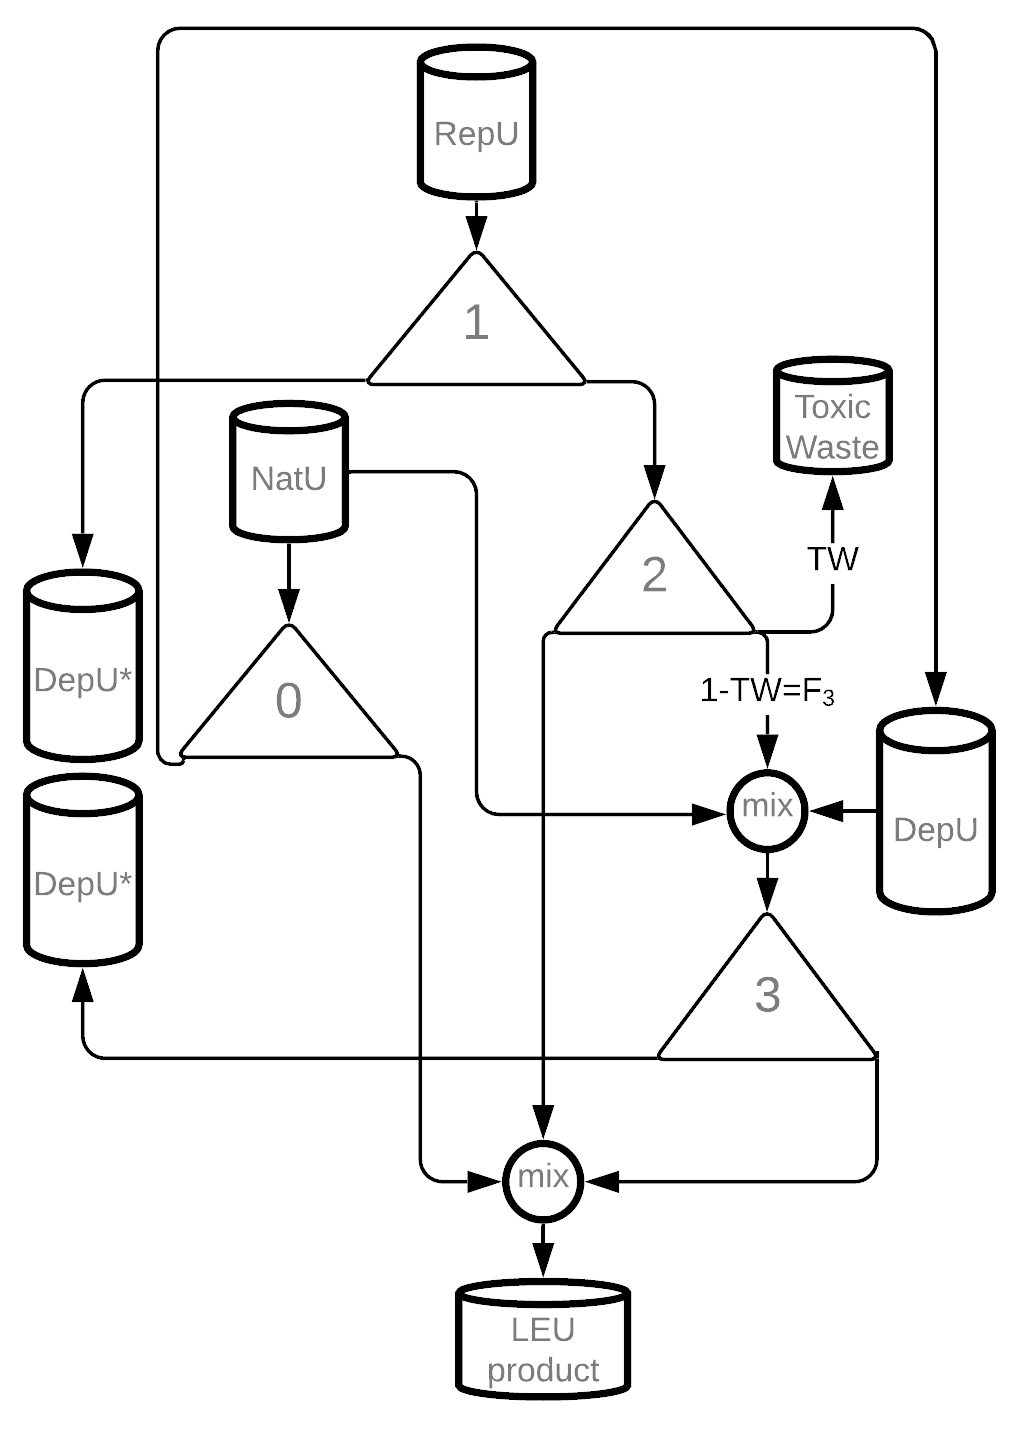
\includegraphics[scale=0.3]{cascades/triple_cascade_complete_return}}
%   \caption{Тройной каскад с подмешиванием НОУ, ОГФУ и природного урана}\label{fig:patent}
% \end{figure}

% Как мы видим, такие схемы также очень ценны как инструмент для переработки предписанного количества выделенного из ОЯТ урана.

Так как наиболее ценны схемы, которые решают вопрос включения побочной легкой фракции в производство свежего НОУ, в качестве альтернатив могут быть рассмотрены следующие схемы.

Одним из вариантов утилизации побочной легкой фракции, образующейся во втором каскаде схемы рис. \ref{fig:vestnik}, является возможность смешать этот побочный продукт с обедненным ураном и отправить на последующее длительное хранение \cite{vodolazskihSposobIzotopnogoVosstanovleniya}. Здесь поток легкой фракции второго каскада разбавляется обедненным гексафторидом из имеющихся складских запасов (дважды обедненным, с низким содержанием $^{235}$U $\approx$0,1\%), отправляя полученную ядерно-безопасную смесь на длительное хранение. Недостатки этого метода заключаются в том, что, хотя этот подход позволяет полностью решить проблему накопления загрязненных отходов $^{232}$U, он вынуждает использовать значительные объемы обедненного гексафторида (в $\approx$50 раз больше, чем разбавляемая им изотопная смесь), а также как тот факт, что значительная масса целевого изотопа $^{235}$U будет потеряна для возможности применения в производстве свежего НОУ, что снизит эффективность использования переработанного урана, которая выражается в степени извлечения $^{235}$U из регенерата. Степень извлечения этого изотопа для схемы двойного модифицированного каскада может быть записана как
$U^{235}_{Rec} = \frac{P \cdot C_{P}^{235}}{F_0 \cdot C_{NatU}^{235} + E \cdot C_{E}^{235}}$, где массовые потоки $P$, $E$ и $F_0$ умножены на концентрации $^{235}$U в этих потоках.

Тогда как в таком варианте предлагается избавиться от радиоактивного материала с высокой концентрацией $^{232}$U путем разбавления его обедненным гексафторидом и последующей отправкой на хранение, помимо методов, позволяющих избежать его накопления, применяя его для конечного производства НОУ, таких как тройные схемы \cite{smirnovMethodEnrichReprocessed2019}, существует вариант направить поток легкой фракции на питание другого двойного каскада, производящего НОУ для последующего цикла \cite{nevinicaToplivnyyCiklLegkovodnogo2019}. Такую схему  каскада целесообразно использовать в условиях многократного рецикла урана, начиная со второго рецикла, а также в условиях постоянного производства регенерированного топлива для парка реакторов на тепловых нейтронах. Устройство этой схемы, изображенной на рис. \ref{P2utilizationRing} предлагает вовлекать этот материал после его накопления в результате обогащения изначальной партии регенерата $E$, поступившей на обогатительное производство в обогащение следующей партии регенерированного урана $E'$ из переработанных ОТВС. Показано, что реализация предлагаемой схемы позволяет полностью израсходовать как вновь поступивший на повторное обогащение регенерированный уран, так и проблемный промежуточный продукт $P_2$, оставшийся после прошлой операции по дообогащению -- гексафторид высокообогащенного урана с относительно высоким содержанием $^{232}$U.

\begin{figure}[ht]
  \centerfloat{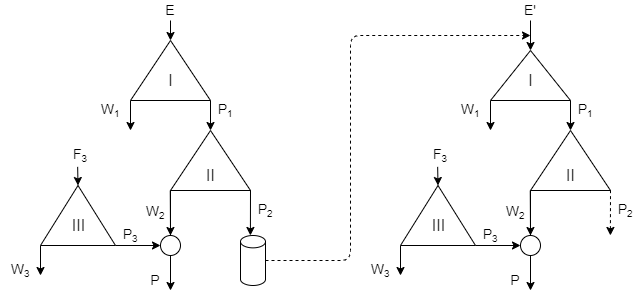
\includegraphics[scale=0.7]{cascades/P2utilizationRing}}
  \caption{Схема передачи загрязненной изотопом $^{232}$U фракции гексафторида урана в двойном каскаде от первой партии дообогащенного регенерированного урана к последующей.}\label{P2utilizationRing}
\end{figure}

Процесс возврата данного материала в воспроизводство низкообогащенного урана может быть начат практически после дообогащения регенерата уже для одной ТВС и даже для ее части (непрерывный возврат), схема каскада при этом преобразуется к виду, когда проблемный промежуточный продукт $P_2$ возвращается и подмешивается к потоку питающего исходного регенерата $E$.

Очевидно, что при использовании предлагаемой схемы и непрерывной работе завода по обогащению, удастся полностью замкнуть топливный цикл по урану, а единственным отходом производства станет только обедненный гексафторид, образующийся в отвале первого каскада. Однако данный продукт можно считать штатным отходом
обогатительного производства, для которого на сегодняшний день отработаны технологии хранения и переработки. При этом после вывода завода из эксплуатации (или остановки на планово-предупредительный ремонт) останется невостребованным только тот объем обогащенного по изотопу $^{232}$U гексафторида урана, который будет образован после обогащения последней партии регенерата на этом заводе. Таким образом, предлагаемый в настоящей статье подход к дообогащению регенерата урана позволяет организовать полный возврат регенерированного урана в топливный цикл в течение практически всего жизненного цикла топлива легководных реакторов,
работающих в замкнутом топливном цикле, как показывают результаты работы \cite{nevinicaToplivnyyCiklLegkovodnogo2019}.

\section{Вариант независимой утилизации побочного продукта легкой фракции второго каскада}

В следующей работе [PNE 2021] предлагается способ обращения с $P_2$, который позволяет использовать полезный потенциал его $^{235}$U в качестве независимого ресурса. Предлагаемая схема направлена на решение следующих задач.

\begin{enumerate}
  \item Сокращение доли потребляемого обедненного урана при сохранении возможности использования высокообогащенного побочного продукта.
  \item Обеспечение полного возврата регенерированного урана в топливный цикл.
  \item Повышение степени вовлечения делящегося изотопа$^{235}$U из регенерата.
  \item Минимизация расхода природного урана на производство единицы свежего топлива для загрузки легководного реактора.
\end{enumerate}

Вариант, который рекомендуется статье [PNE 2021], касается уже накопленных побочных продуктов двойного каскада. Здесь на рис. \ref{P2utilization}, легкая фракция $P_2$  разбавляется обедненным  $F_{du}$ (du -- depleted uranium -- обедненный уран) до уровня $^{235}$U, необходимого в продукте, с добавкой, которая учитывает компенсацию $^{236}$U. Полученную смесь разбавляют низкообогащенным ураном  $F_{leu}$ (leu -- низкообогащенный уран) , полученным из природного урана, в пропорции для достижения соответствия содержания $^{232}$U в конечном продукте $F_{add}$ пороговому значению.

\begin{figure}[ht]
  \centerfloat{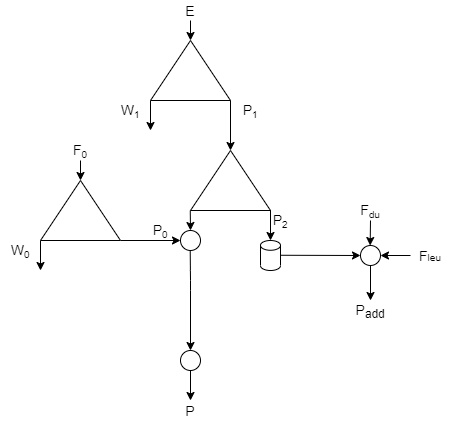
\includegraphics[scale=0.7]{cascades/P2utilization}}
  \caption{Схема независимого вовлечения загрязненногой изотопом $^{232}$U фракции с разбавлением обедненным и природным ураном}\label{P2utilization}
\end{figure}

\begin{table}[h]
  \centering
  \normalsize\begin{tabulary}{1.0\textwidth}{CCCCC}
  $^{232}$U & Цикл № & $P_2$, кг & Дополнительный продукт из $P_2$, доля новой ТВС, \% & Экономия природного урана, \% \\
  1.e-6\% & 2 & 1.09 & 7.11 & 14.6 \\
   & 5 & 0.92 & 10.21 & 6.3 \\
  5.e-7\% & 2 & 1.33 & 14.22 & 7.3 \\
   & 5 & 0.92 & 20.42 & 3.1 \\
  \end{tabulary}
  \caption{{Результаты вовлечения $P_2$ в производство дополнительного НОУ-продукта{\label{independent}}%
  }}
\end{table}

Принимая во внимание, что в конечном продукте двойного каскада НОУ-продукт требуемого качества был произведен в количестве, необходимом для одной ТВС (469 кг), масса $P_2$ и вклад этого побочного продукта в производство дополнительной ТВС приведены в табл. \ref{independent}. Так, значения в столбце <<Дополнительный продукт из $P_2$, доля новой ТВС \%>> соответствуют доле дополнительно произведенного НОУ из побочного $P_2$, образовавшегося в процессе обогащения топлива из регенерата для одной ТВС (469 кг).
Как мы могли видеть, предлагаемый способ использования $P_2$ позволяет экономить большее количество природного урана, чем двойной модифицированный каскад, в котором не предполагается задействование этого материала. Такой эффект более значителен для случаев, когда приходится иметь дело с побочным продуктом двойного каскада, образующимся на начальных циклах повторного использования (второй цикл в табл. \ref{independent}). Такая схема также показывает себя как более предпочтительная в экономии природного урана (вдвое выигрышнее, согласно табл. \ref{independent}), когда ПДК $^{232}$U получаемого таким способом продукта задается на уровне в два раза выше ($1\cdot10^{-7}$\% вместо $5\cdot10^{-7}$\%). Важно также показать следующие соотношения. Тогда как накопленный побочный продукт $P_2$ можно было бы использовать для производства дополнительных $\approx$7\% свежего НОУ-продукта для новой топливной сборки, это соответсвует возможности произвести дополнительную 15-ю сборку из накопленного $P_2$, образовавшегося при производстве предыдущих четырнадцати ТВС. Таким образом, для современного легководного реактора, такого как, например, российский ВВЭР-1200 или европейский PWR, где активная зона состоит из более чем 150 тепловыделяющих сборок, было бы изготовить дополнительно более 10 ТВС, взяв за основу предложенный способ. Значение экономии природного урана здесь соответствует доле $P_2$, смешанной с обедненным ураном $F_{du}$, до того, как он будет смешан с НОУ-разбавителем $F_{leu}$, полученным из природного урана. Эта пропорция также соответствует экономии на работы разделения, которая была бы затрачена в случае использования прямого обогащения природного урана в ординарном каскада без привлечения $P_2$.

Следует отметить, что рассмотренная схема имеет преимущество перед тройным каскадом (рис. \ref{fig:Tomsk}), заключающееся в том, что радиоактивными изотопами $^{232}$U и $^{234}$U будет загрязнена меньшая доля разделительного оборудования, поскольку в случае независимого вовлечения $P_2$, предложенного в диссертации, им не загрязняется дополнительные сепарационные мощности (газовые центрифуги).

\clearpage           % Глава 3
%\chapter*{Заключение}                       % Заголовок
\addcontentsline{toc}{chapter}{Заключение}  % Добавляем его в оглавление

%% Согласно ГОСТ Р 7.0.11-2011:
%% 5.3.3 В заключении диссертации излагают итоги выполненного исследования, рекомендации, перспективы дальнейшей разработки темы.
%% 9.2.3 В заключении автореферата диссертации излагают итоги данного исследования, рекомендации и перспективы дальнейшей разработки темы.
%% Поэтому имеет смысл сделать эту часть общей и загрузить из одного файла в автореферат и в диссертацию:

Основные результаты работы заключаются в следующем.
Теоретически обоснованы способы обогащения регенерированного урана с одновременной коррекцией его изотопного состава по содержанию четных изотопов, основанных на модификациях двойных каскадов. Показана применимость предложенных модификаций двойного каскада в условиях обогащения регенерированного урана с исходным содержанием четных изотопов выше допустимых пределов, что в несколько раз превышает содержание указанных изотопов в составах регенерата ранее рассмотренных в теоретических исследованиях. Это означает возможность успешного использования предложенных подходов в условиях многократного рецикла, когда концентрации четных изотопов возрастают от рецикла к рециклу.

По результатам проведенного исследования можно сформулировать следующие конкретные выводы.

\begin{enumerate}
\item В работе предложена модификация двойного каскада с НОУ-разбавителем из природного урана, применимая для обогащения регенерированного урана в условиях многократного рецикла урана в топливе легководных реакторов и позволяющая получить продукт, отвечающий всем требованиям на концентрации четных изотопов для регенерата различного исходного состава. Достоинствами схемы является возможность частичного отделения легких изотопов $^{232}$U, $^{234}$U от $^{235}$U, а также обособленность участков обогащения регенерированного урана и природного урана. Последнее обеспечивает большую вариативность в возможностях практической реализации подобной схемы, а также позволяет избежать загрязнения значительной части разделительного оборудования четными изотопами урана.


Процесс обогащения регенерата урана различного исходного состава в предложенной схеме смоделирован с использованием теории квазиидеального каскада. Разработаны оригинальные методики расчета и оптимизации предложенной каскадной схемы по различным критериям эффективности, таким как минимум расхода природного урана, минимум затрат работы разделения на получение конечного продукта, максимум степени извлечения целевого изотопа $^{235}$U из исходного регенерата и др. Проведена серия вычислительных экспериментов, позволившая оценить ключевые интегральные характеристики предложенной модификации двойного каскада (удельный расход природного урана, затраты работы разделения) в широком диапазоне изменение как ее параметров, так и внешних условий. Анализ результатов проведенных вычислительных экспериментов показал, что схема оказывается устойчивой в случаях, когда внешние ограничения <<ужесточаются>>. Например, уменьшается предельно допустимая концентрация $^{232}$U в товарном НОУ или кратно (до трех раз) возрастает масса исходного регенерированного урана, которую нужно израсходовать для получения заданной массы товарного продукта. Анализ полученных результатов создает базис для дальнейшей практической реализации подобной схемы и поиска наиболее эффективных режимов ее работы.

Анализ эффективности предложенной каскадной схемы с точки зрения потерь $^{235}$U показал, что схема позволяет извлечь более 85\% от массы $^{235}$U из исходного регенерированного урана, поступившего на обогащение. Это обеспечивает экономию природного урана по сравнению с открытым топливным циклом на уровне 15-20\% в зависимости от исходного изотопного состава регенерата. Таким образом, эта схема превышает аналогичные показатели для простейших разбавляющих схем практически вдвое.
\item Обоснован способ эффективной «утилизации» загрязненной четными изотопами фракции, возникающей в двойных каскадах при очистке от $^{232}$U, с учетом полной или частичной подачи данной фракции: а) в третий каскад с предварительным перемешиванием ее с природным, обедненным и/или низкообогащенным ураном; б) в отдельный двойной каскад, осуществляющий наработку низкообогащенного урана для последующей топливной кампании реактора. Для каждого из предложенных способов проведены вычислительные эксперименты, анализ результатов которых позволил сформулировать достоинства и недостатки каждого из способов и очертить возможные области их применения.
В качестве основных выводов по этой части приведем следующие:
\begin{enumerate}
\item Характерными недостатками схемы двойного каскада с НОУ-разбавителем с возвратом потока загрязненной $^{232}$U фракции в цикл является возврат значительной части четных изотопов на вход каскадной схемы. Это приводит к тому, что при повторении такого процесса несколько раз концентрации четных изотопов в исходном регенерате могут существенно возрастать (до нескольких раз), тем самым снижая эффективность обогащения регенерата в целом. Следовательно, такой подход применим для 1-3 таких возвратов, далее целесообразно рассмотреть возможность реализации одного из других предложенных способов утилизации отхода.
\item Характерным недостатком схемы тройного каскада для утилизации загрязненной $^{232}$U фракции является увеличение затрат работы разделения по отношению к другим рассмотренным модификациям, возникающее при обогащении разбавленного обедненным ураном загрязненного четными изотопами отхода. Анализ результатов серии вычислительных экспериментов, проведенных для данной схемы позволяет говорить, что она хорошо применима для составов регенерированного урана, когда исходное содержание $^{232}$U еще не превысило предельно допустимых значений для продукта. Иными словами, такой подход может подойти для обогащения регенерата 1-го и 2-го рецикла, позволяя вернуть в цикл более 90\% массы $^{235}$U из регенерированного урана. 
\item Схема утилизации загрязненной $^{232}$U фракции через ее разбавление обедненным ураном и НОУ из природного урана обеспечивает возможность наработки дополнительной массы отвечающего всем требованиям товарного продукта. При этом в схеме отсутствуют дополнительные каскады, что исключает дополнительные затраты работы разделения. Показано, что данный способ утилизации пригоден при обогащении различных вариантов составов исходного регенерата, что делает его перспективным в условиях многократного рецикла.
\end{enumerate}

\item Результаты работы дают основу для проведения дальнейшего технико-экономического анализа каждой из схем на основе их интегральных показателей, таких как расход природного урана, затраты работы разделения, потери $^{235}$U в цикле в контексте всей цепочки ядерного топливного цикла, а также с учетом возникающих в этой цепочке изменений при использовании регенерата урана по отношению к открытому топливному циклу. Помимо этого, необходима проработка технологических проблем каждой из схем, в частности, с точки зрения возможности эксплуатации и обслуживания оборудования в условиях работы с материалами, имеющими более высокую, чем природный уран удельную активность. 
\end{enumerate}



% В заключение автор выражает благодарность и большую признательность научному руководителю 
% Сулаберидзе~Г.\:А. и научному консультанту Смирнову А.Ю. за поддержку, помощь, обсуждение результатов и~научное
% руководство.



% Также автор благодарит Сидорова~А.\:А. и~Петрова~Б.\:Б.
% за помощь в~работе с~образцами, Рабиновича~В.\:В. за предоставленные
% образцы и~обсуждение результатов, Занудятину~Г.\:Г. и авторов шаблона
% *Russian-Phd-LaTeX-Dissertation-Template* за~помощь в оформлении
% диссертации. Автор также благодарит много разных людей
% и~всех, кто сделал настоящую работу автора возможной.
      % Заключение
\chapter*{Список сокращений и условных обозначений} % Заголовок
\addcontentsline{toc}{chapter}{Список сокращений и условных обозначений}  % Добавляем его в оглавление
\noindent
%\begin{longtabu} to \dimexpr \textwidth-5\tabcolsep {r X}
\begin{longtabu} to \textwidth {r X}
% Жирное начертание для математических символов может иметь
% дополнительный смысл, поэтому они приводятся как в тексте
% диссертации

\(q_0\) & коэффициент разделения\\
\(N\) & длина каскада (число ступеней)\\

\(\begin{rcases}
f\\
N+1-f
\end{rcases}\)  &
число ступеней в обеднительной и обогатительной частях.
\\

\(\begin{rcases}
    n\\
    k
    \end{rcases}\)  &
    индексы целевого ($^{235}$U) и опорного компонент.
\\

\(\begin{rcases}
    F_i\\
    P_i\\
    W_i
    \end{rcases}\)  &
    потоки питания, отбора и отвала, где \textit{i} -- индекс каскада.
\\



\textbf{ЛВР} & легководный реактор \\
\textbf{ВВЭР} & водо-водяной энергетический реактор \\
\textbf{ЯТЦ} & ядерный топливный цикл \\
\textbf{ЗЯТЦ} & замкнутый ядерный топливный цикл \\
\textbf{ТВС} & тепловыделяющая сборка \\
\textbf{MOX-топливо} & ядерное топливо, состоящее из смеси диоксидов урана и плутония \\
\textbf{ОЯТ} & Облученное ядерное топливо, извлеченное из ядерного реактора после использования и для этой цели в имеющейся форме более непригодноe \\

\textbf{РАО} & Радиоактивные отходы. Существуют подклассы радиоактивных отходов: высокоактивные (ВАО), среднеактивные (САО), низкоактивные (НАО) \\




\textbf{НОУ} & низкообогащенный уран \\
\textbf{ВОУ} & высокообогащенный уран\\
%\textbf{RepU} & регенерированный уран \\
\textbf{ОГФУ} & обедненный гексафторид урана\\

\textbf{РР} & работа разделения\\
\textbf{ЕРР} & 1 кг работы разделения, единица работы по разделению изотопов. Мера усилий, затрачиваемых на разделение материала определённого изотопного состава на две фракции с отличными изотопными составами; не зависит от применяемого процесса разделения. \\

\textbf{$UF_6$} & гексафторид урана\\
\textbf{$C_{8}H_{3}F_{13}$} & фреон-346\\

\textbf{ASTM} & международное общество по испытаниям и материалам\\
\textbf{ASTM} & международное общество по испытаниям и материалам\\


\textbf{СНАУ} & система нелинейных алгебраических уравнений \\

%\textbf{Toxic Waste} & смесь с высоким содержанием минорных изотопов, классифицируемая как токсичный отход, требующий дорогостоящего хранения\\
%\textbf{mix} & смешение изотопных композиций\\


\end{longtabu}

Критерии эффективности каскадной схемы:
\begin{itemize}
    \item $(Y_f)_\text{max}$ -- максимум суммарной степени извлечения схемы (\ref{Rec2}) , соответствующий минимуму потерь $^{235}$U в схеме;
    \item $(Y_{RepU})_\text{max}$ -- максимум степени извлечения из регенерата (\ref{RecR2}), соответствующий минимуму потерь $^{235}$U регенерата;
    \item $(\delta(\frac{\Delta A}{P}))_\text{min}$ -- максимум экономии работы разделения, относительно референтной схемы трехпоточного каскада для обогащения природного урана, соответствующая минимуму удельного расхода работы разделения; 
    \item $(\delta(\frac{F_{NU}}{P}))_\text{min}$\ -- максимальная экономия природного урана относительно референтной схемы трехпоточного каскада для обогащения природного урана, соответствующая минимуму удельного расхода природного урана.
\end{itemize}\label{criteria_list}

Обозначения параметров каскадных схем:
\begin{itemize}
    \item $Y_f$ -- суммарная степень извлечения $^{235}$U в схеме \ref{Rec2};
    \item $Y_{RepU}$ -- степень извлечения $^{235}$U схемой из регенерированного урана \ref{RecR2};
    \item $\delta(\frac{\Delta A}{P})$ -- экономия работы разделения относительно референтной схемы трехпоточного каскада для обогащения природного урана. Наибольшая экономия соответствует минимуму суммарного потока схемы \ref{GrindEQ__1_73_}. Если величина отрицательная, абсолютное значение соответствует потерям работы разделения, по сравнению с референтной схемы трехпоточного каскада для обогащения природного урана.
    \item  $\frac{F_{NU}}{P}$ -- удельный расход природного урана на единицу производимого товарного НОУ;
    \item  $\delta(\frac{F_{NU}}{P})$ -- экономия природного урана относительно референтной схемы трехпоточного каскада для обогащения природного урана.  Наибольшая экономия соответствует минимуму удельного расхода природного урана схемы. Если величина отрицательная, абсолютное значение соответствует перерасходу природного урана, по сравнению с референтной схемы трехпоточного каскада для обогащения природного урана;
    \item $M_{k1}$ -- масса изотопа, выбранного в качестве опорного компонента при расчете R-каскада (\ref{GrindEQ__1_75_})--(\ref{GrindEQ__1_76_}), для первого каскада в схеме, в который поступает регенерат;
    \item $M_{k2}$ -- масса изотопа, выбранного в качестве опорного компонента при расчете R-каскада (\ref{GrindEQ__1_75_})--(\ref{GrindEQ__1_76_}), для второго каскада в схеме, на питание которого поступает поток легкой фракции первого каскада;
    \item $C_{232,\text{P}},C_{234,\text{P}},C_{235,\text{P}},C_{236,\text{P}}$ -- концентрации изотопов урана в конечном НОУ-продукте $P$;
    \item $C_{232,\text{x}},C_{234,\text{x}},C_{235,\text{x}},C_{236,\text{x}}$ -- концентрации изотопов урана в потоках $x$;
    \item $F_{x}$ -- выходные потоки, выраженные в килограммах гексафторида урана ($UF_6$), получаемые в схеме при производстве 1 тонны металического урана НОУ-продукта.
  \end{itemize}
  
\addtocounter{table}{-1}% Нужно откатить на единицу счетчик номеров таблиц, так как предыдущая таблица сделана для удобства представления информации по ГОСТ
        % Список сокращений и условных обозначений
%\chapter*{Словарь терминов}             % Заголовок
\addcontentsline{toc}{chapter}{Словарь терминов}  % Добавляем его в оглавление

\textbf{TeX} : Cистема компьютерной вёрстки, разработанная американским профессором информатики Дональдом Кнутом

\textbf{панграмма} : Короткий текст, использующий все или почти все буквы алфавита
      % Словарь терминов
\clearpage                                  % В том числе гарантирует, что список литературы в оглавлении будет с правильным номером страницы
%\hypersetup{ urlcolor=black }               % Ссылки делаем чёрными
%\providecommand*{\BibDash}{}                % В стилях ugost2008 отключаем использование тире как разделителя
\urlstyle{rm}                               % ссылки URL обычным шрифтом
\ifdefmacro{\microtypesetup}{\microtypesetup{protrusion=false}}{} % не рекомендуется применять пакет микротипографики к автоматически генерируемому списку литературы
\insertbibliofull                           % Подключаем Bib-базы: все статьи единым списком
% Режим с подсписками
%\insertbiblioexternal                      % Подключаем Bib-базы: статьи, не являющиеся статьями автора по теме диссертации
% Для вывода выберите и расскомментируйте одно из двух
%\insertbiblioauthor                        % Подключаем Bib-базы: работы автора единым списком 
%\insertbiblioauthorgrouped                 % Подключаем Bib-базы: работы автора сгруппированные (ВАК, WoS, Scopus и т.д.)
\ifdefmacro{\microtypesetup}{\microtypesetup{protrusion=true}}{}
\urlstyle{tt}                               % возвращаем установки шрифта ссылок URL
%\hypersetup{ urlcolor={urlcolor} }          % Восстанавливаем цвет ссылок      % Список литературы

%%% Настройки для приложений
\appendix
% Оформление заголовков приложений ближе к ГОСТ:
\setlength{\midchapskip}{20pt}
\renewcommand*{\afterchapternum}{\par\nobreak\vskip \midchapskip}
\renewcommand\thechapter{\Asbuk{chapter}} % Чтобы приложения русскими буквами нумеровались

\chapter{}\label{app:A}

\section{Список публикаций}\label{app:A1}

\begin{enumerate}
	\item Scopus:
    \begin{enumerate}
        \item A.Yu. Smirnov, G.A. Sulaberidze, V. E. Gusev, Е.А. Andrianova, V. Yu. Blandinski, А.V. Grol, A.A. Dudnikov, V.A. Nevinitsa, P.A. Fomichenko. Applying enrichment capacities for multiple recycling of LWR uranium //  J. Phys.: Conf. Ser. 2018. V. 1099. 012001 (doi :10.1088/1742-6596/1099/1/012001)
        \item Smirnov A., Gusev V., Sulaberidze G., Nevinitsa V. A method to enrich reprocessed uranium with various initial contents of even-numbered isotopes // AIP Conference Proceedings Volume 2101, Номер статьи 020006.
        \item Gusev V.E., Smirnov A.Y., Volkov Y.N., Sulaberidze G.A., Blandinski V.Y., Grol A.V., Nevinitsa V.A. Features of light-water reactor fuel made of reprocessed uranium in terms of IAEA safeguards implementation // Journal of Physics: Conference Series
        Volume 1133, Issue 1, 2018, Номер статьи 012041
        \item Gusev V.E., Smirnov A.Yu., Sulaberidze G.A., Nevinitsa V.A. The role of Gas Centrifuge Cascades in Uranium Recycling // KERNTECHNIK (Отправлена в журнал в 2019 году (первая половина), находится на рецензировании).
    \end{enumerate}
    \item ВАК:
    \begin{enumerate}
        \item Смирнов А.Ю., Гусев В.Е., Сулаберидзе Г.А., Невиница В.А., Фомиченко П.А. ОБОГАЩЕНИЕ РЕГЕНЕРИРОВАННОГО УРАНА В ДВОЙНОМ КАСКАДЕ ГАЗОВЫХ ЦЕНТРИФУГ С ЕГО МАКСИМАЛЬНЫМ ВОЗВРАТОМ В ВОСПРОИЗВОДСТВО ТОПЛИВА // Вестник НИЯУ МИФИ. 2018. Т.7. № 6. С. 449-457
        \item В. А. Невиница, А. Ю. Смирнов, Г. А. Сулаберидзе, В. Е. Гусев, А. М. Павловичев, А. И. Щеренко, Е. В. Родионова, В. Ю. Бландинский. Топливный цикл легководного реактора с полным использованием регенерированного урана // Вестник НИЯУ МИФИ (Отправлена в редакцию 19.09.2019)
        \item Е. В. Родионова, А. Ю. Смирнов, В. А. Невиница, Г. А. Сулаберидзе, В. Е. Гусев, В. Ю. Бландинский, С. В. Цибульский. Анализ технико-экономических характеристик двойной каскадной схемы для обогащения многократно рециклированного регенерированного урана // Вопросы атомной науки и техники, сер. Физика ядерных реакторов. (Отправлена в редакцию, принята к печати)
        \item В. А. Невиница, А. Ю. Смирнов, Г. А. Сулаберидзе, В. Е. Гусев,
        А. М. Павловичев, А. И. Щеренко, Е. В. Родионова, В. Ю. Бландинский. ТОПЛИВНЫЙ ЦИКЛ ЛЕГКОВОДНОГО РЕАКТОРА С ПОЛНЫМ ИСПОЛЬЗОВАНИЕМ РЕГЕНЕРИРОВАННОГО УРАНА, ВЕСТНИК НАЦИОНАЛЬНОГО ИССЛЕДОВАТЕЛЬСКОГО ЯДЕРНОГО УНИВЕРСИТЕТА “МИФИ”, 2019, том 8, № 6,
        с. 498–506.
        \item Смирнов А.Ю., Гусев В.Е., Сулаберидзе Г.А., Невиница В.А., Фомиченко П.А. Анализ влияния ограничений по изотопам 232,234,236U в товарном НОУ на выбор способов обогащения регенерата урана в каскадах центрифуг //  Вопросы атомной науки и техники, сер. Физика ядерных реакторов. (Отправлена в редакцию в декабре 2018 года, принята к печати).
        \end{enumerate}
\end{enumerate}

\section{Участие в конференциях}~\label{app:A2}

\begin{enumerate}
    \item В качестве доклачика:
    \begin{enumerate}
        \item Конференция:  XVII International conference and School for young scholars “Physical chemical processes in atomic systems”, г. Москва, Россия. Доклад: ENRICHMENT SCHEMES FOR REPROCESSED URANIUM RECYCLING, Авторы: V.E. Gusev.
    \end{enumerate}
    \item В качестве соавтора:
    \begin{enumerate}
        \item Конференция:  15th International Workshop on Separation Phenomena in Liquids and Gases (SPLG-2019), г. Уси, Китай. Доклад: Method of Reprocessed Uranium Enrichment for NPP Fuel Supply, Авторы: A. Yu. Smirnov, V.E. Gusev, G.A.Sulaberidze
        \item Конференция:  XVII International conference and School for young scholars “Physical chemical processes in atomic systems”, г. Москва, Россия. Доклад: Physical regularities of recycling of recovered nuclear materials (uranium         and plutonium) in thermal reactor fuel, Авторы: A. Yu. Smirnov, G.A.Sulaberidze, V.E. Gusev, V.A. Nevinitsa
    \end{enumerate}
\end{enumerate}

Стажировки:
    \begin{enumerate}
        \item IV International Summer School on Engineering Computing in Nuclear Technology ECINT School 2019 (с сертификатом)
    \end{enumerate}
        % Приложения

\end{document}
